\providecommand{\toplevelprefix}{../..}
\documentclass[../../book-main_ro.tex]{subfiles}

\begin{document}

\chapter{Învățarea Reprezentărilor pentru Date din Lumea Reală}
\label{ch:applications}

\begin{quote}
\hfill    ``{\em Cea mai bună teorie este inspirată de practică, iar cea mai bună practică este inspirată de teorie}.''

$~$ \hfill --- Donald Knuth   
\end{quote}
\vspace{5mm}

Capitolele anterioare au prezentat o introducere sistematică în problemele matematice, cadrele computaționale și algoritmii practici asociați cu învățarea distribuțiilor de dimensiune redusă din date de dimensiune înaltă. Deși majoritatea justificărilor teoretice ale acestor metode au fost stabilite pentru modele idealiste de date, cum ar fi (amestecuri de) subspații și/sau Gaussiane, principiile și ideile din spatele acestor metode computaționale sunt totuși puternice și generale, și sunt de fapt menite să fie aplicabile pentru seturi de date și sarcini din lumea reală.

Pentru a ajuta cititorii să înțeleagă mai bine materialul din această carte și să învețe cum să aplice ceea ce ați învățat până acum la date din lumea reală, spre sfârșitul cărții, oferim câteva demonstrații și viniete ale mai multor aplicații reprezentative. Fiecare aplicație propune o soluție la o sarcină din lumea reală cu un set de date din lumea reală (cum ar fi date vizuale și date text), folosind metodele pe care le-am introdus în această carte. Rezultatele prezentate în acest capitol sunt menite să servească următoarele două scopuri:
\begin{itemize}
    \item în primul rând, să ofere detalii experimentale suplimentare și dovezi empirice care validează metodele prezentate mai devreme în carte și demonstrează potențialul lor semnificativ în contexte din lumea reală;
    \item în al doilea rând, să introducă cititorul în anumite metode și sarcini empirice moderne în învățarea profundă care nu sunt bine documentate în afara bazelor de cod de cercetare sau producție.
\end{itemize}
Cu toate acestea, în opinia noastră sinceră, soluțiile și rezultatele date aici sunt concepute pur și simplu pentru a verifica că metodologia funcționează. Ca atare, există mult spațiu pentru îmbunătățiri viitoare, atât în inginerie cât și în înțelegerea teoretică, pentru a îmbunătăți potențial starea actuală a artei. Vom discuta câteva direcții viitoare în \Cref{ch:future}.




\section{Configurare Tehnică și Schema Capitolului}\label{sec:experiment_setup}

În capitolele anterioare, am făcut aluzie la diferite configurări în care am folosit tehnici de învățare a reprezentărilor pentru a procesa date reale la scară. În acest capitol, vom descrie astfel de configurări în detaliu mare. Obiectivul acestei secțiuni este să vă facem pe dumneavoastră, cititorul, să puteți reproduce orice experiment discutat în această secțiune (sau într-adevăr în carte) folosind doar descrierea pe care o vom da în carte, principiile introduse în capitolele anterioare și extinse în acest capitol, și hiperparametri luați dintr-o serie de lucrări ale căror rezultate sunt discutate în acest capitol. În acest scop, vom descrie \textit{precis} toate procedurile într-un limbaj detaliat, pseudocod sau notație matematică care pot fi implementate direct în cod. Oriunde este posibil, vom discuta cum se conectează implementările concrete la principiile prezentate mai devreme în carte.

\begin{figure}
    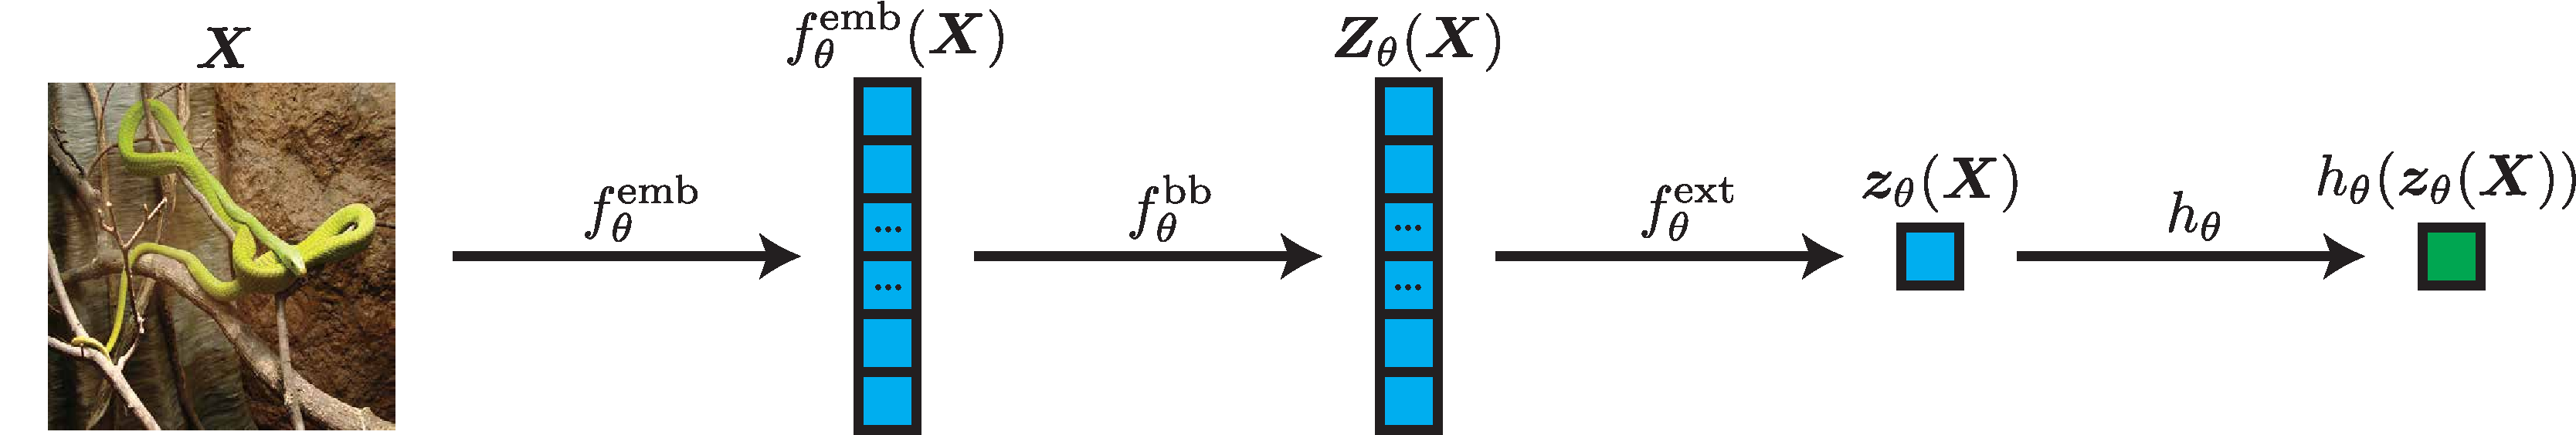
\includegraphics[width=\textwidth]{\toplevelprefix/chapters/chapter7/figs/encoder_pipeline.pdf}
    \caption{\small\textbf{O diagramă a pipeline-ului encoder.} Datele \(\vX \in \cD\) sunt introduse prin încorporarea \(f_{\theta}^{\emb}\) pentru a obține o secvență în \((\R^{d})^{*}\). Încorporarea este introdusă printr-o coloană vertebrală \(f_{\theta}^{\mathrm{bb}}\) pentru a obține caracteristici \(\vZ_{\theta}(\vX)\) pentru fiecare token. Putem extrage o caracteristică agregată \(\vz_{\theta}(\vX)\) folosind harta de extracție \(f_{\theta}^{\mathrm{ext}}\). În cele din urmă, pentru a folosi caracteristica agregată în sarcini în aval, putem folosi capul specific sarcinii \(h_{\theta}\).}
    \label{fig:overall_encoder_pipeline}
\end{figure}

\begin{figure}
    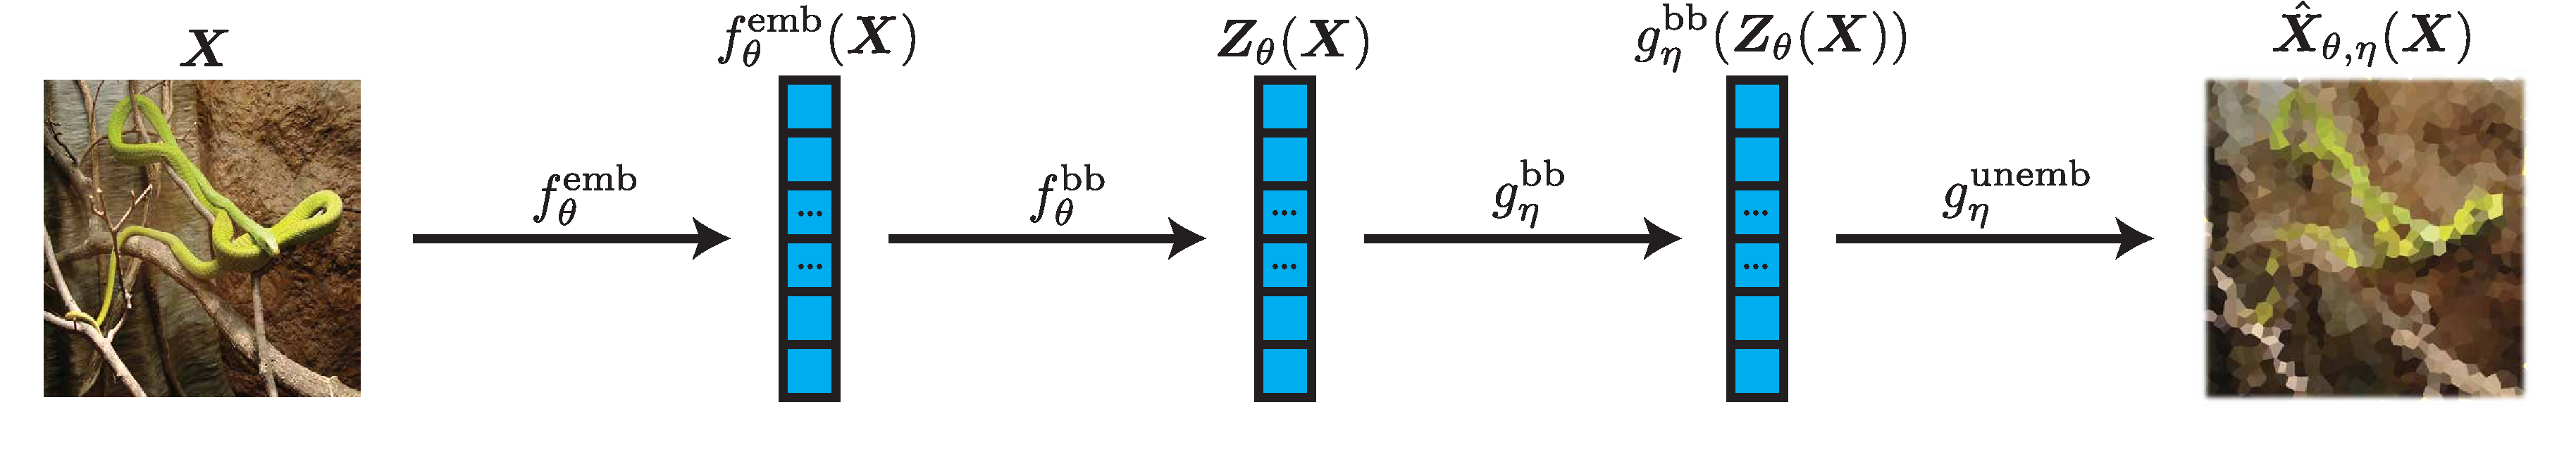
\includegraphics[width=\textwidth]{\toplevelprefix/chapters/chapter7/figs/autoencoder_pipeline.pdf}
    \caption{\small\textbf{O diagramă a pipeline-ului autoencoder.} Datele \(\vX \in \cD\) sunt introduse prin încorporarea \(f_{\theta}^{\emb}\) pentru a obține o secvență în \((\R^{d})^{*}\). Încorporarea este introdusă printr-o coloană vertebrală encoder \(f_{\theta}^{\mathrm{bb}}\) pentru a obține caracteristici \(\vZ_{\theta}(\vX)\) pentru fiecare token. Pentru a decoda \(\vZ_{\theta}(\vX)\), o trecem printr-o coloană vertebrală decoder \(g_{\eta}^{\mathrm{bb}}\). Pentru a mapa ieșirea coloanei vertebrale decoder înapoi în spațiul datelor \(\cD\), folosim un strat de \textit{dezîncorporare} \(g_{\eta}^{\mathrm{unemb}}\), obținând în general o reconstrucție \(\hat{\vX}_{\theta, \eta}(\vX)\) (aici stilizată să fie o reconstrucție pixelată a intrării).}
    \label{fig:overall_autoencoder_pipeline}
\end{figure}

Să definim setul de date posibile ca \(\cD\) (în cele din urmă acesta va fi setul de imagini \(\cI\), de exemplu, sau setul de text \(\cT\)), și setul de secvențe finite de token-uri în \(\R^{d}\) (adică, setul de matrice cu \(d\) rânduri) ca \((\R^{d})^{*} \doteq \bigcup_{T = 1}^{\infty}\R^{d \times T}\). Pentru a discuta bogăția de aplicații pe care le introducem în acest capitol, ne amintim mai întâi că în restul cărții, discutăm două tipuri diferite de arhitecturi de model.
\begin{itemize}
    \item O arhitectură \textit{encoder}, parametrizată de \(\theta\), care este compusă din mai multe componente:
    \begin{itemize}
        \item O \textit{încorporare} \(f_{\theta}^{\emb} \colon \cD \to (\R^{d})^{*}\), care convertește datele de intrare \(\cD\) într-o serie de \textit{token-uri} care sunt mapate în, sau \textit{încorporate} în, spațiul \(d\)-dimensional. \textit{În restul capitolului, vom identifica adesea token-urile și încorporările unul cu celălalt.}
        \item O \textit{coloană vertebrală encoder} \(f_{\theta}^{\backbone} \colon (\R^{d})^{*} \to (\R^{d})^{*}\), care procesează seria de încorporări folosind o operație secvență-la-secvență. Această coloană vertebrală este implementată de arhitecturile de rețea discutate în capitolele anterioare, dar vom da o descriere mai formală pe măsură ce avansăm.
        \item Un \textit{extractor de caracteristici agregate} \(f_{\theta}^{\ext} \colon (\R^{d})^{*} \to \R^{d}\), care extrage o reprezentare agregată a întregii secvențe. Aceasta este folosită pentru a defini o singură caracteristică pentru întreaga mostră de date.
        \item Un \textit{cap specific sarcinii} \(h_{\theta} \colon \R^{d} \to \R^{m}\), care extrage o ieșire \(m\)-dimensională pentru predicție.
    \end{itemize}
    De asemenea, definim \(f_{\theta} \doteq f_{\theta}^{\backbone} \circ f_{\theta}^{\emb} \colon \cD \to (\R^{d})^{*}\). Dată o intrare \(\vX\), scriem \(\vZ_{\theta}(\vX) \doteq f_{\theta}(\vX)\) și \(\vz_{\theta}(\vX) \doteq f_{\theta}^{\ext}(\vZ_{\theta}(\vX))\). Pipeline-ul general este ilustrat în \Cref{fig:overall_encoder_pipeline}.
    \item O arhitectură \textit{autoencoder}, care este compusă din mai multe componente:
    \begin{itemize}
        \item O \textit{încorporare} \(f_{\theta}^{\emb} \colon \cD \to (\R^{d})^{*}\), care convertește datele de intrare \(\cD\) într-o serie de \textit{token-uri} care sunt încorporate în spațiul \(d\)-dimensional.
        \item O \textit{coloană vertebrală encoder} \(f_{\theta}^{\backbone} \colon (\R^{d})^{*} \to (\R^{d})^{*}\), care procesează seria de încorporări folosind o operație secvență-la-secvență.
        \item O \textit{coloană vertebrală decoder} \(g_{\eta}^{\backbone} \colon (\R^{d})^{*} \to (\R^{d})^{*}\), care anulează conceptual operația coloanei vertebrale encoder.
        \item O \textit{dezîncorporare} \(g_{\eta}^{\unemb} \colon (\R^{d})^{*} \to \cD\), care acționează ca o inversă a încorporării.
    \end{itemize}
    De asemenea, definim \(f_{\theta} \doteq f_{\theta}^{\backbone} \circ f_{\theta}^{\emb} \colon \cD \to (\R^{d})^{*}\) și \(g_{\eta} \doteq g_{\eta}^{\unemb} \circ g_{\eta}^{\backbone} \colon (\R^{d})^{*} \to \cD\). Dată o intrare \(\vX\), scriem \(\vZ_{\theta}(\vX) \doteq f_{\theta}(\vX)\) și \(\hat{\vX}_{\theta, \eta}(\vX) \doteq g_{\eta}(\vZ_{\theta}(\vX))\). Pipeline-ul general este ilustrat în \Cref{fig:overall_autoencoder_pipeline}.
\end{itemize}

Vom folosi în mod repetat această notație de multe ori în acest capitol, așa că vă rugăm să vă simțiți liberi să vă referiți înapoi la ea dacă ceva nu are sens. Această descompunere a rețelelor noastre oglindește de asemenea îndeaproape majoritatea implementărilor de cod, și puteți începe proiectele dvs. de codare prin definirea acestor rețele.

În acest capitol, vom discuta aplicațiile principiilor cărții la învățarea contrastivă în \Cref{sec:contrastive_learning}. Aceasta va servi atât ca o introducere în datele de imagine, tehnicile de augmentare a datelor și arhitectura comună cunoscută sub numele de transformer, \textit{precum și} o primă demonstrație a tipurilor drastice de simplificări pe care le putem face folosind principiile demonstrate. Vom continua cu modificări ale \textit{arhitecturii rețelei} în \Cref{sec:image_classification,sec:clm_text}, care demonstrează capacitățile arhitecturilor simplificate pentru \textit{encodare} în domeniile imagine și text. Apoi demonstrăm arhitecturi simplificate pentru \textit{autoencodare} în \Cref{sec:image_completion}.


\section{Învățare Contrastivă Simplificată}\label{sec:contrastive_learning}

Învățarea reprezentărilor de înaltă calitate și fidele ale datelor este o problemă fundamentală în învățarea profundă, cunoscută sub numele de \textit{învățare auto-supervizată}. Au fost propuse multe abordări pentru această sarcină, multe dintre ele nefolosind în mod evident tehnicile și principiile prezentate în acest manuscris. O astfel de abordare se numește \textit{învățare contrastivă}, numită astfel deoarece obiectivul de învățare este (vorbind în general) despre asigurarea că caracteristicile datelor „similare" sunt similare, iar caracteristicile datelor „disimilare" sunt departe. Soluțiile de învățare contrastivă sunt adesea abordări foarte inginerești, concepute empiric. În această secțiune, vom descrie o astfel de abordare numită DINO \citep{caron2021emerging} și vom folosi principiile descrise în capitolele anterioare pentru a simplifica drastic deciziile lor de design, îmbunătățind în același timp reprezentările învățate.

\subsection{Date}\label{sub:contrastive_learning_data}

Datele pe care le vom folosi pentru a explora și simplifica metodologia DINO sunt toate date de imagine bidimensionale. Pentru \textit{antrenament}, vom folosi seturile de date ImageNet-1K și ImageNet-21K. Fiecare mostră din setul de date este o imagine RGB, de rezoluție variabilă, și o etichetă care indică obiectul sau scena pe care o conține imaginea (adică, \textit{clasa} imaginii). Setul de date ImageNet-1K conține 1,28M imagini de antrenament și 50K imagini de validare partiționare în 1K clase. Setul de date ImageNet-21K conține 14,2M imagini de antrenament și 21,8K clase, dar clasele nu sunt disjuncte (adică, unele clase sunt subseturi ale altora). Deoarece facem învățare auto-supervizată, etichetele nu vor fi folosite în timpul antrenamentului, doar în timpul evaluării. Pentru \textit{evaluare}, vom folosi o multitudine de seturi de date. Dintre acestea, cel mai comun este CIFAR-10. CIFAR-10 este un set de date de 60K imagini naturale RGB 32 \(\times\) 32 partiționare în 10 clase, cu un set de antrenament prestabilit de 50K mostre și un set de validare de 10K mostre. Scopul utilizării CIFAR-10 este de a ne asigura că modelele care se antrenează pe o distribuție de imagini (ImageNet) pot generaliza la o altă distribuție de imagini (CIFAR-10). Ne referim de asemenea la alte seturi de date similare, cum ar fi CIFAR-100 (disjunct de CIFAR-10), Oxford Flowers și Oxford Pets. Exemplare de date ImageNet-1K și CIFAR-10 sunt prezentate în \Cref{fig:in1k_cifar10_examples}. Pentru a crește robustețea modelului nostru, aplicăm adesea \textit{augmentări mici de date} la fiecare imagine în timpul procesării, cum ar fi răsturnări, adăugarea de zgomot aleatoriu mic sau decupări aleatorii mari; nu includem acest lucru în notația noastră, deoarece fiecare augmentare a unei imagini naturale este ea însăși (foarte aproape de) o imagine naturală în setul nostru de date.

\begin{figure}
    \centering
    
    \hfill 
    \begin{subfigure}{0.3\textwidth}
        \centering 
        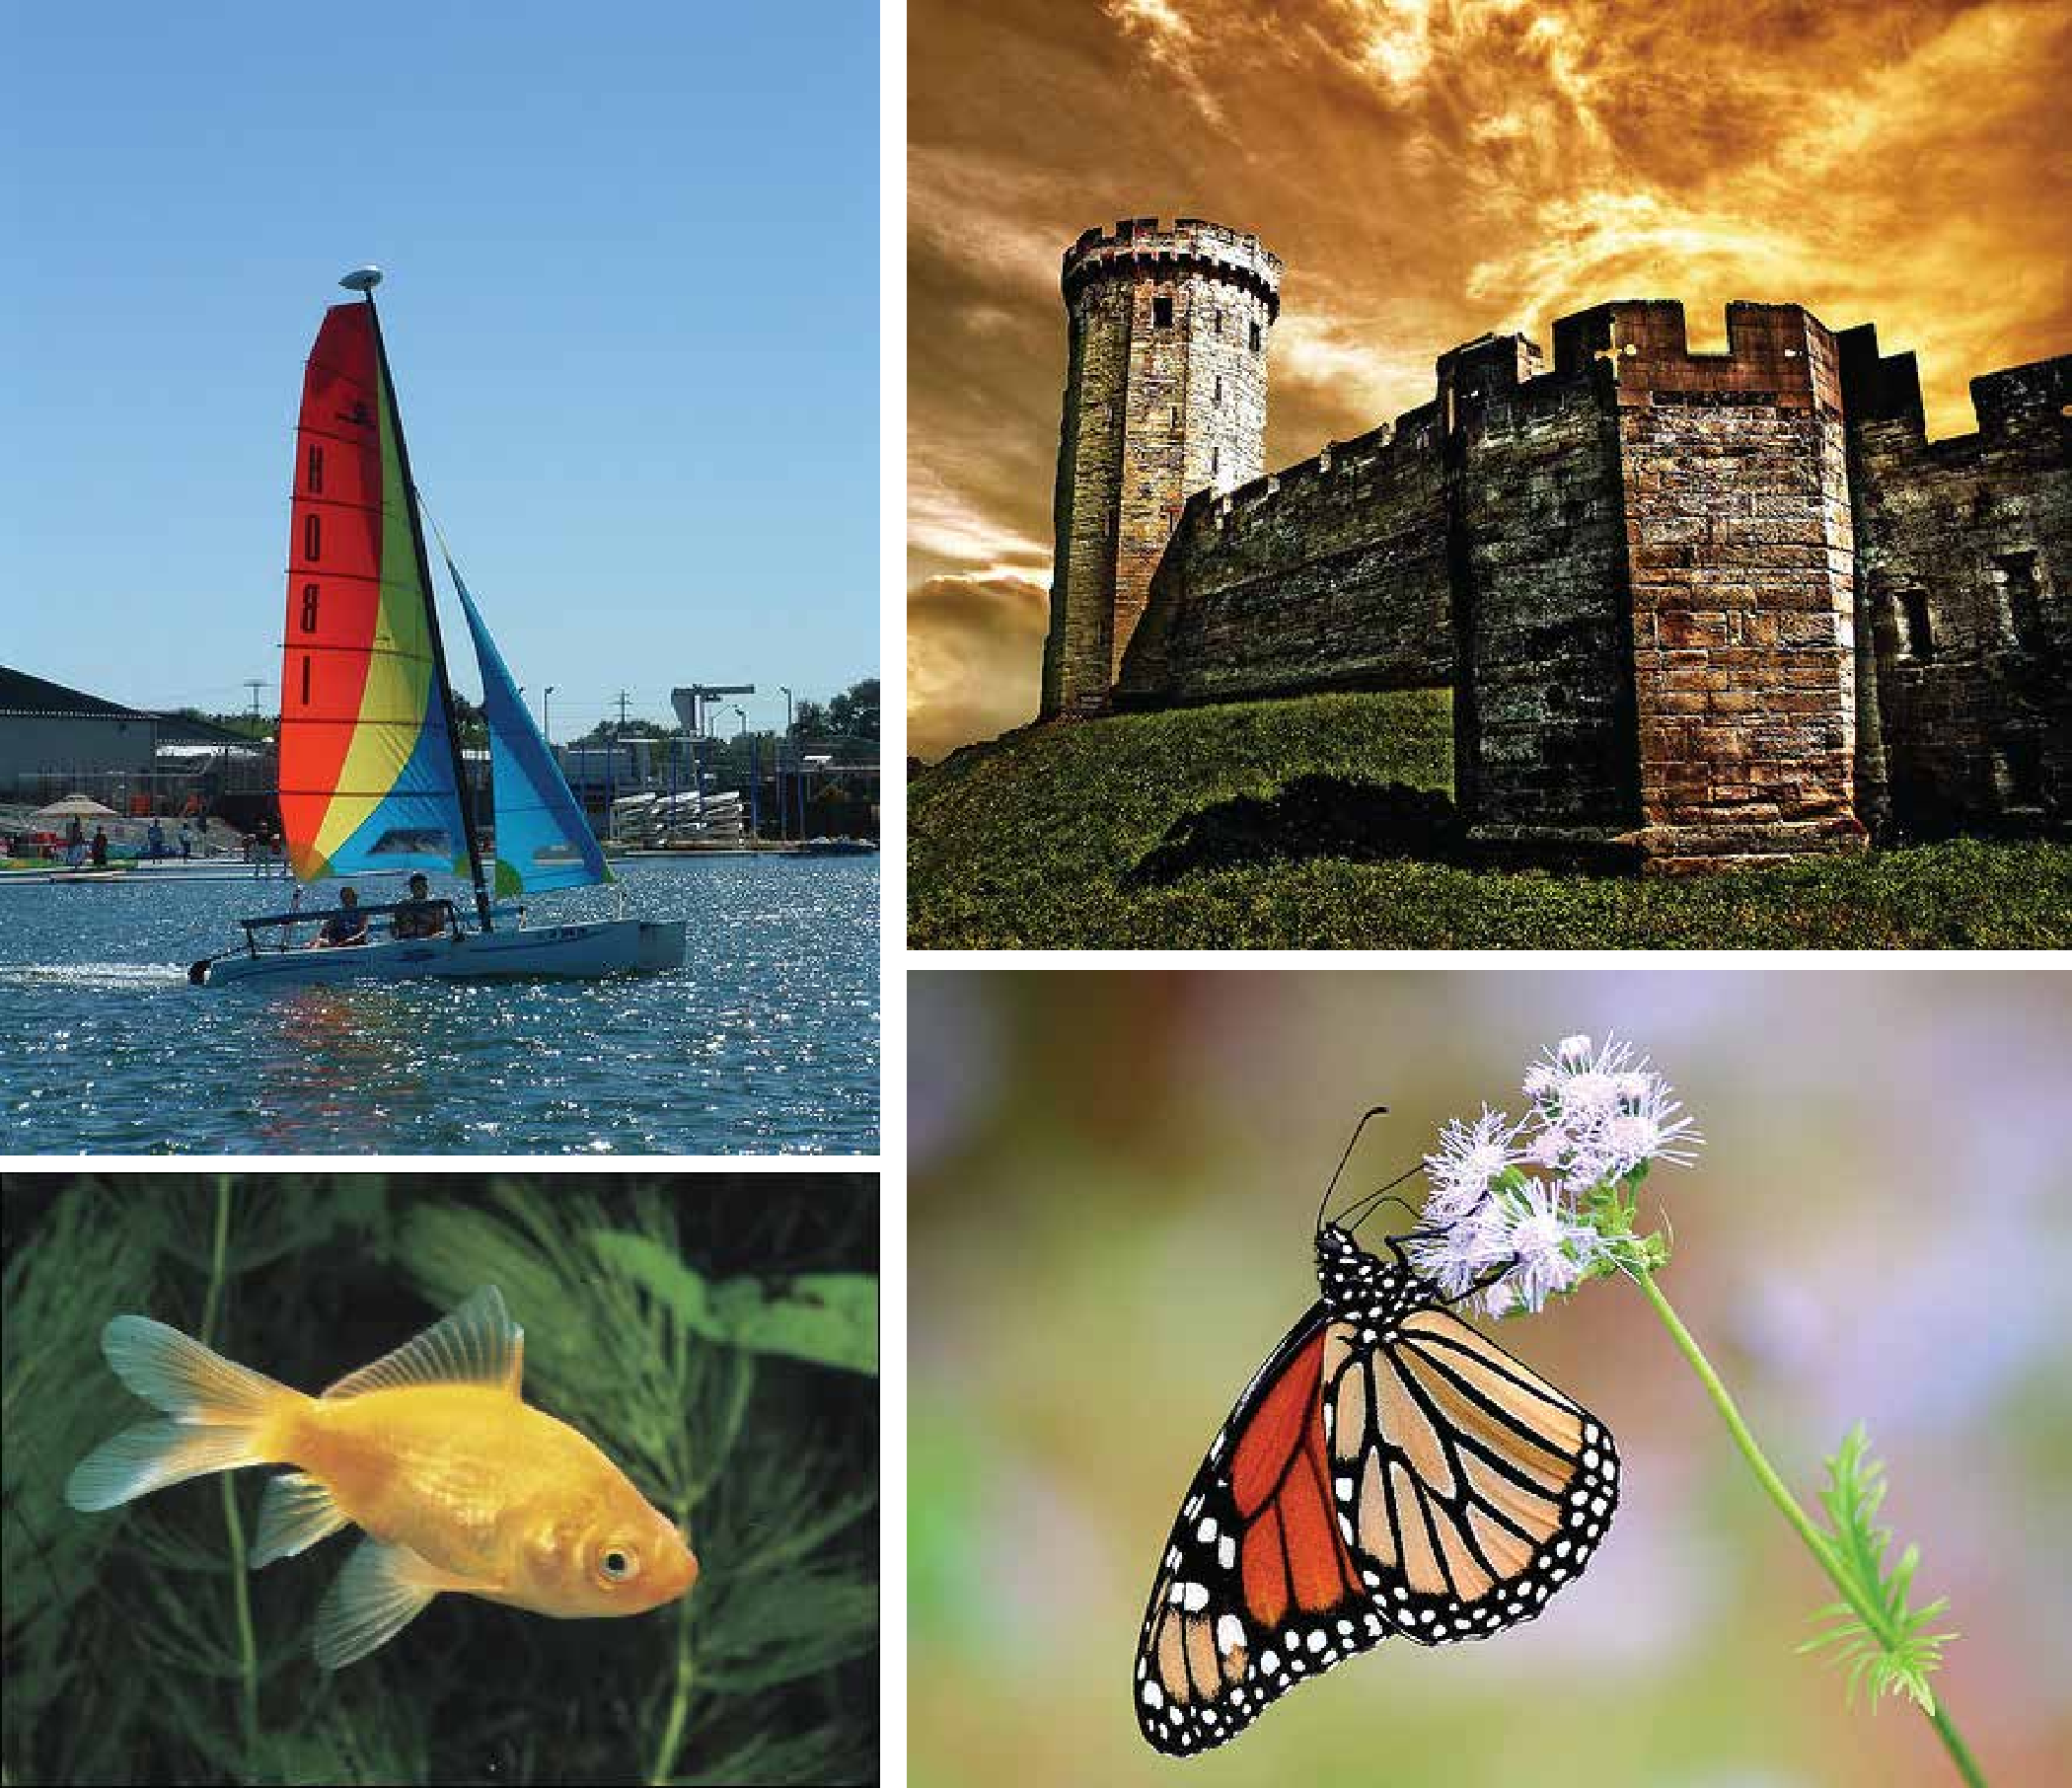
\includegraphics[width=\textwidth]{\toplevelprefix/chapters/chapter7/figs/imagenet.pdf}
        \caption{\small Mostre ImageNet-1K.}
    \end{subfigure}
    \hfill 
    \begin{subfigure}{0.26\textwidth}
        \centering 
        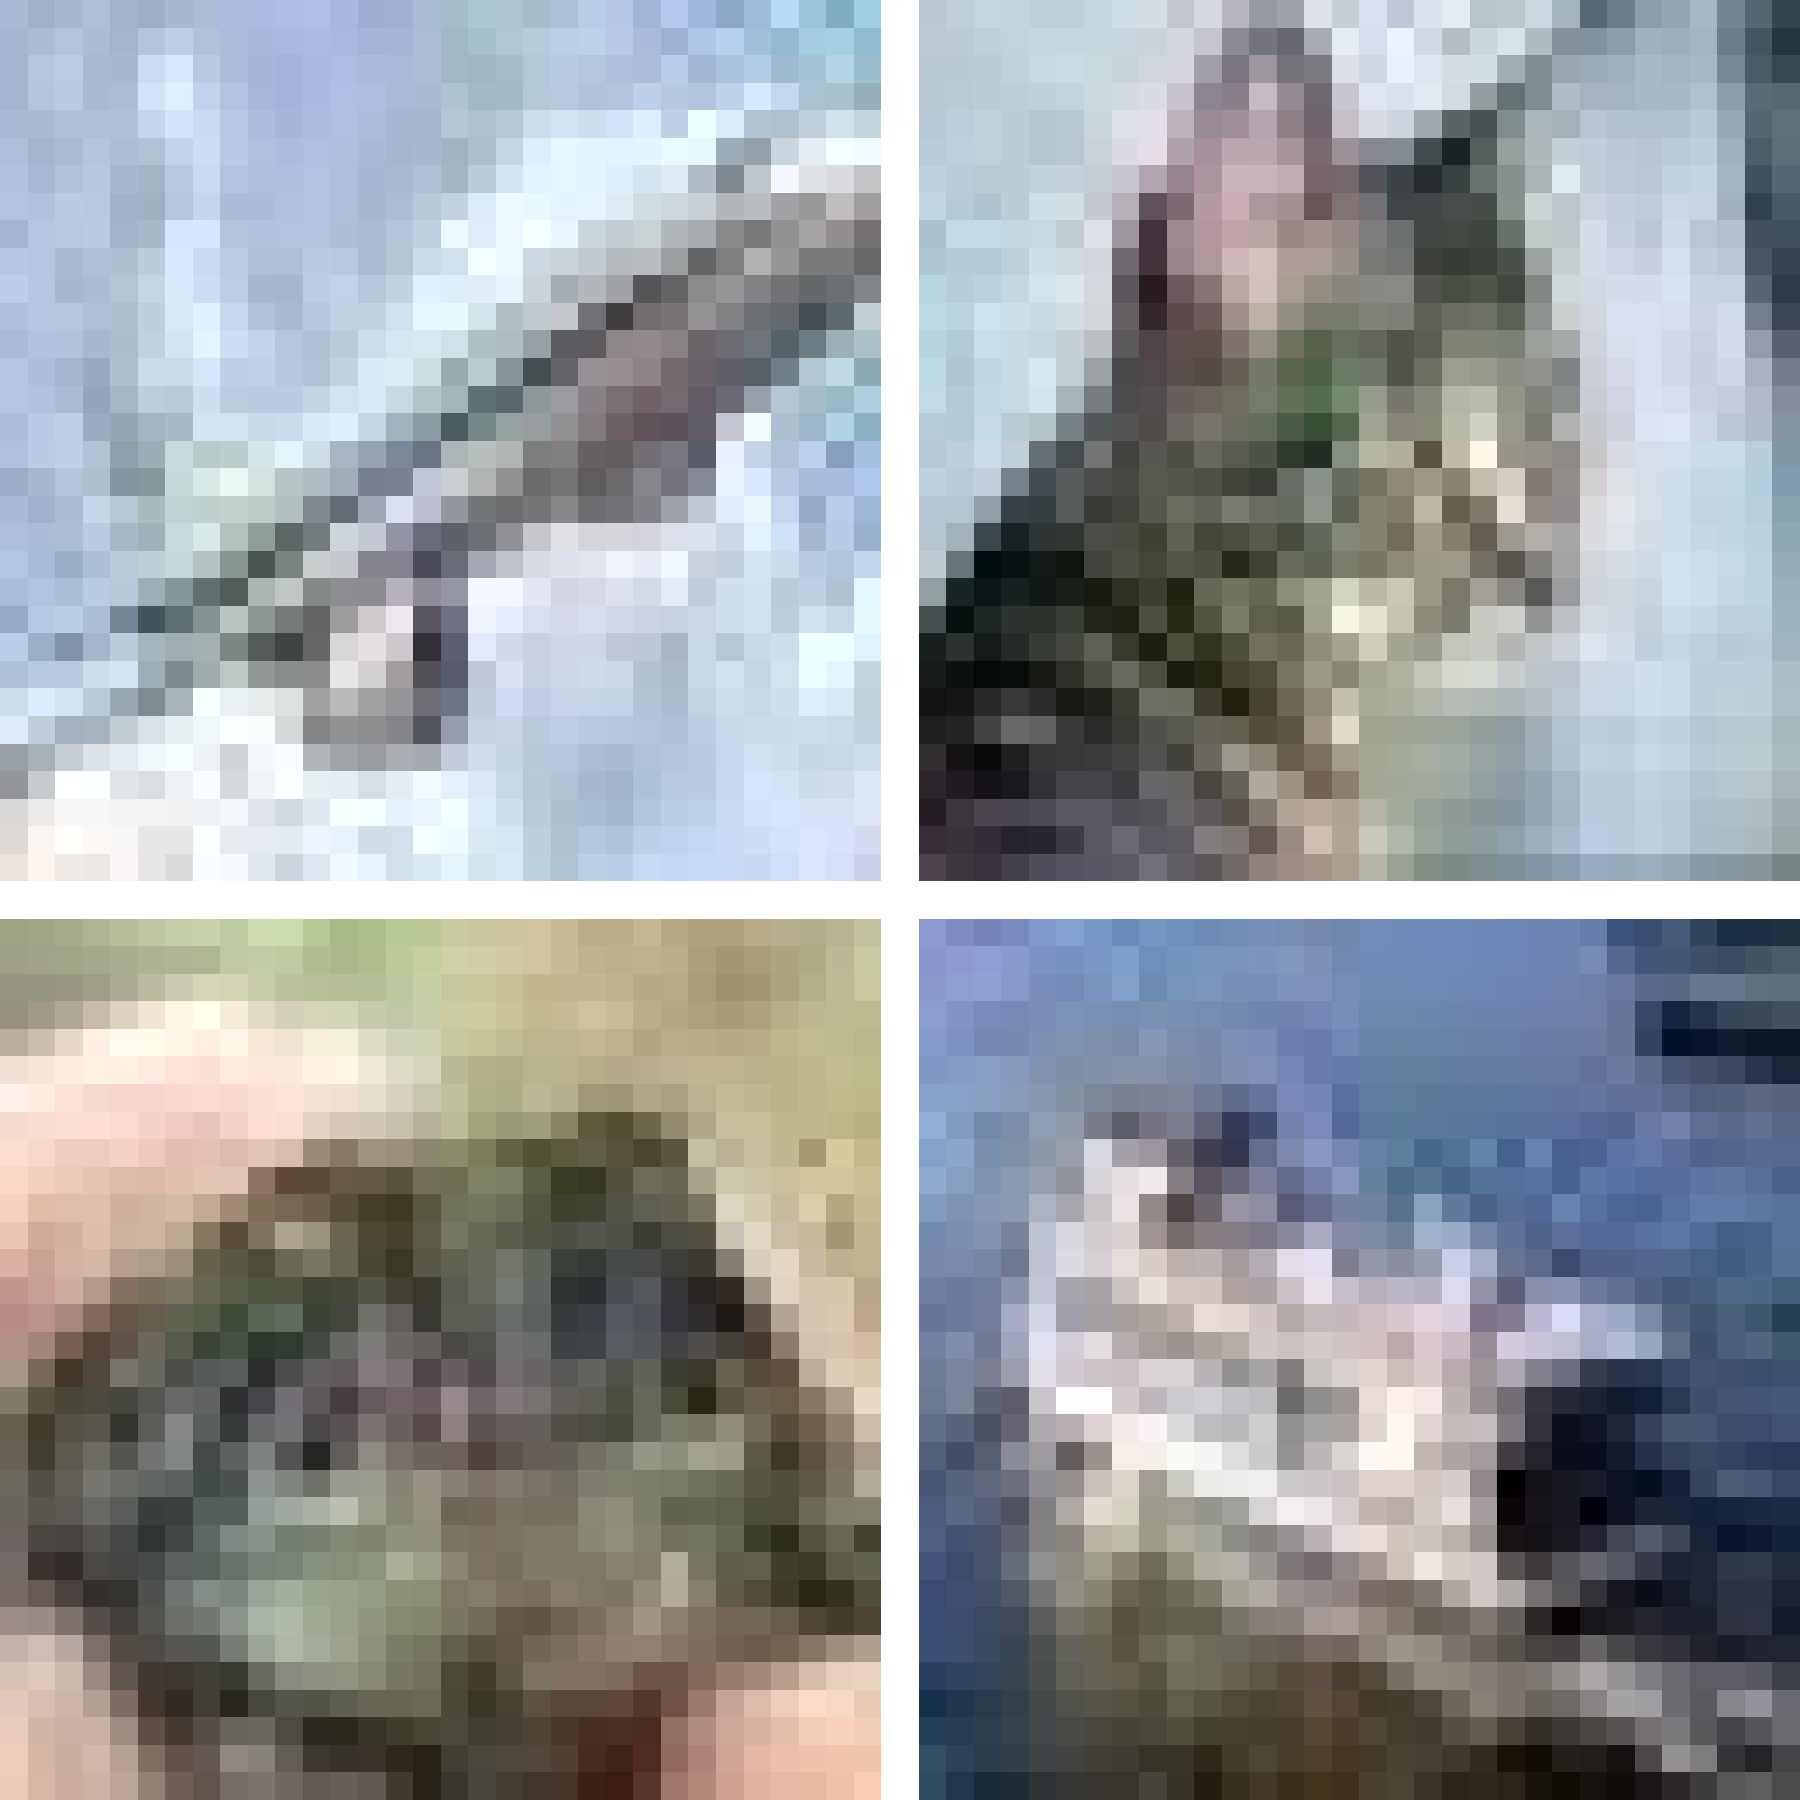
\includegraphics[width=\textwidth]{\toplevelprefix/chapters/chapter7/figs/cifar10.pdf}
        \caption{\small Mostre CIFAR10.}
    \end{subfigure}
    \hfill 
    \phantom{}

    \caption{\small\textbf{Imagini din ImageNet-1K \textit{(stânga)} și CIFAR-10 \textit{(dreapta)}.} Observați că imaginile CIFAR-10 au o rezoluție mult mai mică, în general vorbind, reducând complexitatea învățării acelei distribuții.}
    \label{fig:in1k_cifar10_examples}
\end{figure}

La un nivel puțin mai formal, datele noastre \(\vX\) vor fi imagini; lăsăm \(\cI\) să fie setul tuturor imaginilor. Deoarece o imagine este o matrice dreptunghiulară de pixeli, iar fiecare pixel are o culoare dată de RGB, CMYK sau alt format de culoare, spunem că o imagine este un element al \(\R^{c \times h \times w}\) --- aici \(c\) este numărul de canale (adică, \(3\) pentru RGB și \(4\) pentru CMYK), \(h\) este înălțimea imaginii și \(w\) este lățimea imaginii. În consecință, setul tuturor imaginilor \(\cI \doteq \bigcup_{c, h, w = 1}^{\infty}\R^{c \times h \times w}\) este setul tuturor acestor date posibile. Din nou, vom folosi această notație în mod repetat.


\subsection{Sarcină și Funcție Obiectiv} \label{sub:contrastive_learning_objective}

Sarcina noastră este să învățăm o reprezentare bună a datelor. Învățarea contrastivă, în general, face acest lucru prin definirea proprietăților imaginii de intrare pe care dorim ca caracteristicile să le reflecte, construind imagini care împărtășesc aceste proprietăți dar variază altele, și stabilind o pierdere care promovează că caracteristicile imaginilor cu proprietăți comune sunt apropiate și imaginile cu proprietăți diferite sunt diferite. Soluția naturală optimă la această problemă de învățare este că caracteristicile învățate păstrează proprietățile dorite ale intrării. Cu toate acestea, există multe complicații practice și empirice care apar în cursul antrenării modelelor contrastive.

În cazul DINO, autorii propun să folosească o metodologie care produce un singur vector de caracteristici pentru întreaga imagine și dorește ca vectorul de caracteristici să conțină informații „globale" (adică, la nivel de imagine). În consecință, pierderea va promova că imaginile cu informații globale similare au caracteristici similare și imaginile cu informații globale diferite au caracteristici diferite.

Acest lucru pare intuitiv, dar așa cum am menționat anterior, există mai multe considerații empirice, chiar și în timpul configurării pierderii. În primul și în primul rând, cum ar trebui să promovăm similaritățile și diferențele? Răspunsul de la DINO \citep{caron2021emerging} este\footnote{În opinia autorului, inexplicabil...} să convertească caracteristicile de ieșire în „logit-uri" corespunzătoare unei distribuții de probabilitate și să ia entropia încrucișată a acestora. Mai specific, fie \(\Delta_{m} \doteq \{\vx \in \R^{m} \colon x_{i} \geq 0\ \forall i \in [m], \sum_{i = 1}^{m}x_{i} = 1\}\) spațiul vectorilor de probabilitate în \(\R^{m}\) și definim funcția \(d_{\CE} \colon \R^{m} \times \R^{m} \to \R\) prin
 \begin{equation}\label{eq:cross_entropy_difference}
    d_{\CE}(\vp, \vq) \doteq \CE(\vp, \vq), \quad \forall \vp, \vq \in \Delta_{m}
 \end{equation}
 unde \(\CE \colon \Delta_{m} \times \Delta_{m} \to \R\) este entropia încrucișată, definită ca 
 \begin{equation}\label{eq:expts_def_ce}
    \CE(\vp, \vq) \doteq -\sum_{i = 1}^{m}p_{i}\log q_{i}, \quad \forall \vp = (p_{1}, \dots, p_{m}), \vq = (q_{1}, \dots, q_{m}) \in \Delta_{m}.
 \end{equation}
 Înainte de a continua discuția noastră, să construim o intuiție despre această funcție de distanță. Avem, în particular,
 \begin{align}
    \CE(\vp, \vq)
    &= -\sum_{i = 1}^{m}p_{i}\log q_{i} = \sum_{i = 1}^{m}p_{i}\log(p_{i}/q_{i})
     - \sum_{i = 1}^{m}p_{i}\log p_{i} = \KL(\vp\mmid \vq) + H(\vp)
 \end{align}
 unde \(\KL \colon \Delta_{m} \times \Delta_{m} \to \R\) este divergența KL, definită ca 
 \begin{equation}
    \KL(\vp\mmid \vq) \doteq \sum_{i = 1}^{m}p_{i}\log(p_{i}/q_{i}),
 \end{equation}
 și \(H \colon \Delta_{m} \to \R\) este entropia unei variabile aleatoare. Observați
 că \(\KL(\vp\mmid \vq)\) este minimizată dacă și numai dacă \(\vp = \vq\). Deci minimizarea \(d_{\CE}\) face două lucruri: face \(\vp = \vq\), și face \(\vp\) și \(\vq\) să aibă entropie minimă (adică, vectori cu \(1\) într-o componentă și \(0\) în altă parte --- aceștia se numesc \textit{vectori one-hot}). În general, scopul acestui obiectiv nu este \textit{doar} să potrivească \(\vp\) și \(\vq\), ci și să le modeleze într-un anumit mod pentru a le face cu entropie scăzută. Păstrați acest lucru în minte când discutăm formularea.

Următoarea întrebare este, cum ar trebui să obținem mostre cu informații globale similare? Răspunsul de la DINO (precum și aproape toată învățarea contrastivă) este \textit{augmentarea datelor} --- din fiecare mostră, facem mai multe mostre corelate care împărtășesc proprietățile dorite. În cazul DINO, folosim diferite decupări sau \textit{vederi} ale imaginii de intrare. Amintiți-vă că modelăm o imagine ca un element al setului \(\cI\). În această notație, o vedere este o funcție \(v \colon \cI \to \cI\). În cazul DINO, vederea este o \textit{decupare redimensionată aleatorie}: ia o decupare dreptunghiulară aleasă aleatoriu a imaginii (care are un procent fix \(p_{v} \in [0, 1]\) din suprafața totală a imaginii), o redimensionează proporțional astfel încât \textit{marginea mai scurtă} să aibă \(S_{\rsz}\) pixeli lungime, apoi o redimensionează la o formă fixă \((C, S_{v}, S_{v})\) unde \(S_{v} \geq 1\) este dimensiunea vederii și \(C\) este numărul de canale din imaginea originală.

\begin{figure}
    \centering 
    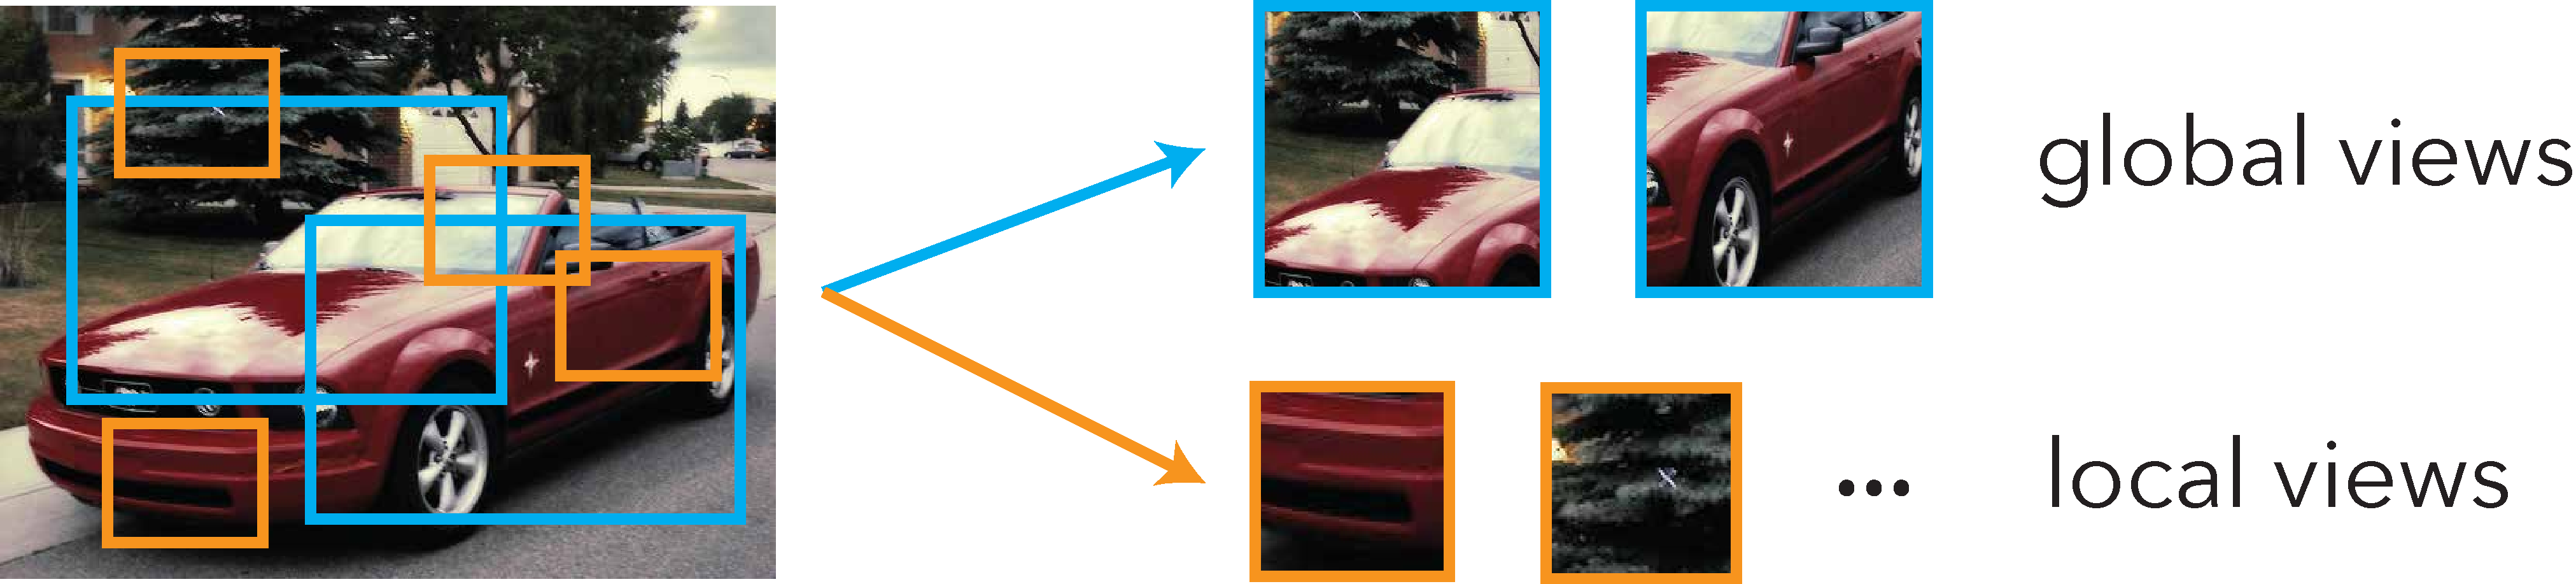
\includegraphics[width=0.7\textwidth]{\toplevelprefix/chapters/chapter7/figs/global_local_views.pdf}
    \caption{\textbf{Vederi locale și globale în DINO.} Vederile locale și vederile globale iau o decupare dreptunghiulară a imaginii de intrare și o redimensionează la o formă pătrată, care este apoi introdusă în rețea pentru procesare.}
    \label{fig:dino_local_global_views}
\end{figure}

Există două tipuri de vederi pe care vrem să le folosim, ilustrate în \Cref{fig:dino_local_global_views}: 
\begin{itemize}
    \item \textit{vederi globale}, care sunt decupări redimensionate aleatorii cu parametru de procent de suprafață \(p_{\glo} \in [0, 1]\) și formă de ieșire \((C, S_{\glo}, S_{\glo})\);
    \item \textit{vederi locale}, care sunt decupări redimensionate aleatorii cu parametru de procent de suprafață \(p_{\loc} \in [0, 1]\) și formă de ieșire \((C, S_{\loc}, S_{\loc})\). Aici \(p_{\loc} < p_{\glo}\) și \(S_{\loc} < S_{\glo}\).
\end{itemize}

DINO dorește ca caracteristicile agregate \(\vz_{\theta}(\vX_{v}) \doteq (f_{\theta}^{\ext} \circ f_{\theta})(\vX_{v})\) ale tuturor vederilor \(\vX_{v} \doteq v(\vX)\) ale unei imagini de intrare \(\vX\) să fie consistente între ele. DINO face acest lucru folosind un \textit{„cap DINO"}\footnote{Observați că \(h_{\vW, \vmu}\) este capul specific sarcinii, care în \Cref{sec:experiment_setup} este parametrizat doar de \(\theta\) spre deosebire de orice parametri specifici, dar deoarece folosim două invocări ale lui \(h\) cu valori diferite ale celui de-al doilea parametru, păstrăm notația specificată.} \(h_{\vW, \vmu}\), parametrizat de o matrice \(\vW \in \R^{s \times d}\) și un vector \(\vmu \in \R^{s}\), pentru a extrage un vector de probabilitate \(\vp_{\theta, \vW, \vmu}(\vX_{v}) \doteq h_{\vW, \vmu}(\vz_{\theta}(\vX_{v}))\) din caracteristica agregată \(\vz_{\theta}(\vX_{v})\), folosind următoarea rețetă simplă:
\begin{equation}
    h_{\vW, \vmu}(\vz) \doteq \softmax([\vW\vz - \vmu]/\tau), \qquad \forall \vz \in \R^{d},
\end{equation}
unde funcția \(\softmax \colon \R^{s} \to \Delta_{s}\) este definită de 
\begin{equation}
    \softmax\rp{\mat{x_{1} \\ \vdots \\ x_{s}}} \doteq \frac{1}{\sum_{i = 1}^{s}e^{x_{i}}}\mat{e^{x_{1}} \\ \vdots \\ e^{x_{s}}}
\end{equation}
și \(\tau > 0\) este un parametru de „temperatură" care controlează entropia ieșirii softmax.

În special, DINO minimizează diferența dintre vectorul de probabilitate \(\vp_{\theta, \vW, \vmu}(\vX_{g}) \doteq h_{\vW, \vmu}(\vz_{\theta}(\vX_{g}))\) pentru fiecare vedere globală \(\vX_{g} \doteq v_{g}(\vX)\) și vectorul de probabilitate \(\vp_{\theta, \vW}(\vX_{c}) \doteq h_{\vW, \vzero_{m}}(\vz_{\theta}(\vX_{c}))\) pentru fiecare vedere \(\vX_{c} \doteq v_{c}(\vX)\). Aici, \(v_{c}\) poate fi \textit{fie} o vedere locală sau o vedere globală. Vom discuta implementarea lui \(f_{\theta}\) și \(f_{\theta}^{\ext}\) în curând în \Cref{sub:contrastive_learning_architecture}. În general, DINO rezolvă problema
 \begin{equation}\label{eq:dino_loss}
     \min_{\theta, \vW, \vmu}\cL_{\dino}(\theta, \vW, \vmu) \qquad \text{unde} \qquad \cL_{\dino}(\theta, \vW, \vmu) \doteq \Ex[d_{\CE}(\vp_{\theta, \vW, \vmu}(\vX_{g}), \vp_{\theta, \vW}(\vX_{c}))],
\end{equation}
unde așteptarea este peste date \(\vX\), vederi globale \(v_{g}\), și alte vederi \(v_{c}\).

În acest caz specific, totuși, dacă încercați să implementați \eqref{eq:dino_loss} și să o optimizați pe o rețea reală, este foarte probabil să întâmpinați o problemă: după rularea câtorva iterații ale algoritmului de învățare, maparea caracteristicilor \(f_{\theta}^{\ext} \circ f_{\theta}\) va \textit{deveni funcția constantă}! Acest lucru optimizează cu siguranță pierderea de mai sus, deoarece minimizează distanța dintre caracteristicile diferitelor vederi ale aceleiași imagini. Dar evident nu vrem să învățăm această soluție.

De fapt, evitarea colapsului este o considerație foarte comună în învățarea contrastivă. Deci, cum o facem în acest caz? Soluția de la DINO, din nou, este proiectată empiric și ajustează cu atenție optimizarea parametrului \(\vmu\) (care este actualizat folosind toate mostrele din lot) și un hiperparametru de „temperatură" \(\tau\) care face parte din implementarea lui \(h_{\vW, \vmu}\) și este discutat în \Cref{sub:contrastive_learning_architecture}. Dat un anumit set special de hiperparametri care funcționează bine, acest lucru este într-adevăr suficient pentru a asigura ne-colapsul reprezentării. Cu toate acestea, în afara acestei configurații speciale, antrenarea modelelor pentru a converge este dificilă, iar antrenamentul este foarte instabil.

Pentru a remedia această stare de lucruri, să discutăm simplificări ale formulării. În primul rând, în loc să calculăm un vector de probabilitate folosind o transformare învățată \(h_{\vW, \vmu}\) a caracteristicilor agregate \(\vz_{\theta}\), putem \textit{folosi direct reprezentarea agregată}, ignorând capul specific sarcinii (sau echivalent, setându-l la maparea identitate). Dar acum avem nevoie de o modalitate de a compara vectorii direct. Folosind ipoteza noastră din \Cref{ch:representation} că reprezentările bune ar trebui să aibă geometrie euclidiană (de subspațiu), o măsură mult mai naturală a diferenței este \textit{distanța \(\ell^{2}\) la pătrat} \(d_{\ell^{2}} \colon \R^{d} \times \R^{d} \to \R\), definită ca 
\begin{equation}\label{eq:cosine_similarity}
    d_{\ell^{2}}(\vx, \vy) \doteq \frac{1}{2}\norm{\vx - \vy}_{2}^{2}, \qquad  \forall \vx, \vy \in \R^{d}.
\end{equation}
Acest scor bazat pe distanță este chiar mai eficient de calculat decât scorul de entropie încrucișată. Astfel, \(d_{\ell^{2}}\) ia locul lui \(d_{\CE}\) în simplificarea noastră.

Înainte, colapsul era evitat folosind trucuri pentru a actualiza \(\vmu\) și \(\tau\). În simplificarea noastră, dacă comparăm caracteristicile în spațiul de reprezentare în loc să le convertim în probabilități, nu avem niciunul dintre acești parametri și astfel trebuie să considerăm o modalitate diferită de a evita colapsul. Pentru a face acest lucru, ne întoarcem la fundamente. Ideea de bază a evitării colapsului este că, pentru a ne asigura că toate mostrele nu returnează exact aceleași caracteristici, avem nevoie ca mostre diferite să aibă caracteristici diferite. Cu alte cuvinte, am dori ca \textit{covarianța} caracteristicilor să fie \textit{mare} într-un anumit sens. Dar din \Cref{ch:compression,ch:representation}, avem deja o cantitate care măsoară dimensiunea matricei de covarianță. Anume, folosim rata directă (la nivel de populație) \textit{de codare Gaussiană} \(R\) pentru a ne asigura că caracteristicile vederilor globale ale diferitelor imagini, care au informații globale diferite, sunt bine separate și nu colapsate (deci extinse). Pierderea generală modificată \(\cL_{\simdino}\) devine:
\begin{equation}\label{eq:simdino_loss}
    \cL_{\simdino}(\theta) \doteq \Ex[d_{\ell^{2}}(\vz_{\theta}(\vX_{g}),
    \vz_{\theta}(\vX_{c}))] - \frac{\gamma}{2}\log\det\rp{\vI + \frac{d}{\eps^{2}}\Cov(\vz_{\theta}(\vX_{g}))},
\end{equation}
unde \(\eps > 0\) este fix și așteptările corespunzătoare sunt, ca înainte, luate peste date \(\vX\), vedere globală \(v_{g}\), și altă vedere (locală sau globală) \(v_{c}\). Pierderea din \eqref{eq:simdino_loss} este pierderea folosită pentru DINO simplificat („SimDINO"). Așa cum vom vedea, când este implementat corespunzător, funcționează cel puțin la fel de bine ca DINO original.

\subsection{Arhitectură: Vision Transformer}\label{sub:contrastive_learning_architecture}

Pentru arhitectură, folosim un transformer de viziune standard. Iată cum funcționează formal o astfel de arhitectură în contextul datelor de imagine. Amintiți-vă din \Cref{sec:experiment_setup} că există patru componente pentru o arhitectură encoder, și anume o încorporare, o coloană vertebrală, un extractor de caracteristici și un cap specific sarcinii. Discutăm aceste patru părți în prezent.

\begin{figure}
    \centering 
    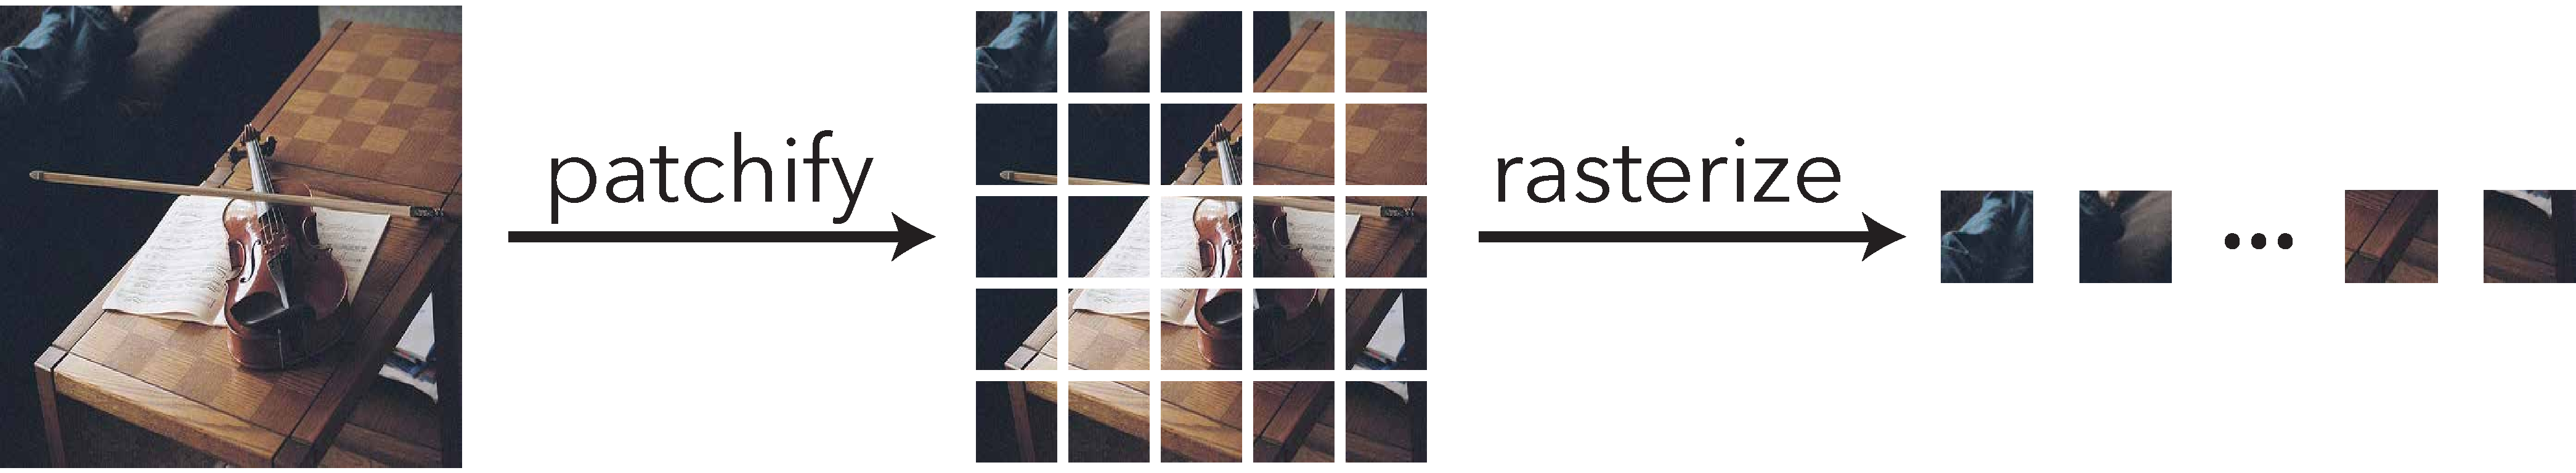
\includegraphics[width=0.8\textwidth]{\toplevelprefix/chapters/chapter7/figs/patchify.pdf}
    \caption{\small\textbf{Un exemplu de imagine transformată în patch-uri pătrate \(5 \times 5\), care sunt plasate în ordine raster.} Fiecare patch are aceeași dimensiune, iar grila de patch-uri are forma \((N_{H}, N_{W}) = (5, 5)\). Grila de patch-uri este apoi desfășurată într-o secvență de lungime \(5 \times 5 = 25\) în ordine raster.}
    \label{fig:patchify_rasterize}
\end{figure}

\begin{figure}
    \centering 
    
\includegraphics[width=\textwidth]{\toplevelprefix/chapters/chapter7/figs/transformer_embedding.pdf}
    \caption{\small\textbf{Pipeline-ul de încorporare transformer.} Dată o secvență de patch-uri desfășurate în ordine raster \(\vX^{\patch}\), fiecare patch desfășurat este proiectat liniar în spațiul caracteristicilor și echipat cu o codare pozițională (aditivă) și un token suplimentar cunoscut ca token de clasă. Ieșirea este caracteristica de intrare în primul strat \(\vZ_{\theta}^{1}(\vX) = f_{\theta}^{\emb}(\vX)\).}
    \label{fig:transformer_embedding}
\end{figure}

\paragraph{Încorporare.} Date fiind datele de imagine \(\vX \in \cI\), le încorporăm ca o secvență de token-uri în \(\R^{d}\) folosind harta \(f_{\theta}^{\emb}\), după cum urmează. Primii doi pași sunt ilustrați în \Cref{fig:patchify_rasterize}, iar ultimii doi sunt ilustrați în \Cref{fig:transformer_embedding}.
\begin{enumerate}
    \item Mai întâi, transformăm datele de imagine \(\vX\) într-o secvență de patch-uri de formă \((C, P_{H}, P_{W})\) unde \(P_{H}\) și \(P_{W}\) sunt dimensiunile patch-urilor. Presupunem că \(P_{H}\) și \(P_{W}\) împart în mod egal înălțimea și lățimea lui \(\vX\), respectiv (în notația din \Cref{sub:contrastive_learning_objective} presupunem că \(P_{H}\) și \(P_{W}\) împart în mod egal \(S_{\loc}\) și \(S_{\glo}\)). Fie grila rezultată de patch-uri să aibă \(N_{H}\) rânduri și \(N_{W}\) coloane.
    \item Desfășurăm fiecare patch într-un vector de lungime \(D \doteq CP_{H}P_{W}\). Există \(N \doteq N_{H}N_{W}\) vectori patch, pe care îi plasăm în „ordine raster" (stânga sus \(\to\) dreapta sus \(\to\) stânga jos \(\to\) dreapta jos) într-o matrice \(\vX^{\patch} \in \R^{D \times N}\), unde \(\vX^{\patch} \doteq f^{\patch}(\vX)\). Observați că \(D\) depinde doar de dimensiunea patch-ului și numărul de canale. Deoarece ultima cantitate este în mod normal constantă între mostrele din același set de date, \(D\) este același pentru toate imaginile din setul de date, în timp ce \(N\) este diferit pentru imagini mai mari și mai mici.
    \item Apoi efectuăm următoarea operație pe \(\vX^{\patch} \in \R^{D \times N}\) pentru a o proiecta la \(\R^{d \times n}\) unde \(n \doteq N + 1\):
    \begin{equation}
        \vX^{\patch} \mapsto [\vz_{\cls}^{1}, \vW^{\emb}\vX] + \vE^{\pos}.
    \end{equation}
    Aici avem trei parametri antrenabili \(\vW^{\emb}\), \(\vz_{\cls}^{1}\), și \(\vE^{\pos}\) al căror scop este următorul:
    \begin{itemize}
        \item \(\vW^{\emb} \in \R^{d \times D}\) este o matrice care proiectează fiecare vector patch la o caracteristică token.
        \item \(\vz_{\cls}^{1} \in \R^{d}\) este un așa-numit \textit{token de clasă} sau \textit{token registru}. Token-ul de clasă deține euristic informații globale despre toate datele și este folosit pentru sarcini în aval. În cadrul rețelelor profunde compresive din \Cref{ch:representation}, ne așteptăm ca token-ul de clasă să fie proiectat pe aceleași subspații ca token-urile saliente sau semantic relevante în timpul progresiei trecerii înainte.
        \item \(\vE^{\pos} \in \R^{d \times N}\) este o așa-numită \textit{codare pozițională} care distinge token-urile diferitelor patch-uri unul de celălalt. Adică, caracteristicile token ar trebui să aibă informații poziționale, astfel încât harta generală \(f^{\pre}\) să nu fie invariantă la permutările patch-urilor, iar \(\vE^{\pos}\) inserează aceste informații poziționale. 
        \begin{itemize}
            \item În acest caz DINO, unde transformerul primește imagini de dimensiuni diferite, învățăm o codare pozițională pentru cea mai mare dimensiune primită în timpul antrenamentului și interpolăm pentru a obține codările poziționale pentru intrările de dimensiuni mai mici.
        \end{itemize}
    \end{itemize}
\end{enumerate}
Astfel, în final avem 
\begin{equation}\label{eq:definition_of_embedding_module}
    f_{\theta}^{\emb}(\vX) \doteq \mat{\vz_{\cls}^{1}, \vW^{\emb}f^{\patch}(\vX) + \vE^{\pos}}.
\end{equation}
Toți parametrii \(\vz_{\cls}^{1}, \vW^{\emb}, \vE^{\pos}\) sunt conținuți în setul de parametri \(\theta\).

\begin{figure}
    \centering 
    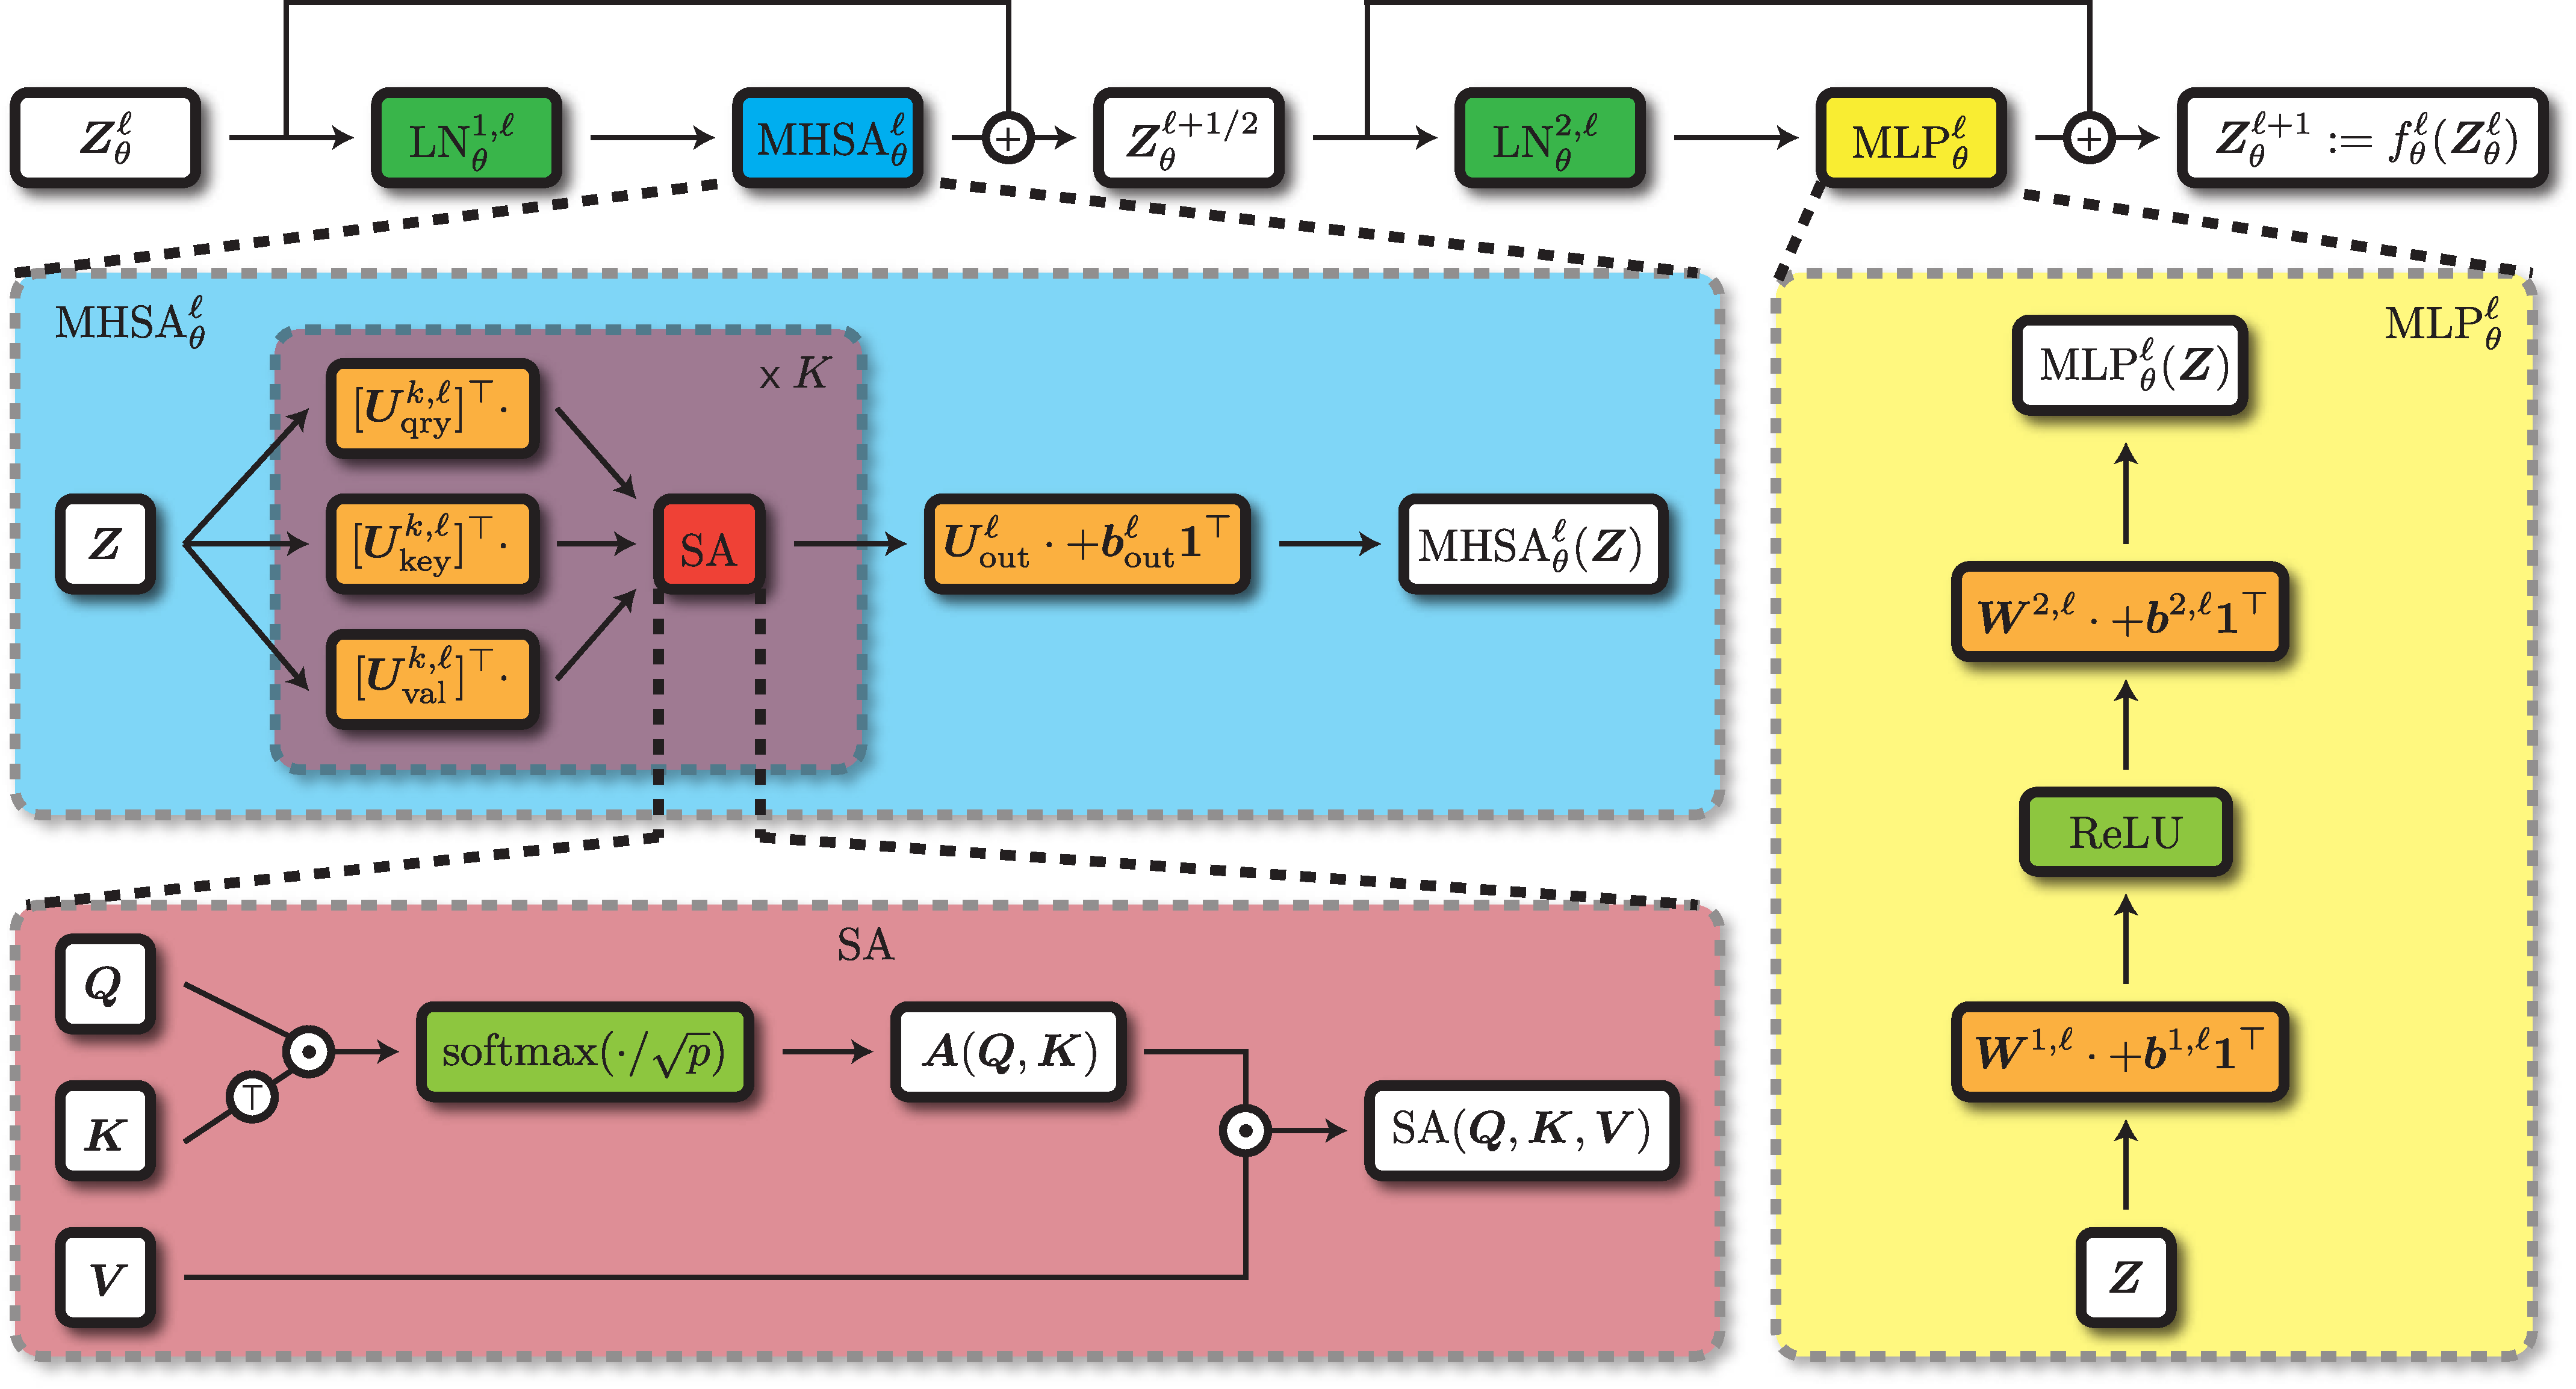
\includegraphics[width=\textwidth]{\toplevelprefix/chapters/chapter7/figs/transformer_backbone.pdf}
    \caption{\small\textbf{Un strat \(f_{\theta}^{\ell}\) al coloanei vertebrale transformer.} Caracteristicile de intrare trec prin blocuri de normalizare de strat, auto-atenție multi-cap și perceptron multi-strat în secvență pentru a forma caracteristicile de ieșire ale stratului.}
    \label{fig:transformer_backbone}
\end{figure}

\paragraph{Coloană vertebrală.} Dată o secvență de încorporări \(\vZ_{\theta}^{1}(\vX) \doteq f_{\theta}^{\emb}(\vX) \in (\R^{d})^{*}\), o procesăm folosind harta coloană vertebrală \(f_{\theta}^{\backbone}\) după cum urmează și așa cum este ilustrat în \Cref{fig:transformer_backbone}. Funcția \(f_{\theta}^{\backbone}\) este compusă din \(L\) \textit{straturi} \(f_{\theta}^{\ell}\), adică,
\begin{equation}
    f_{\theta}^{\backbone} = f_{\theta}^{L} \circ \cdots \circ f_{\theta}^{1}.
\end{equation}
Stratul \(f_{\theta}^{\ell}\) are următoarea implementare:
\begin{align}\label{eq:vit-res-block}
    \vZ_{\theta}^{\ell + 1/2}(\vX)
    &= \vZ_{\theta}^{\ell}(\vX) + \MHSA_{\theta}^{\ell}(\LN_{\theta}^{1, \ell}(\vZ_{\theta}^{\ell}(\vX))) \\ 
    \vZ_{\theta}^{\ell + 1}(\vX)
    &= \vZ_{\theta}^{\ell + 1/2}(\vX) + \MLP_{\theta}^{\ell}(\LN_{\theta}^{2, \ell}(\vZ_{\theta}^{\ell + 1/2}(\vX)))
\end{align}
și \(f_{\theta}^{\ell}\) este definit astfel încât \(f_{\theta}^{\ell}(\vZ_{\theta}^{\ell}(\vX)) \doteq \vZ_{\theta}^{\ell + 1}(\vX)\). Aici am folosit câțiva operatori, cum ar fi \(\MHSA_{\theta}^{\ell}, \MLP_{\theta}^{\ell}\) și \(\LN_{\theta}^{i, \ell}\) care sunt definiți după cum urmează:
\begin{itemize}
    \item Operatorul \(\MHSA_{\theta}^{\ell}\) este auto-atenție multi-cap, predecesorul auto-atenției de subspațiu multi-cap (cf \Cref{ch:representation}). Formularea este următoarea:
    \begin{align}
        \MHSA_{\theta}^{\ell}(\vZ) \label{eq:mhsa}
        &\doteq \vU_{\out}^{\ell}\mat{\SA([\vU_{\query}^{1, \ell}]^{\top}\vZ, [\vU_{\attnkey}^{1, \ell}]^{\top}\vZ, [\vU_{\val}^{1, \ell}]^{\top}\vZ) \\ \vdots \\ \SA([\vU_{\query}^{K, \ell}]^{\top}\vZ, [\vU_{\attnkey}^{K, \ell}]^{\top}\vZ, [\vU_{\val}^{K, \ell}]^{\top}\vZ)} + \vb_{\out}^{\ell}\vone_{n}^{\top}, \\
        \label{eq:self_attention}
        \text{unde} \qquad \SA(\vQ, \vK, \vV)
        &\doteq \vV \underbrace{\softmax\rp{\frac{\vK^{\top}\vQ}{\sqrt{p}}}}_{\doteq \vA(\vQ, \vK)}
    \end{align}
    unde \(p\) este un întreg pozitiv, \(\vU_{\query}^{k, \ell}, \vU_{\attnkey}^{k, \ell}, \vU_{\val}^{k, \ell} \in \R^{d \times p}\), \(\vU_{\out}^{\ell} \in \R^{d \times Kp}\), și \(\vb_{\out}^{\ell} \in \R^{d}\) sunt parametri antrenabili conținuți în setul de parametri \(\theta\), iar \(\softmax\) este definit pe coloane ca 
    \begin{align}
        \softmax(\vM) 
        &\doteq \mat{\softmax(\vm_{1}) & \cdots & \softmax(\vm_{p})}, \\ 
        \forall \vM 
        &= \mat{\vm_{1}, \dots, \vm_{p}} \in \R^{n \times p}.
    \end{align}
    În practică, dimensiunile sunt de obicei alese astfel încât \(Kp = d\). Termenii 
    \begin{equation}
        \label{eq:attention_map}
        \vA_{\theta}^{k, \ell}(\vZ) \doteq \vA([\vU_{\query}^{k, \ell}]^{\top}\vZ, [\vU_{\attnkey}^{k, \ell}]^{\top}\vZ), \qquad \SA_{\theta}^{k, \ell}(\vZ) \doteq \SA([\vU_{\query}^{k, \ell}]^{\top}\vZ, [\vU_{\attnkey}^{k, \ell}]^{\top}\vZ, [\vU_{\val}^{k, \ell}]^{\top}\vZ)
    \end{equation}
    sunt de asemenea cunoscuți ca \textit{harta de atenție \(k\)} și respectiv \textit{ieșirea capului de atenție \(k\)} la stratul \(\ell\). Mai mult, operația \(\SA(\vQ, \vK, \vV)\) poate fi calculată extrem de eficient folosind software specializat precum FlashAttention \citep{shah2025flashattention}.
    \item \(\MLP_{\theta}^{\ell}\) este un perceptron cu două straturi, o neliniaritate regulată folosită în rețelele profunde, și are forma 
    \begin{equation}
        \MLP_{\theta}^{\ell}(\vZ) \doteq \vW_{\down}^{\ell}\ReLU(\vW_{\up}^{\ell}\vZ + \vb_{\up}^{\ell}\vone_{n}^{\top}) + \vb_{\down}^{\ell}\vone_{n}^{\top}
    \end{equation}
    unde \(\vW_{\up}^{\ell} \in \R^{q \times d}, \vW_{\down}^{\ell} \in \R^{d \times q}, \vb_{\up}^{\ell} \in \R^{q}, \vb_{\down}^{\ell} \in \R^{d}\) sunt parametri antrenabili conținuți de asemenea în setul de parametri \(\theta\), iar \(\ReLU\) este neliniaritatea ReLU element cu element, adică, \(\ReLU(\vM)_{ij} = \max\{M_{ij}, 0\}\). 
    \item Fiecare layer-norm \(\LN_{\theta}^{i, \ell}\) pentru \(i \in \{1, 2\}\) este o normalizare standard, care se aplică pe coloane la fiecare caracteristică token independent:
    \begin{equation}
        \LN_{\theta}^{i, \ell}(\vZ) = \LN_{\theta}^{i, \ell}(\mat{\vz_{1}, \dots, \vz_{n}}) = \mat{\LN_{\theta}^{i, \ell}(\vz_{1}), \dots, \LN_{\theta}^{i, \ell}(\vz_{n})}
    \end{equation}
    și are forma 
    \begin{equation}
        \LN_{\theta}^{i, \ell}(\vz) = \frac{\vz
        - \operatorname{mean}(\vz)\vone_{d}}{\norm{\vz
        - \operatorname{mean}(\vz)\vone_{d}}_{2}} \hada \valpha^{i, \ell} + \vbeta^{i, \ell} \qquad \text{unde} \qquad \operatorname{mean}(\vz) = \frac{1}{d}\vone_{d}^{\top}\vz
    \end{equation}
    unde \(\hada\) denotă înmulțirea element cu element, iar \(\valpha^{i, \ell}, \vbeta^{i, \ell} \in \R^{d}\) sunt parametri antrenabili conținuți în setul de parametri \(\theta\). Operatorul layer-norm servește ca un fel de normalizare pe fiecare token, unde scala fiecărui token după aceea este învățabilă și împărtășită între toate token-urile. 
\end{itemize}

Transformerul este una dintre cele mai populare arhitecturi de rețele neuronale din istorie, alimentând aplicații în aproape toate domeniile învățării profunde.

\paragraph{Extractor de caracteristici.} Folosim un pas de post-procesare \(f_{\theta}^{\ext}\) care extrage \textit{caracteristica token de clasă}, care (amintiți-vă) este caracteristica menită să conțină informații agregate despre imaginea de intrare, și aplică un MLP și normalizare la aceasta. Anume, avem 
\begin{equation}
    \vz_{\theta}(\vX) \doteq f_{\theta}^{\ext}(\vZ_{\theta}(\vX)) = f_{\theta}^{\ext}([\vz_{\theta}^{1}(\vX), \dots, \vz_{\theta}^{n}(\vX)]) \doteq \frac{\MLP_{\theta}^{\ext}(\vz_{\theta}^{1}(\vX))}{\norm{\MLP_{\theta}^{\ext}(\vz_{\theta}^{1}(\vX))}_{2}}.
\end{equation} 

\paragraph{Cap specific sarcinii („DINO").} Pentru DINO, folosim capul DINO specific sarcinii \(h_{\vW, \vmu}\). Pentru SimDINO, nu folosim \textit{niciun} cap specific sarcinii \textit{deloc}, așa cum a fost descris anterior.

\subsection{Strategie de Optimizare}\label{sub:contrastive_learning_optimization}

\begin{figure}
    \centering 
    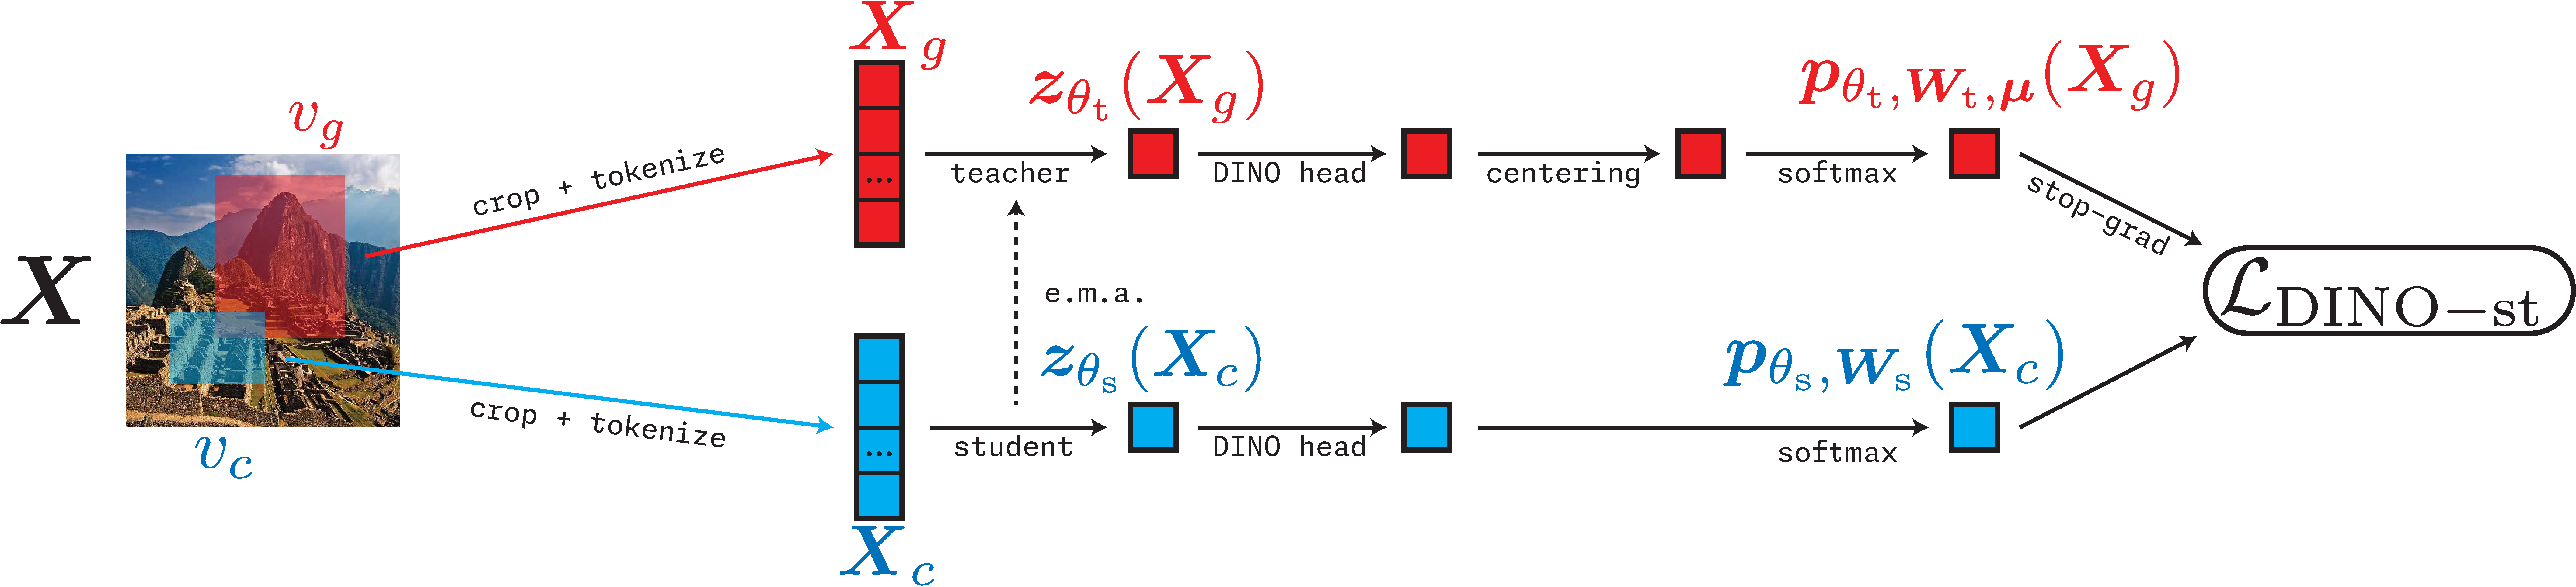
\includegraphics[width=\textwidth]{\toplevelprefix/chapters/chapter7/figs/dino_pipeline.pdf}
    \caption{\small \textbf{Pipeline-ul DINO.} Caracteristicile student și caracteristicile profesor sunt calculate pentru fiecare intrare. Obiectivul încearcă să alinieze caracteristicile student cu caracteristicile profesor prin proiectarea ambelor seturi de caracteristici într-un simplex de probabilitate de dimensiune înaltă și calcularea unei pierderi de entropie încrucișată. În mod notabil, din cauza „stop-grad", gradientul este calculat doar în raport cu \textit{ieșirile parametrilor student}.}
    \label{fig:dino_pipeline}
\end{figure}

\paragraph{Optimizarea DINO.} Avem o funcție de pierdere și o arhitectură, așa că acum discutăm strategia de optimizare. Strategia de optimizare pentru DINO folosește \textit{două seturi de ponderi pentru aceeași arhitectură}: ponderi \textit{student} \(\theta_{\student}\) și ponderi \textit{profesor} \(\theta_{\teacher}\). Acestea corespund la două rețele neuronale diferite, numite rețeaua profesor și rețeaua student, cu aceeași arhitectură. Rețeaua profesor codifică toate vederile globale, în timp ce rețeaua student codifică toate vederile „alte". Scopul pierderii este de a distila ieșirile profesorului în modelul student. Anume, antrenăm pe pierderea \(\cL_{\dino{}-\student\teacher}\):
\begin{equation}\label{eq:dino_loss_teacherstudent}
    \cL_{\dino{}-\student\teacher}(\theta_{\student}, \theta_{\teacher}, \vW_{\student}, \vW_{\teacher}, \vmu) \doteq \Ex[d_{\CE}(\vp_{\theta_{\teacher}, \vW_{\teacher}, \vmu}(\vX_{g}), \vp_{\theta_{\student}, \vW_{\student}}(\vX_{c}))].
\end{equation}
Acum, putem descrie complet pipeline-ul general al DINO, ilustrat în \Cref{fig:dino_pipeline}.

Deși este ușor să raționăm despre \eqref{eq:dino_loss_teacherstudent}, este imposibil în practică să implementăm algoritmi de optimizare cum ar fi gradientul descendent cu o pierdere dată de \(\cL_{\dino{}-\student\teacher}\). Acest lucru se datorează faptului că așteptările din pierdere sunt imposibil de evaluat, cu atât mai puțin de a lua gradientul. În acest caz extrem de frecvent, aproximăm așteptarea prin mostre finite. Adică, la fiecare pas de timp \(k\):
\begin{itemize}
    \item Sub-eșantionăm \(B\) puncte de date din setul nostru de date \(\{\vX_{1}^{(k)}, \dots, \vX_{B}^{(k)}\} \subset \cI\).
    \item Pentru fiecare punct de date \(\vX_{b}^{(k)}\), eșantionăm \(M_{\glo}\) vederi globale \(v_{b, g}^{(k), i}\) și \(M_{\loc}\) vederi locale \(v_{b, \ell}^{(k), i}\). Aplicăm vederile la \(\vX_{b}^{(k)}\) pentru a obține \(\vX_{b, g}^{(k), i} \doteq v_{b, g}^{(k), i}(\vX_{b}^{(k)})\) și \(\vX_{b, \ell}^{(k), i} \doteq v_{b, \ell}^{(k), i}(\vX_{b}^{(k)})\).
    \item Pentru fiecare vedere \textit{locală} \(\vX_{b, \ell}^{(k), i}\), calculăm următoarele cantități:
    \begin{equation}
        \vz_{\theta_{\student}}(\vX_{b, \ell}^{(k), i}) \doteq (f_{\theta_{\student}}^{\ext} \circ f_{\theta_{\student}})(\vX_{b, \ell}^{(k), i}), \qquad \vp_{\theta_{\student}, \vW_{\student}}(\vX_{b, \ell}^{(k), i}) \doteq h_{\vW_{\student}, \vzero_{m}}(\vz_{\theta_{\student}}(\vX_{b, \ell}^{(k), i}(\theta)))
    \end{equation}
    și pentru fiecare vedere \textit{globală} \(\vX_{b, g}^{(k), i}\), calculăm următoarele cantități (prin abuz de notație):
    \begin{align}
        &\vz_{\theta_{\student}}(\vX_{b, g}^{(k), i}) \doteq (f_{\theta_{\student}}^{\ext} \circ f_{\theta_{\student}})(\vX_{b, g}^{(k), i}), \qquad \vp_{\theta_{\student}, \vW_{\student}}(\vX_{b, g}^{(k), i}) \doteq h_{\vW_{\student}, \vzero_{m}}(\vz_{\theta_{\student}}(\vX_{b, g}^{(k), i})), \\
        &\vz_{\theta_{\teacher}}(\vX_{b, g}^{(k), i}) \doteq (f_{\theta_{\teacher}}^{\ext} \circ f_{\theta_{\teacher}})(\vX_{b, g}^{(k), i}), \qquad \vp_{\theta_{\teacher}, \vW_{\teacher}, \vmu}(\vX_{b, g}^{(k), i}) \doteq h_{\vW_{\teacher}, \vmu}(\vZ_{\theta_{\teacher}}(\vX_{b, g}^{(k), i})).
    \end{align}
    \item Calculăm \textit{pierderea surogat, aproximată} \(\hat{\cL}_{\dino-\student\teacher}^{(k)}\), definită după cum urmează: 
    \begin{align}\label{eq:dino_loss_teacherstudent_empirical}
        &\hat{\cL}_{\dino{}-\student\teacher}^{(k)}(\theta_{\student}, \theta_{\teacher}, \vW_{\student}, \vW_{\teacher}, \vmu) \doteq
        \frac{1}{BM_{\glo}(M_{\glo} + M_{\loc} - 1)}\sum_{b = 1}^{B}\sum_{i = 1}^{M_{\glo}}\\
        &\Bigg[\sum_{j = 1}^{M_{\loc}}d_{\CE}(\vp_{\theta_{\teacher}, \vW_{\teacher}, \vmu}(\vX_{b, g}^{(k), i}), \vp_{\theta_{\student}, \vW_{\student}}(\vX_{b, \ell}^{(k), j})) + \sum_{\substack{j = 1 \\ j \neq i}}^{M_{\glo}}d_{\CE}(\vp_{\theta_{\teacher}, \vW_{\teacher}, \vmu}(\vX_{b, g}^{(k), i}), \vp_{\theta_{\student}, \vW_{\student}}(\vX_{b, g}^{(k), j}))\Bigg]\nonumber
    \end{align}
    precum și gradienții săi în raport cu \(\theta_{\student}\) și \(\vW_{\student}\), care ar trebui calculați sub presupunerea că \(\theta_{\teacher}\), \(\vW_{\teacher}\), și \(\vmu\) sunt constante --- adică că sunt \textit{detașate de graficul computațional} și nu depind de \(\theta_{\student}\) și \(\vW_{\student}\).
    \item Actualizăm parametrii student \(\theta_{\student}\) și \(\vW_{\student}\) prin intermediul unui algoritm de optimizare iterativ bazat pe gradient, și actualizăm \(\theta_{\teacher}\), \(\vW_{\teacher}\), și \(\vmu\) prin medii mobile exponențiale cu parametri de decay \(\nu^{(k)}\), \(\nu^{(k)}\), și \(\rho^{(k)}\) respectiv, adică, 
    \begin{align}
        (\theta_{\student}^{(k + 1)}, \vW_{\student}^{(k + 1)})
        &= \textsc{OptUpdate}^{(k)}(\theta_{\student}^{(k)}, \vW_{\student}^{(k)}; \nabla_{(\theta_{\student}, \vW_{\student})}\hat{\cL}_{\dino-\student\teacher}^{(k)}) \\
        \theta_{\teacher}^{(k + 1)}
        &= \nu^{(k)}\theta_{\teacher}^{(k)} + (1 - \nu^{(k)})\theta_{\student}^{(k + 1)} \\
        \vW_{\teacher}^{(k + 1)}
        &= \nu^{(k)}\vW_{\teacher}^{(k)} + (1 - \nu^{(k)})\vW_{\student}^{(k + 1)} \\
        \vmu^{(k + 1)}
        &= \rho^{(k)}\vmu^{(k)} + (1 - \rho^{(k)})\cdot\frac{1}{BM_{\glo}}\sum_{b = 1}^{B}\sum_{i = 1}^{M_{\glo}}\vW^{(k)}\vz_{\theta_{\teacher}}(\vX_{b, g}^{(k), i}),
    \end{align}
    De exemplu, dacă algoritmul de optimizare ales ar fi gradientul descendent stocastic, am avea actualizarea \(\theta_{\student}^{(k + 1)} \doteq \theta_{\student}^{(k)} - \delta^{(k)}\nabla_{\theta_{\student}}\hat{\cL}_{\dino{}-\student\teacher}^{(k)}\), și așa mai departe.
\end{itemize}
Observați că procedura de optimizare este destul de neregulată: deși toți cei patru parametri se schimbă la fiecare iterație, doar doi dintre ei sunt actualizați direct dintr-o metodă bazată pe gradient. Ceilalți doi sunt actualizați din medii mobile exponențiale și într-adevăr tratați ca constante când se calculează orice gradienți. După antrenament, aruncăm ponderile student și folosim ponderile profesor pentru rețeaua noastră antrenată \(f\), deoarece această medie mobilă exponențială s-a dovedit empiric că stabilizează modelul rezultat (această idee este cunoscută ca medierea Polyak sau medierea iterațiilor).

Modul în care \(\nu\) și \(\rho\) se schimbă de-a lungul traiectoriei de optimizare (adică, funcțiile \(k \mapsto \nu^{(k)}\) și \(k \mapsto \rho^{(k)}\)) sunt hiperparametri sau decizii de design, cu \(\nu^{(1)} < 1\) și \(\lim_{k \to \infty}\nu^{(k)} = 1\) de obicei, și similar pentru \(\rho\). Hiperparametrul de temperatură \(\tau\), folosit în capul DINO \(h_{\vW, \vmu}\), se schimbă de asemenea de-a lungul traiectoriei de optimizare (deși această dependență nu este notată explicit).

Folosirea pierderii surogat („empirice") transformă problema noastră de optimizare intractabilă, ca în optimizarea pierderii din \eqref{eq:dino_loss_teacherstudent}, într-o problemă de optimizare stocastică tractabilă care este rulată pentru a antrena în esență fiecare model de învățare profundă din lume. Această conversie este extrem de naturală odată ce ați văzut câteva exemple, și sperăm să oferim aceste exemple pe parcursul capitolului.

\begin{figure}
    \centering 
    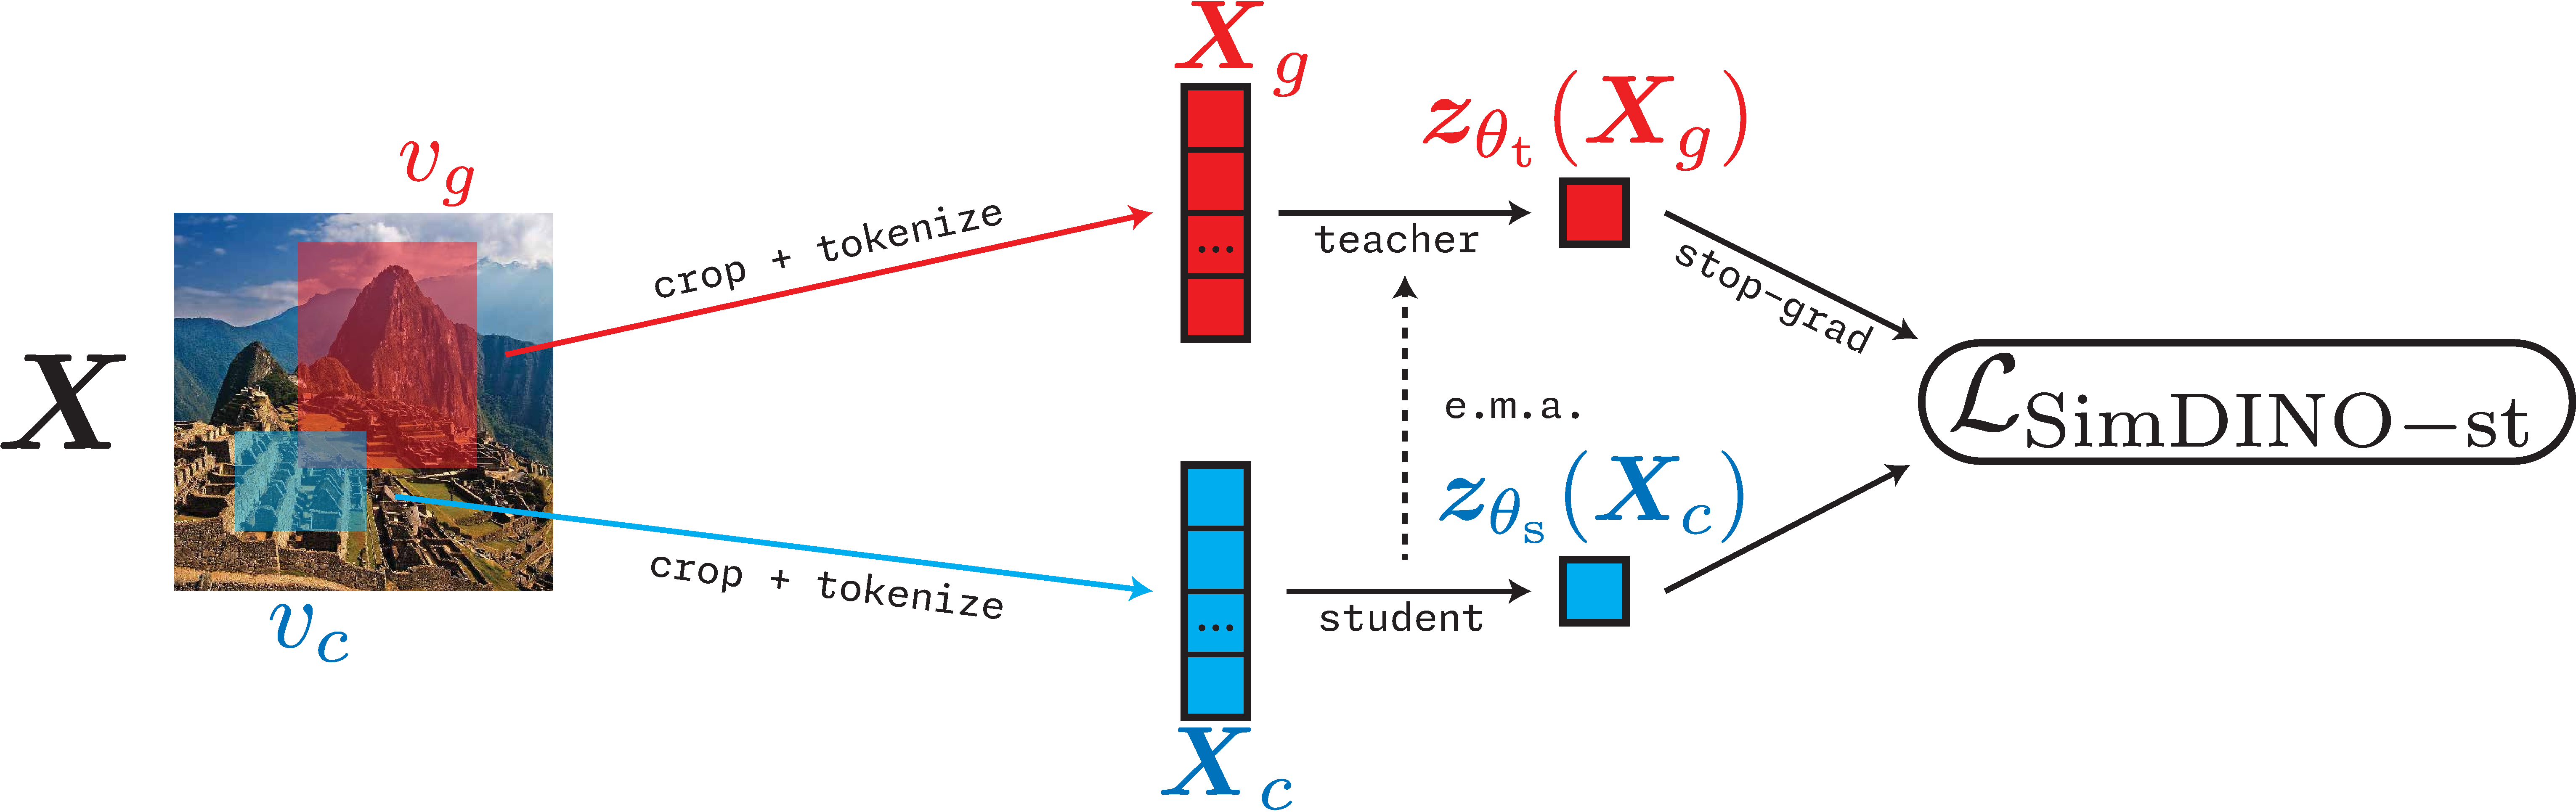
\includegraphics[width=0.7\textwidth]{\toplevelprefix/chapters/chapter7/figs/simdino_pipeline.pdf}
    \caption{\small\textbf{Pipeline-ul SimDINO.} Aici, în contrast cu pipeline-ul DINO din \Cref{fig:dino_pipeline}, pierderea este calculată direct pe caracteristici fără necesitatea unei manipulări suplimentare. Acest lucru elimină parametrii a câtorva matrice mari și simplifică pipeline-ul, făcându-l simultan mai stabil de antrenat.}\label{fig:simdino_pipeline}
\end{figure}

\paragraph{Optimizarea SimDINO.} Obiectivul la nivel de populație DINO simplificat este foarte similar în spirit, dar mult mai simplu în execuție, adică,
\begin{equation}\label{eq:simdino_loss_teacherstudent}
    \cL_{\simdino-\student\teacher}(\theta_{\student}, \theta_{\teacher}) \doteq
    \Ex\rs{d_{\ell^{2}}(\vz_{\theta_{\teacher}}(\vX_{g}),
    \vz_{\theta_{\student}}(\vX_{c}))} - \frac{\gamma}{2}\log\det\rp{\vI + \frac{d}{\eps^{2}}\Cov(\vz_{\theta_{\student}}(\vX_{g})))}.
\end{equation}
Astfel, așa cum este elaborat în \Cref{fig:simdino_pipeline}, pipeline-ul SimDINO este strict mai simplu decât pipeline-ul DINO. Putem folosi o versiune mai simplă a pipeline-ului de antrenament DINO pentru a optimiza SimDINO. La fiecare pas de timp \(k\):
\begin{itemize}
    \item Sub-eșantionăm \(B\) puncte de date din setul nostru de date \(\{\vX_{1}^{(k)}, \dots, \vX_{B}^{(k)}\} \subset \cI\).
    \item Pentru fiecare punct de date \(\vX_{b}^{(k)}\), eșantionăm \(M_{\glo}\) vederi globale \(v_{b, g}^{(k), i}\) și \(M_{\loc}\) vederi locale \(v_{b, \ell}^{(k), i}\). Aplicăm vederile la \(\vX_{b}^{(k)}\) pentru a obține \(\vX_{b, g}^{(k), i} \doteq v_{b, g}^{(k), i}(\vX_{b}^{(k)})\) și \(\vX_{b, \ell}^{(k), i} \doteq v_{b, \ell}^{(k), i}(\vX_{b}^{(k)})\).
    \item Pentru fiecare vedere \textit{locală} \(\vX_{b, \ell}^{(k), i}\) calculăm \(\vz_{\theta_{\student}}(\vX_{b, \ell}^{(k), i}) \doteq (f_{\theta_{\student}}^{\ext} \circ f_{\theta_{\student}})(\vX_{b, \ell}^{(k), i})\). Pentru fiecare vedere \textit{globală} \(\vX_{b, g}^{(k), i}\) calculăm \(\vz_{\theta_{\student}}(\vX_{b, g}^{(k), i}) \doteq (f_{\theta_{\student}}^{\ext} \circ f_{\theta_{\student}})(\vX_{b, g}^{(k), i})\) și \(\vz_{\theta_{\teacher}}(\vX_{b, g}^{(k), i}) \doteq (f_{\theta_{\teacher}}^{\ext} \circ f_{\theta_{\teacher}})(\vX_{b, g}^{(k), i})\).
    \item Calculăm \textit{pierderea surogat, aproximată} \(\hat{\cL}_{\simdino-\student\teacher}^{(k)}\), definită după cum urmează: 
    \begin{align}\label{eq:simdino_loss_teacherstudent_empirical}
        &\hat{\cL}_{\simdino{}-\student\teacher}^{(k)}(\theta_{\student}, \theta_{\teacher}) \doteq
        \frac{1}{BM_{\glo}(M_{\glo} + M_{\loc} - 1)}\sum_{b = 1}^{B}\sum_{i = 1}^{M_{\glo}}\Bigg[\sum_{j = 1}^{M_{\loc}}d_{\ell^{2}}(\vz_{\theta_{\teacher}}(\vX_{b, g}^{(k), i}), \vz_{\theta_{\student}}(\vX_{b, \ell}^{(k), j})) \\ 
        &\qquad \qquad + \sum_{j = 1}^{M_{\glo}}d_{\ell^{2}}(\vz_{\theta_{\teacher}}(\vX_{b, g}^{(k), i}), \vz_{\theta_{\student}}(\vX_{b, g}^{(k), j}))\Bigg] - \frac{\gamma}{M_{\glo}}\sum_{i = 1}^{M_{\glo}}R_{\eps}([\vz_{\theta_{\student}}(\vX_{1, g}^{(k), i}), \dots, \vz_{\theta_{\student}}(\vX_{B, g}^{(k), i})])\nonumber
    \end{align}
    unde \(R_{\eps}\) este rata de codare Gaussiană estimată pe mostre finite, descrisă în \Cref{ch:representation}. Gradientul lui \(\hat{\cL}_{\simdino-\student\teacher}^{(k)}\) în raport cu \(\theta_{\student}\) ar trebui (din nou) calculat, sub presupunerea că \(\theta_{\teacher}\) este constantă.
    \item Actualizăm parametrii student \(\theta_{\student}\) prin intermediul unui algoritm de optimizare iterativ bazat pe gradient, și actualizăm \(\theta_{\teacher}\) prin intermediul unei medii mobile exponențiale cu parametru de decay \(\nu^{(k)}\), adică, 
    \begin{align}
        \theta_{\student}^{(k + 1)}
        &= \textsc{OptUpdate}^{(k)}(\theta_{\student}^{(k)}; \nabla_{\theta_{\student}}\hat{\cL}_{\simdino-\student\teacher}^{(k)}) \\
        \theta_{\teacher}^{(k + 1)}
        &= \nu^{(k)}\theta_{\teacher}^{(k)} + (1 - \nu^{(k)})\theta_{\student}^{(k + 1)}.
    \end{align}
\end{itemize}
Din nou, reiterăm că gradientul este luat doar în raport cu \(\theta_{\student}\), tratând \(\theta_{\teacher}\) ca o constantă. Aici, observați că, în timp ce alegerea lui \(\nu\) este încă o decizie de design, hiperparametrii \(\rho\) și \(\tau\) sunt eliminați.


\subsection{Metodologie de Evaluare}\label{sub:contrastive_learning_evals}
Există mai multe moduri de a evalua un model transformer antrenat. Evidențiem două în această secțiune. Să definim vederea \textit{decupare centrală} \(v_{\cc} \colon \cI \to \cI\) care este o \textit{decupare redimensionată deterministă}:
\begin{itemize}
    \item redimensionează imaginea astfel încât marginea cea mai scurtă să fie de dimensiune \(S_{\rsz}\) (similar cu decupările redimensionate aleatorii cu parametru de procent de suprafață \(1\));
    \item apoi ia decuparea \textit{centrală} \(S_{\cc} \times S_{\cc}\);
\end{itemize}
astfel încât forma finală este \((C, S_{\cc}, S_{\cc})\). Observați că vederea \(v_{\cc}\) este complet deterministă dată o intrare. Pentru o intrare \(\vX\), scriem \(\vX_{\cc} \doteq v_{\cc}(\vX)\). Aici \(S_{\cc} \leq S_{\rsz}\).


\paragraph{Sondare liniară.}

Primul și cel mai agnostic arhitectural mod de a evalua un model encoder \(\vX \mapsto \vz_{\theta}(\vX)\) este să folosim \textit{sondarea liniară}. Sondarea liniară este, într-o propoziție, rularea regresiei logistice pe caracteristicile agregate calculate de encoder. Acest lucru ne spune câtă informație semantică există în reprezentări, precum și cât de ușor poate fi extrasă această informație. (Adică: în ce măsură caracteristicile imaginilor cu semantici diferite trăiesc pe subspații diferite ale spațiului caracteristicilor?)

Mai formal, să presupunem că vrem să evaluăm calitatea și fidelitatea caracteristicilor encoder-ului pe date imagine-etichetă \((\vX, \vy)\), unde există \(N_{\cls}\) clase și \(\vy \in \{0, 1\}^{N_{\cls}}\) este o „codare one-hot" (adică, zerouri în toate pozițiile, cu excepția unui \(1\) în poziția \(i\) dacă \(\vX\) este în clasa \(i\)). O modalitate de a face acest lucru este să rezolvăm problema de regresie logistică 
\begin{equation}\label{eq:linear_probing}
    \min_{\vW \in \R^{N_{\cls} \times d}}\Ex[\CE(\vy, \vW \vz_{\theta}(\vX_{\cc}))].
\end{equation}
Mai practic, dacă avem date etichetate \(\{(\vX_{b}, \vy_{b})\}_{b = 1}^{B}\), putem rezolva problema de regresie logistică \textit{empirică} (asemănătoare cu \eqref{eq:dino_loss_teacherstudent} vs.~\eqref{eq:dino_loss_teacherstudent_empirical}) dată de 
\begin{equation}\label{eq:linear_probing_empirical}
    \min_{\vW \in \R^{N_{\cls} \times d}}\frac{1}{B}\sum_{b = 1}^{B}\CE(\vy_{b}, \vW \vz_{\theta}(\vX_{b, \cc})).
\end{equation}
Această problemă este o problemă de optimizare convexă în \(\vW\), și astfel poate fi rezolvată eficient prin gradient descendent (stocastic) sau o multitudine de alți algoritmi. Această sondă liniară, împreună cu encoder-ul, poate fi folosită ca un clasificator, și putem evalua acuratețea clasificării. Practica obișnuită este să antrenăm modelul mai întâi pe un set de date mare (cum ar fi ImageNet-1K), apoi să antrenăm sonda liniară pe un set de date (cum ar fi setul de date de antrenament al CIFAR-10), și să o evaluăm pe un al treilea set de date („holdout") care este extras din aceeași distribuție ca al doilea (cum ar fi setul de date de evaluare al CIFAR-10).

\paragraph{\(k\)-vecini cei mai apropiați.} Putem evalua de asemenea performanța caracteristicilor pe sarcini de clasificare \textit{fără a fi nevoie să antrenăm explicit un clasificator} folosind algoritmul \(k\)-vecini cei mai apropiați pentru a obține o etichetă medie prezisă. Anume, dat un set de date \(\{\vz_{b}\}_{b = 1}^{B} \subseteq \R^{d}\), definim cei \(k\)-vecini cei mai apropiați ai unui alt punct \(\vz \in \R^{d}\) ca \(\operatorname{NN}_{k}(\vz, \{\vz_{b}\}_{b = 1}^{B})\). Folosind această notație, putem calcula eticheta prezisă \(\hat{\vy}_{\theta}(\vX \mid \{(\vX_{b}, \vy_{b})\}_{b = 1}^{B})\) ca 
\begin{equation}
    \hat{\vy}_{\theta}(\vX \mid \{(\vX_{b}, \vy_{b})\}_{b = 1}^{B}) = \vone(i^{\star}) \quad \text{unde} \quad i^{\star} \doteq \argmax_{i \in [Q]}\sum_{b = 1}^{B}\vy_{b}\indvar[\vz_{\theta}(\vX_{\cc, b}) \in \operatorname{NN}_{k}(\vz_{\theta}(\vX_{\cc}))].
\end{equation}
Aici, \(\vone(i) \in \Delta_{N_{\cls}}\) este (prin abuz de notație, cf.~variabile indicator) vectorul de probabilitate one-hot susținut la \(i\), adică, \(1\) în coordonata \(i\) și \(0\) în altă parte. Adică, această procedură ia eticheta cea mai comună dintre cele \(k\) puncte cele mai apropiate în spațiul caracteristicilor. Acuratețea clasificării \(k\)-vecini cei mai apropiați este doar acuratețea acestei etichete prezise, anume,
\begin{equation}
    \Ex_{\vX, \vy}[\indvar(\hat{\vy}_{\theta}(\vX \mid \{(\vX_{b}, \vy_{b})\}_{b = 1}^{B}) = \vy)]
\end{equation}
sau mai frecvent versiunea sa empirică corespunzătoare, unde \((\vX, \vy)\) variază peste un set de date finit (\textit{nu} mostrele existente \((\vX_{b}, \vy_{b})\) care sunt folosite pentru cei \(k\) vecini).

\paragraph{Fidelitatea hărților de atenție.}

Un alt mod de a verifica performanța reprezentărilor, pentru un encoder bazat pe transformer, este să examinăm fidelitatea hărților de atenție \(\vA^{L, k} \in \R^{n \times n}\) așa cum sunt definite în \Cref{eq:attention_map}, la ultimul strat \(L\), și date de următorul pipeline:
\begin{align}
    \vX \mapsto \cdots \mapsto \vZ^{L - 1} = [\underbrace{\vz_{1}^{L - 1}}_{\text{token clasă}}, \underbrace{\vz_{2}^{L - 1} \dots, \vz_{n}^{L - 1}}_{\text{token-uri patch}}] \mapsto \vA^{k, L} = \mat{\vA_{1, 1}^{k, L} & \vA_{1, 2:}^{k, L} \\ \vA_{2:, 1}^{k, L} & \vA_{2:, 2:}^{k, L}}.
\end{align}
În special, examinăm ce dezvăluie hărțile de atenție pentru o intrare dată despre obiectele saliente din imaginea de intrare, adică, care părți ale imaginii oferă cele mai relevante informații global pentru token-ul de clasă. O modalitate particulară de a face acest lucru este să examinăm componenta hărții de atenție unde token-ul de clasă este extras ca interogare și eliminat din matricea de valori, adică, \(\vA_{2:, 1}^{k, L} \in \R^{1 \times (n - 1)} = \R^{1 \times N}\) sau transpusa sa \(\va^{k, L} = (\vA_{2:, 1}^{k, L})^{\top} \in \R^{N}\). Observați că acest vector \(\va^{k, L}\), pe care îl etichetăm ca „\textit{vectorul de saliență} la al \(k\)-lea cap de atenție la stratul \(L\)," are o valoare pentru fiecare patch, \(1, \dots, N\), și folosim această valoare pentru a descrie cât de relevant este fiecare patch pentru informația globală. În special, pentru vizualizare, creăm o nouă imagine unde fiecare patch este înlocuit cu valoarea sa corespunzătoare din vectorul de saliență, prezentând contribuția fiecărui patch; numim această imagine „\textit{harta de saliență} la al \(k\)-lea cap de atenție la stratul \(L\)". Pentru a vizualiza relevanța totală a fiecărui patch pentru informația globală în toate capetele, putem media vectorul de saliență, adică, \(\tilde{\va}^{L} \doteq \frac{1}{K}\sum_{k = 1}^{K}\va^{k, L}\) și extinde în \textit{harta de saliență medie}. Hărțile de saliență medie ar trebui să evidențieze părțile relevante ale imaginii de intrare.


\paragraph{Detectarea și segmentarea obiectelor.}

Putem evalua cum captează reprezentările proprietățile fine (adică, mai mici sau mai detaliate) ale intrării folosindu-le pentru \textit{segmentare semantică}. În linii mari, aceasta înseamnă că folosim caracteristicile pentru a construi casete de delimitare pentru toate obiectele din intrare. Există mai multe moduri de a face acest lucru și mai multe moduri de a scora casetele de delimitare rezultate comparativ cu adevărul de bază. Fiecare combinație de metode corespunde unei metrici particulare de segmentare. Nu le descriem formal aici, deoarece nu sunt deosebit de perspicace, dar lucrarea DINO \citep{caron2021emerging} și lucrarea DINOv2 \citep{oquab2023dinov2} conțin referințe la toate metricile care sunt folosite în practică.

\subsection{Configurare Experimentală și Rezultate} \label{sub:contrastive_learning_experiment_results}

Deoarece SimDINO este construit direct pe DINO, comparăm setările optime pentru DINO așa cum sunt date de lucrarea lor originală \citep{caron2021emerging} cu aceleași setări aplicate la SimDINO pentru o comparație corectă.

\paragraph{Funcție obiectiv.} Folosim \(10\) vederi locale (adică, \(M_{\loc} = 10\)) de rezoluție \(96 \times 96\) (adică, \(S_{\loc} = 96\)) și \(2\) vederi globale (adică, \(M_{\glo} = 2\)) de rezoluție \(224 \times 224\) (adică, \(S_{\glo} = 224\)) pentru toate experimentele. Porțiunile corespunzătoare ale imaginilor originale decupate pentru vederile locale și globale sunt \(p_{\loc} \in [\frac{1}{20}, \frac{3}{10}]\) și \(p_{\glo} \in [\frac{3}{10}, 1]\) (alese aleatoriu per-vedere). Dimensiunea marginii mai mici în decupările redimensionate este \(S_{\rsz} = 256\), iar dimensiunea marginii vederii de decupare centrală (evaluare) este \(S_{\cc} = 224\). Toate aceste setări se aplică atât la DINO, cât și la SimDINO.

\paragraph{Arhitectura modelului.} Pentru toate intrările, setăm dimensiunea patch-ului să fie \(16 \times 16\) (anume, \(P_{H} = P_{W} = 16\)). Folosim modelele mici, de bază și mari ale arhitecturii ViT \citep{dosovitskiy2020image} ca încorporare și coloană vertebrală. Extractorul de caracteristici este un MLP cu trei straturi cu o dimensiune ascunsă de \(2048\) și o dimensiune de ieșire de \(256\), urmată de o normalizare \(\ell^{2}\), așa cum este specificat în \Cref{sub:contrastive_learning_architecture}. Pentru arhitecturile DINO (adică, nu arhitecturile SimDINO), capul DINO \(\vW\) este o matrice în \(\R^{65536 \times 256}\), iar parametrul \(\vmu\) este un vector în \(\R^{65536}\).

\paragraph{Seturi de date și optimizare.} Pentru pre-antrenament, atât reproducerea noastră DINO, cât și SimDINO folosesc setul de date ImageNet-1K pentru toate metodele. Folosim AdamW \citep{Loshchilov2017DecoupledWD} ca optimizator, care este o alegere foarte standard. Urmăm următoarele recomandări de hiperparametri:
\begin{itemize}
    \item Dimensiunea lotului este \(B = 1024\).
    \item Rata de învățare (pentru AdamW și modelul student) are valoarea „de bază" \(2 \times 10^{-3}\). În primele \(10\) epoci, rata de învățare crește liniar de la \(0\) la valoarea de bază (adică, la epoca \(i\), rata de învățare este \((i/10) \cdot 2 \times 10^{-3}\), pentru \(1 \leq i \leq 10\)). Apoi, în următoarele \(90\) de epoci, rata de învățare scade printr-un așa-numit \textit{program cosinus} înapoi la \(0\). Definiția unui program cosinus este dată în multe locuri, inclusiv \href{https://pytorch.org/docs/stable/generated/torch.optim.lr_scheduler.CosineAnnealingLR.html}{documentația PyTorch}, și este folosit frecvent când se antrenează modele de viziune profundă.
    \item Decăderea ponderilor (W în AdamW) urmează un program cosinus de la 0.04 la \(0.4\) pe parcursul antrenamentului.
    \item Rata EMA \(\nu\) urmează un program cosinus de la \(0.996\) la \(1.0\) pe parcursul antrenamentului. În mod specific pentru DINO, rata EMA de centrare \(\rho\) este fixată la \(0.9\).
    \item În mod specific pentru DINO, temperatura profesorului \(\tau_{\teacher}\) este fixată la \(0.1\), în timp ce temperatura studentului \(\tau_{\student}\) crește liniar de la \(0.04\) la \(0.07\) în primele \(30\) de epoci și este fixată la \(0.07\) după aceea.
\end{itemize}
Folosim unele augmentări de date (în esență care păstrează informația), cum ar fi răsturnări, jittering de culoare, blur Gaussian și solarizare, pentru fiecare imagine văzută în timpul antrenamentului, înainte de a lua vederile locale și globale. Hiperparametrii exacți care guvernează acestea nu sunt listați aici, dar sunt referențiați în lucrarea DINO \citep{caron2021emerging}.

Pentru sondarea liniară, sonda liniară este de obicei antrenată folosind optimizatorul AdamW cu rata de învățare \(2 \times 10^{-4}\), decăderea ponderilor \(0.01\) și dimensiunea lotului \(512\), dar acestea sunt adesea modificate de la caz la caz pentru a minimiza pierderea.


\begin{table}
    \centering
    \begin{tabular}{@{}lcccc@{}} %
        \toprule
        Metodă & Model & Epoci & 20-NN & Sondare Liniară 
        \\
        \midrule 
        DINO & ViT-B & 100 & 72.9 & 76.3 \\
        SimDINO & ViT-B & 100 & \bf 74.9 & \bf 77.3 \\
        DINO & ViT-L & 100 & -- & -- \\
        SimDINO & ViT-L & 100 & \bf 75.6 & \bf 77.4 \\
        \midrule
        \color{gray} SwAV & \color{gray} ViT-S & \color{gray} 800 & \color{gray} 66.3 & \color{gray} 73.5 \\
        \color{gray} MoCov3 & \color{gray} ViT-B & \color{gray} 300  & \color{gray} -- & \color{gray} 76.7 \\
        \bottomrule
    \end{tabular}
    \caption{\small\textbf{Performanța de clasificare} pe date de test holdout pentru DINO și SimDINO, folosind atât acuratețea \(k\)-vecini cei mai apropiați (\(k = 20\)) cât și sondarea liniară. La același număr de iterații (\(100\)), SimDINO este în mod clar mai bun în termeni de performanță și este mai stabil (antrenamentul DINO care rulează pe coloana vertebrală ViT-L cu setările furnizate are optimizare foarte instabilă și obține pierdere NaN în scurt timp). Comparăm de asemenea cu alte metode remarcabile, anume SwAV și MoCov3, pe care DINO a fost construit.}
    \label{tab:dino_imagenet_linear_probing}
\end{table}

\begin{figure}
    \centering 
    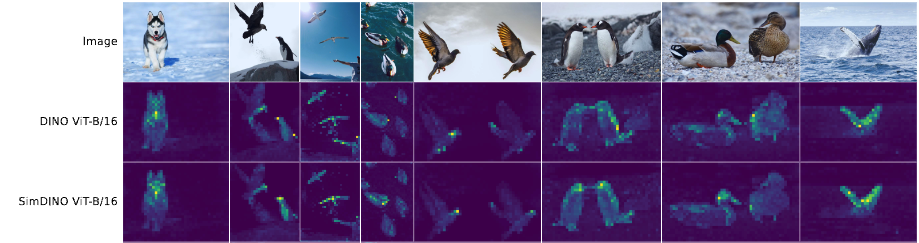
\includegraphics[width=\textwidth]{\toplevelprefix/chapters/chapter7/figs/dino_attention_maps.png}
    \caption{\small\textbf{O comparație calitativă a hărților de saliență} generate de DINO \textit{(rândul din mijloc)} și de SimDINO \textit{(rândul de jos)}. Pentru fiecare imagine, calculăm și afișăm harta de saliență medie în ultimul strat \(L\). Hărțile de saliență sunt similare între modele, ceea ce înseamnă că toate modelele converg la o noțiune similară despre ce obiecte sunt importante. Rețineți că, deși \(X_{\evaluation}\) este o imagine pătrată, este interpolată înapoi în formă dreptunghiulară pentru a face această vizualizare.}
    \label{fig:dino_attention_maps_saliency}
\end{figure}

\begin{table}
    \centering 
    \begin{tabular}{@{}llcccccccc@{}}
        \toprule
         &  & \multicolumn{3}{c}{Detecție $\uparrow$} &  \multicolumn{3}{c}{Segmentare $\uparrow$} \\ 
        Metodă & Model & AP$_{50}$  & AP$_{75}$ & AP & AP$_{50}$ & AP$_{75}$ & AP  \\ 
        \midrule
        SimDINO &ViT-L/16 &\bf 5.4 &1.9 &2.4 &4.5 &1.4 &1.9 \\
        SimDINO &ViT-B/16 &5.2 & \bf 2.0 & \bf 2.5 & \bf4.7 & \bf 1.5 & \bf 2.0 \\
        DINO &ViT-B/16 &3.9 &1.5 &1.8 &3.1 &1.0 &1.4 \\
        \midrule
        \color{gray} DINO & \color{gray} ViT-B/8 & \color{gray}5.1 & \color{gray}2.3 & \color{gray}2.5 & \color{gray}4.1 & \color{gray}1.3 & \color{gray}1.8 \\
        \bottomrule
    \end{tabular}
    \caption{\small\textbf{Performanța de segmentare} a modelelor DINO și SimDINO pre-antrenate pe COCO val2017 \citep{lin2014microsoft}, un set de date de segmentare care conține metadate de localizare a obiectelor. Nu antrenăm pe COCO, folosind doar încorporarea și coloana vertebrală pre-antrenate, iar casetele de delimitare sunt extrase din caracteristici printr-o metodă numită MaskCut \citep{wang2023cut}. Cu toate acestea, SimDINO depășește DINO la detecția și segmentarea obiectelor sub comparație corectă și chiar depășește DINO cu dimensiune mai mică a patch-ului (lungime laterală \(8\) în loc de \(16\)). Dimensiunile mai mici ale patch-urilor sunt cunoscute că ajută performanța, în special cu sarcinile de detecție și segmentare, așa că acest rezultat este destul de surprinzător și încurajator.}
    \label{tab:dino_segmentation}
\end{table}

\paragraph{Rezultatele evaluării.} În ceea ce privește performanța de clasificare în aval, obținem performanța din \Cref{tab:dino_imagenet_linear_probing}. Observăm că performanța SimDINO este mult mai mare decât cea a DINO sub comparație corectă. De asemenea, este mult mai stabilă: setările prescrise ale DINO nu pot antrena un model ViT-L(arge). Pe de altă parte, \Cref{fig:dino_attention_maps_saliency} arată vizualizări ale hărților de saliență medie în DINO și DINO-ul nostru simplificat, observând că hărțile de saliență arată destul de similar între modele, indicând că modelele învață caracteristici care sunt cel puțin la fel de bune la captarea detaliilor fine. Performanțele de segmentare și detecție a obiectelor din \Cref{tab:dino_segmentation} confirmă această afirmație cantitativ, unde caracteristicile SimDINO arată o îmbunătățire substanțială față de cele ale DINO.



\section{Clasificarea Imaginilor}\label{sec:image_classification}

În secțiunea anterioară, am simplificat un obiectiv de învățare excesiv de complex folosind intuiția noastră despre învățarea reprezentărilor prin prisma compresiei. Cu toate acestea, multe dintre cele mai populare proceduri de învățare sunt incredibil de simple. În aceste cazuri, este dificil să simplificăm și mai mult obiectivul. Astfel, în aceasta și în secțiunile viitoare, ne vom concentra pe modalități principiale de a modifica \textit{arhitecturile de rețele profunde} pentru o varietate de sarcini.

Să începem mai întâi cu, fără îndoială, cea mai clasică sarcină din învățarea automată: \textit{clasificarea imaginilor}, care este adesea folosită ca sarcină standard pentru a evalua algoritmii de recunoaștere a modelelor sau arhitecturile de rețele profunde. Din discuția noastră despre arhitecturi white-box din \Cref{ch:representation}, avem nevoie doar de o sarcină semnificativă semantic pentru a învăța reprezentări bune cu arhitecturi white-box. Vom valida această idee în această secțiune.

Mai întâi, setul de date rămâne în mare parte același ca în \Cref{sub:contrastive_learning_data}. Atât datele de antrenament, cât și cele de test constau din imagini etichetate, adică perechi imagine-etichetă \((\vX, \vy) \in \R^{C \times H \times W} \times \{0, 1\}^{N_{\cls}}\). Aplicăm în continuare diverse augmentări de date (de exemplu, răsturnări, blur Gaussian, solarizare etc.) la fiecare mostră din fiecare lot nou.

\subsection{Sarcină și Obiectiv} \label{sub:image_classification_objective}

Spre deosebire de înainte, sarcina noastră nu este doar să învățăm o reprezentare bună a datelor, ci și să construim simultan un clasificator. Formal, avem perechi de date etichetate \((\vX, \vy)\), unde \(\vy \in \{0, 1\}^{N_{\cls}}\) este un vector one-hot care denotă apartenența la clasă a lui \(\vX\). Considerăm o \textit{vedere de decupare centrală} deterministă \(v_{\cc}\) a datelor de intrare \(\vX\) (cf \Cref{sub:contrastive_learning_objective}). Vrem să antrenăm împreună o mapare de caracteristici \((f_{\theta}, f_{\theta}^{\ext})\) și un \textit{cap de clasificare} \(h_{\theta}\), definit după cum urmează:
\begin{equation}
    h_{\theta}(\vz) \doteq \softmax(\vW^{\head}\vz + \vb^{\head}), \qquad  \forall \vz \in \R^{d}
\end{equation}
unde \((\vW^{\head}, \vb^{\head}) \in \R^{N_{\cls} \times d} \times \R^{N_{\cls}}\) sunt parametri antrenabili în setul de parametri \(\theta\), astfel încât harta \(\vX_{\cc} \mapsto \vp_{\theta}(\vX_{\cc}) \doteq h_{\theta}(\vz_{\theta}(\vX_{\cc}))\) prezice o etichetă netedă pentru vederea \(\vX_{\cc} = v_{\cc}(\vX)\) a intrării \(\vX\). Problema de învățare încearcă să minimizeze distanța dintre \(\vp_{\theta}\) și \(\vy\) măsurată prin entropie încrucișată:
\begin{equation}\label{eq:classification_ce_loss}
    \min_{\theta}\bc{\cL_{\CE}(\theta) \doteq \Ex[\CE(\vy, \vp_{\theta}(\vX_{\cc}))]}.
\end{equation}


\subsection{Arhitectura CRATE}\label{sub:image_classification_architecture}

Arhitectura pe care o folosim este arhitectura CRATE, descrisă în detaliu în \Cref{ch:representation}. Configurarea generală este similară cu cea a transformerului obișnuit din \Cref{sub:contrastive_learning_architecture}, cu câteva modificări. În timp ce pasul de încorporare este același ca atât DINO, cât și SimDINO în \Cref{sub:contrastive_learning_architecture}, pasul de extracție a caracteristicilor este același ca SimDINO în \Cref{sub:contrastive_learning_architecture}, deoarece doar extrage caracteristica corespunzătoare token-ului de clasă, iar capul de clasificare este descris în \Cref{sub:image_classification_objective}, arhitectura coloanei vertebrale este diferită. Fiecare strat ia forma
\begin{align}\label{eq:CARTE updates}
    \vZ_{\theta}^{\ell + 1/2}(\vX)
    &= \vZ_{\theta}^{\ell}(\vX) + \MSSA_{\theta}^{\ell}(\LN_{\theta}^{1, \ell}(\vZ_{\theta}^{\ell}(\vX))), \\ 
    \vZ_{\theta}^{\ell + 1}(\vX)
    &= \ISTA_{\theta}^{\ell}(\LN_{\theta}^{2, \ell}(\vZ_{\theta}^{\ell + 1/2}(\vX))),
\end{align}
unde blocurile \(\MSSA_{\theta}^{\ell}\) și \(\ISTA_{\theta}^{\ell}\) sunt așa cum sunt descrise în \Cref{ch:representation}, anume:
\begin{itemize}
    \item Operatorul \(\MSSA\) este auto-atenție multi-cap-subspațiu, definit după cum urmează:
    \begin{equation}
        \MSSA_{\theta}^{\ell}(\vZ) \doteq \vU_{\out}^{\ell}\mat{\SA([\vU^{1, \ell}]^{\top}\vZ, [\vU^{1, \ell}]^{\top}\vZ, [\vU^{1, \ell}]^{\top}\vZ)\\ \vdots \\ \SA([\vU^{K, \ell}]^{\top}\vZ, [\vU^{K, \ell}]^{\top}\vZ, [\vU^{1, \ell}]^{\top}\vZ)} + \vb_{\out}^{\ell}\vone_{n}^{\top}
    \end{equation}
    unde \(\vU^{k, \ell} \in \R^{d \times p}\), \(\vU_{\out}^{\ell} \in \R^{d \times Kp}\), și \(\vb_{\out}^{\ell} \in \R^{d}\) sunt parametri antrenabili aparținând setului de parametri \(\theta\), și (amintiți-vă) operatorul de auto-atenție \(\SA\) este definit în \eqref{eq:self_attention}.
    \item Operatorul \(\ISTA\) este operatorul algoritm-iterativ-de-micșorare-pragare, definit după cum urmează:
    \begin{equation}
        \ISTA_{\theta}^{\ell}(\vZ) \doteq \ReLU(\vZ - \beta (\vD^{\ell})^{\top}(\vD^{\ell}\vZ - \vZ) + \beta\lambda \vone_{d}\vone_{n}^{\top}),
    \end{equation}
    numit astfel deoarece harta \(\vX \mapsto \ReLU(\vX - \beta \vD^{\top}(\vD\vX - \vZ) + \beta  \lambda \vone_{d}\vone_{n}^{\top})\) este un pas al algoritmului ISTA bine stabilit pentru a găsi o reprezentare rară non-negativă element cu element pentru \(\vZ\) în raport cu dicționarul complet \(\vD\) (cf \Cref{sec:dictionary_learning}).
\end{itemize}

Numim această arhitectură CRATE, iar un strat al coloanei vertebrale este ilustrat în \Cref{fig:crate_backbone}. Modelele CRATE, pe lângă faptul că sunt interpretabile, sunt în general și foarte performante și eficiente din punct de vedere al parametrilor.

\subsection{Optimizare} \label{sub:image_classification_optimization}

Antrenăm clasificatorul nostru folosind o procedură simplă de optimizare stocastică end-to-end, unde sub-eșantionăm date și vederi, calculăm pierderea medie și gradientul său peste aceste mostre și folosim un algoritm de optimizare pentru a schimba parametrii. La fiecare pas de timp \(k\):
\begin{itemize}
    \item Sub-eșantionăm \(B\) mostre etichetate diferite \(\{(\vX_{b}^{(k)}, \vy_{b}^{(k)})\}_{b = 1}^{B} \subseteq \cI \times \{0, 1\}^{N_{\cls}}\).
    \item Pentru fiecare mostră etichetată \((\vX_{b}^{(k)}, \vy_{b}^{(k)})\), calculăm vederea de decupare centrală \(v_{b, \cc}^{(k)}\) și o aplicăm la \(\vX_{b}^{(k)}\) pentru a obține \(\vX_{b, \cc}^{(k)} \doteq v_{b, \cc}^{(k)}(\vX_{b}^{(k)})\).
    \item Calculăm predicțiile \(\vp_{\theta}(\vX_{b, \cc}^{(k)}) \doteq (h_{\theta} \circ f_{\theta}^{\ext} \circ f_{\theta})(\vX_{b, \cc}^{(k)})\).
    \item Formăm pierderea stocastică surogat 
    \begin{equation}
        \hat{\cL}_{\CE}^{(k)}(\theta) \doteq \frac{1}{B}\sum_{b = 1}^{B}\CE(\vy_{b}^{(k)}, \vp_{\theta}(\vX_{b, \cc}^{(k)})).
    \end{equation}
    \item Calculăm un pas al unui algoritm de optimizare pe \(\theta\), dând următoarea iterație:
    \begin{equation}
        \theta^{(k + 1)} \doteq \textsc{OptUpdate}^{(k)}(\theta^{(k)}; \nabla_{\theta}\hat{\cL}_{\CE}^{(k)}).
    \end{equation}
\end{itemize}


\subsection{Metodologie de Evaluare} \label{sub:image_classification_evals}

Folosim aceeași procedură de evaluare ca în \Cref{sub:contrastive_learning_evals}. Pentru a rezuma, pentru toate evaluările (precum și antrenamentul) folosim o vedere de decupare centrală \(v_{\cc}\) care redimensionează imaginea de intrare și ia o decupare centrală mare de dimensiune \((C, S_{\cc}, S_{\cc})\) unde \(C\) este numărul de canale din imaginea de intrare. Putem apoi face sondare liniară, vizualizare a hărților de atenție și benchmark-uri de detecție/segmentare, date ieșirea acestei vederi.

\subsection{Configurare Experimentală și Rezultate}\label{sub:image_classification_experiments}

Deoarece CRATE este bazat direct pe transformer, comparăm setările optime pentru ViT așa cum sunt date de \cite{dosovitskiy2020image,touvron2020training} cu aceleași setări aplicate la CRATE pentru o comparație corectă.

\paragraph{Arhitectura modelului.} Decuparea centrală redimensionează întreaga imagine astfel încât marginea mai scurtă să fie de dimensiune \(256\) (adică, \(S_{\rsz} = 256\)) înainte de a lua o decupare centrală de dimensiune \(224 \times 224\) (adică, \(S_{\cc} = 224\)), atât în evaluare, cât și în antrenament. Luăm dimensiunea patch-ului \(16\) (adică, \(P_{H} = P_{W} = 16\)). Folosim modelele mici, de bază și mari ale arhitecturii ViT \cite{dosovitskiy2020image} ca încorporare și coloană vertebrală, înlocuind componentele MHSA și MLP cu MSSA și ISTA, respectiv, folosind același număr de capete și dimensiune a capului în cazul MSSA, și prin urmare reducând drastic numărul de parametri de antrenament. Pentru CRATE, setăm \((\beta, \lambda) = (1, 0.1)\).

\paragraph{Seturi de date și optimizare.} Pentru pre-antrenament, folosim setul de date ImageNet-1K. Folosim optimizatorul LION \citep{chen2024symbolic} pentru a pre-antrena atât replicarea noastră ViT, cât și CRATE. Setăm rata de învățare de bază ca \(2.4 \times 10^{-4}\), decăderea ponderilor ca \(0.5\) și dimensiunea lotului ca \(B = 2048\). Programul nostru de rată de învățare crește rata de învățare liniar la rata de învățare de bază în primele \(5\) epoci și scade la \(0\) folosind un program cosinus în următoarele \(145\) epoci (antrenând toate modelele pentru \(150\) epoci fiecare). Pentru pre-antrenament, aplicăm un regim obișnuit de augmentări de date (răsturnări, blur-uri Gaussiene, solarizare etc.) la datele de imagine și adăugăm și zgomot mic la etichete (aceasta se numește \textit{netezirea etichetelor} \citep{muller2019does}).

Pentru sondarea liniară, folosim mai multe seturi de date de evaluare, cum ar fi CIFAR10, Oxford-Flowers și Oxford-IIT-Pets. Folosim optimizatorul AdamW pentru a antrena sonda liniară, folosind rata de învățare \(5 \times 10^{-5}\), decăderea ponderilor \(0.01\) și dimensiunea lotului \(B = 256\). Aplicăm de asemenea augmentările de date menționate anterior la datele de imagine.

\begin{table}
    \centering
    \begin{tabular}{@{}lcccc|cc@{}}
    \toprule
    \textbf{Model} & CRATE-T  &  CRATE-S & CRATE-B & CRATE-L & { \color{gray} ViT-T} &  { \color{gray}ViT-S } \\ 
    \midrule
    \midrule
     \# parametri & 6.09M & 13.12M & 22.80M & 77.64M & { \color{gray} 5.72M} & { \color{gray} 22.05M} \\
    \midrule
     ImageNet-1K & 66.7 & 69.2 & 70.8 & 71.3 & { \color{gray} 71.5} & { \color{gray} 72.4} \\
     ImageNet-1K ReaL & 74.0 & 76.0 & 76.5 & 77.4 & { \color{gray} 78.3 } & { \color{gray} 78.4} \\
     CIFAR10 & 95.5 & 96.0 & 96.8 & 97.2 & { \color{gray} 96.6} & { \color{gray} 97.2} \\
     CIFAR100 & 78.9 & 81.0 & 82.7 & 83.6 & { \color{gray} 81.8} & { \color{gray} 83.2}\\
     Oxford Flowers-102 & 84.6 & 87.1 & 88.7 & 88.3 & { \color{gray} 85.1} & { \color{gray} 88.5}\\
     Oxford-IIIT-Pets & 81.4 & 84.9 & 85.3 & 87.4 & { \color{gray} 88.5} & { \color{gray} 88.6} \\
     \bottomrule
    \end{tabular}
    \caption{\small \textbf{Acuratețea clasificării prin sondare liniară a CRATE și ViT} pe diverse seturi de date cu diferite dimensiuni de model când coloana vertebrală este pre-antrenată pentru clasificare pe ImageNet-1K. Observăm că, dată fiind aceeași configurație de model, CRATE are performanță de clasificare comparabilă cu un design mai simplu, mai principial și mai eficient din punct de vedere al parametrilor.}
    \label{tab:crate_classification_linear_probing}
\end{table}

\begin{figure}[t]
    \centering
    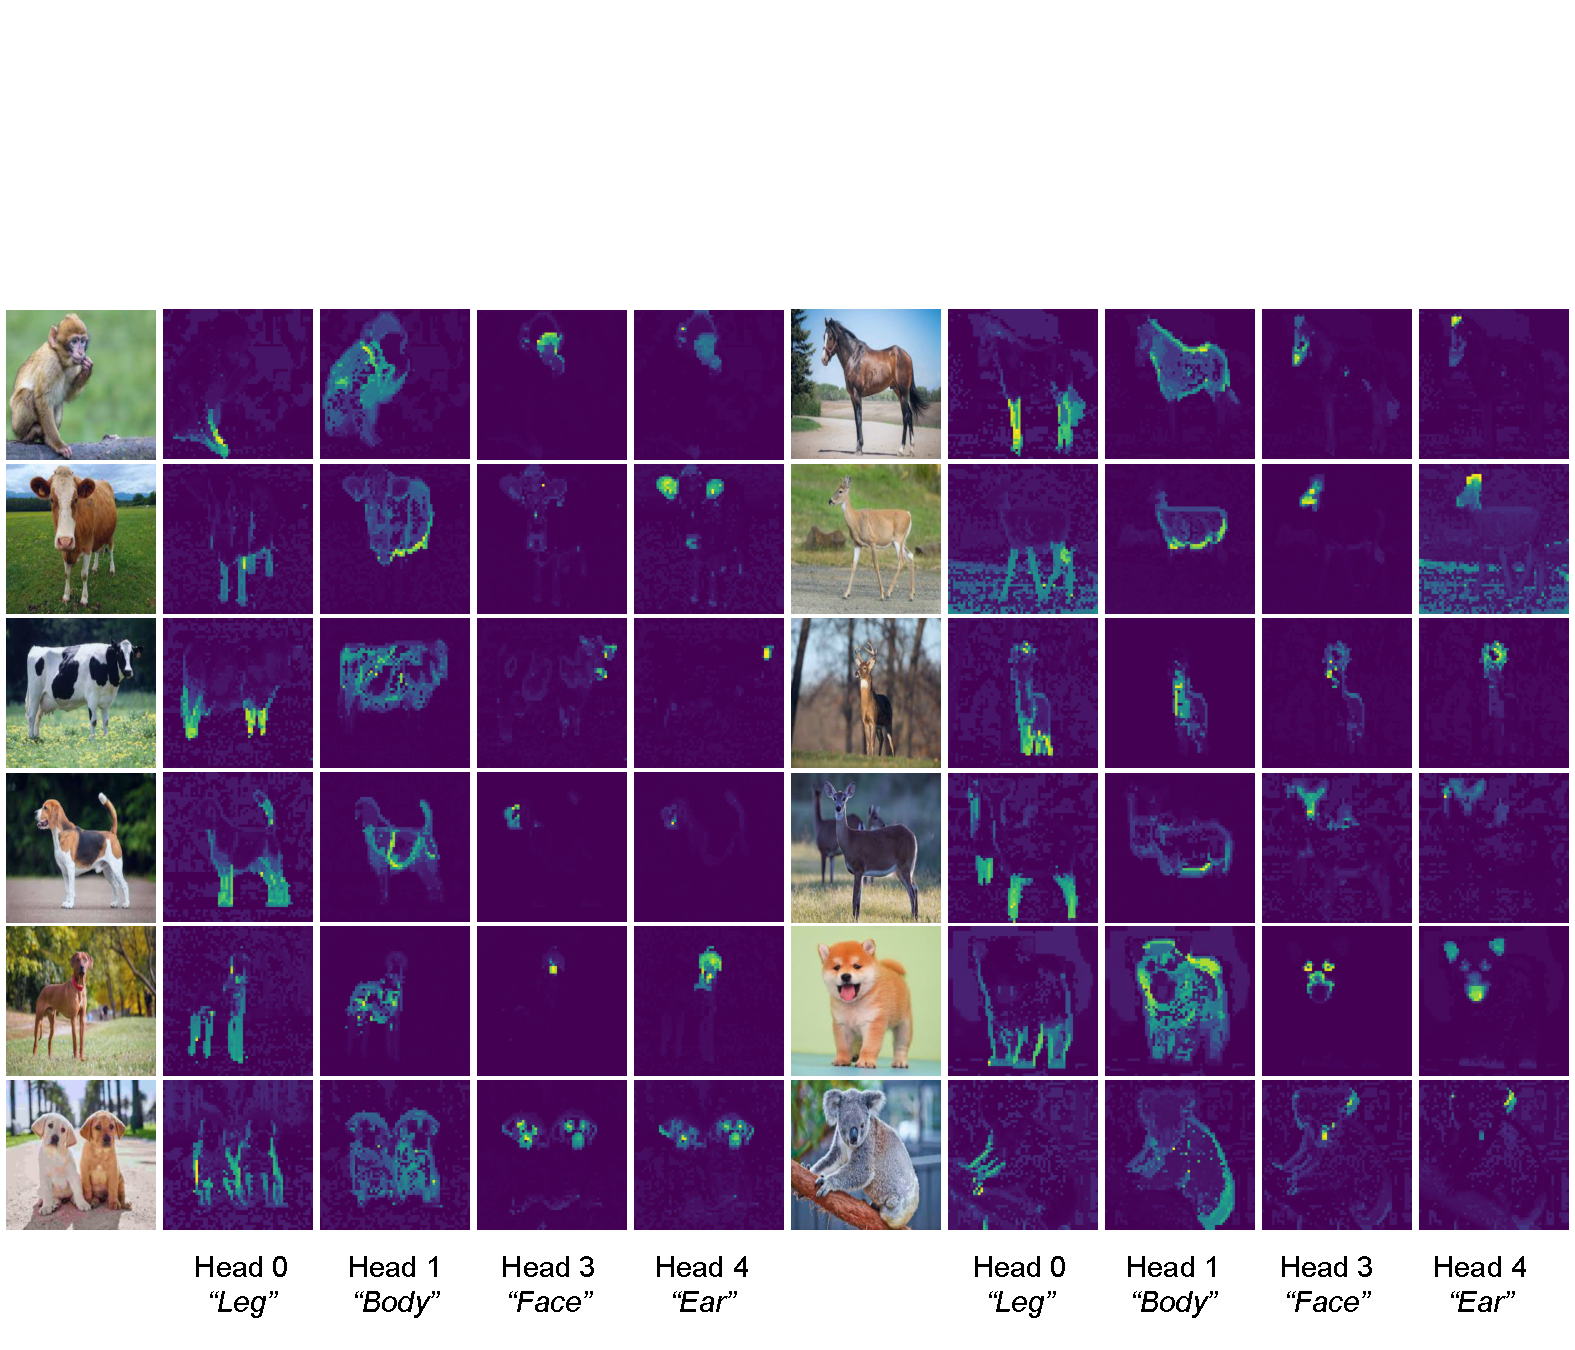
\includegraphics[width=0.8\textwidth]{\toplevelprefix/chapters/chapter7/figs/crate_semantic_heads.pdf}
    \caption{\small\textbf{Hărți de saliență interpretabile în CRATE} cu dimensiunea patch-ului \(8\). Când sunt date imagini cu proprietăți similare (poate dar nu neapărat din aceeași clasă), hărțile de saliență corespunzătoare diferitelor capete de atenție din ultimul strat evidențiază fiecare o proprietate specifică. Se poate observa că harta de saliență medie (neinclusă) evidențiază apoi toate obiectele relevante din imagine, arătând că folosește toate detaliile fine ale imaginii de intrare pentru clasificare. Acesta este \textit{primul} sistem de învățare automată care face acest lucru, după cunoștințele autorilor, cu atât mai puțin automat fără antrenament pe date de segmentare.}
    \label{fig:crate_semantic_heads}
\end{figure}

\begin{table}
    \centering
    \begin{tabular}{@{}lcccccccc@{}}
    \toprule
     &  \multicolumn{3}{c}{Detecție (\(\uparrow\))} &  \multicolumn{3}{c}{Segmentare (\(\uparrow\))} \\ 
    Model & AP$_{50}$ & AP$_{75}$ & AP & AP$_{50}$ & AP$_{75}$ & AP  \\ 
    \midrule
    CRATE-S/8 & \textbf{2.9} & \textbf{1.0} & 1.1 & 1.8 & \textbf{0.7} & 0.8 \\
    CRATE-B/8 & \textbf{2.9} & \textbf{1.0} & \textbf{1.3} & \textbf{2.2} & \textbf{0.7} & \textbf{1.0} \\
    ViT-S/8 & 0.1& 0.1 & 0.0 & 0.0 & 0.0 & 0.0 \\
    ViT-B/8 & 0.8 & 0.2 & 0.4 & 0.7 & 0.5 & 0.4 \\
    \bottomrule
    \end{tabular}
    \caption{\small \textbf{Detecția obiectelor și segmentarea fină prin MaskCut pe COCO {val2017}~\citep{lin2014microsoft}}. Aici toate modelele sunt antrenate cu dimensiunea patch-ului \(8\) în loc de \(16\). CRATE performează concludent mai bine decât ViT la metricile de detecție și segmentare când ambele sunt antrenate folosind clasificare supervizată.}
    \label{tab:crate_detection_segmentation}
\end{table}


\paragraph{Rezultate experimentale.} 

\Cref{tab:crate_classification_linear_probing} demonstrează că modelele CRATE ating paritate sau îmbunătățire comparativ cu populara arhitectură Vision Transformer (ViT) la numere similare de parametri, cel puțin în termeni de separabilitate liniară a caracteristicilor lor în raport cu diferite clase. În ceea ce privește fidelitatea hărților de atenție, \Cref{fig:crate_semantic_heads} demonstrează un rezultat cu adevărat extraordinar: fără a fi nevoie să se antreneze pe date de segmentare sau detecție a obiectelor, \textit{nu doar} că hărțile de saliență captează eficient toate părțile relevante ale imaginii de intrare, hărțile de saliență \textit{se auto-organizează} pentru a corespunde fiecare unui set discret de concepte, chiar și între mostre și clase! Acesta este primul sistem care face acest lucru, după cunoștințele autorilor, și poate face acest lucru fără a folosi date suplimentare, cu excepția datelor de clasificare a imaginilor. \Cref{tab:crate_detection_segmentation} confirmă aceste perspective calitative cantitativ, arătând o îmbunătățire semnificativă față de ViT-urile antrenate în aceeași configurație de clasificare supervizată.

\section{Modelarea Limbajului Cauzal}\label{sec:clm_text}

Studiem acum \textit{modelarea limbajului cauzal}, o metodă pentru antrenarea modelelor mari de limbaj (LLM). Aceasta este aceeași configurare folosită pentru a antrena, printre multe altele, GPT-2 și multe alte modele de limbaj.

\subsection{Date} \label{sub:clm_text_data}

Datele pe care le vom folosi pentru a investiga performanța CRATE pentru sarcini de limbaj vor fi OpenWebText (OWT)~\cite{Gokaslan2019OpenWeb}, o reproducere open-source a setului de date WebText nedivulgat folosit de OpenAI pentru a antrena GPT2. Fiecare mostră din OWT este un document web, de obicei provenit din pagini web de înaltă calitate, bloguri, articole sau discuții online, care este scris în limbaj natural bine format. Setul de date OpenWebText conține aproximativ 8.01M documente de lungimi variate, totalizând aproximativ 41.70GB de text. Pentru evaluare, vom folosi mai multe seturi de date, cum ar fi WikiText~\cite{merity2016pointer}\footnote{Pentru WikiText2 și WikiText103~\cite{merity2016pointer}, împărțirile de test sunt aceleași, așa că le îmbinăm ca un singur set de date denumit WikiText.}, LAMBADA~\cite{paperno2016lambadadatasetwordprediction}\footnote{Pentru a obține acuratețea pe setul de date LAMBADA, folosim decodare lacomă.} și PTB~\cite{marcus-etal-1993-building}. PTB și OWT sunt în general mai ușoare comparativ cu alte seturi de date. PTB se concentrează pe text jurnalistic mai simplu, ideal pentru modelarea tradițională a limbajului, în timp ce OWT este divers și informal, acoperind diverse subiecte, dar cu mai puțină complexitate în structura limbajului sau dependențe pe termen lung. WikiText, cu structura sa formală și conținutul specific domeniului, necesită o înțelegere mai complexă decât OWT, dar rămâne gestionabil. LAMBADA este cel mai provocator, deoarece implică dependențe pe termen lung, necesitând ca modelul să înțeleagă informații contextuale mai largi pentru a completa propozițiile cu acuratețe.

La un nivel mai formal, datele noastre \(\vX\) vor fi text sau șiruri de caractere; lăsăm \(\cT\) să fie setul tuturor șirurilor.

\subsection{Sarcină și Obiectiv} \label{sub:clm_text_objective}

Pentru pre-antrenamentul modelării limbajului cauzal, ideea este că vrem să \textit{antrenăm modelul să producă text asemănător cu cel uman}. Cea mai populară modalitate de a face acest lucru este să folosim un proces de antrenament în două etape:\footnote{Antrenamentul modern al modelelor de limbaj are mai multe etape suplimentare de antrenament care necesită distribuții de date diferite și abordări algoritmice diferite. Cu toate acestea, antrenarea unui model pentru a imita doar scrierea umană necesită doar acești câțiva pași prezentați.}
\begin{itemize}
    \item \textit{Mai întâi}, dorim să \textit{învățăm} o modalitate de a codifica optim documentele ca o secvență de șiruri de bază („blocuri de construcție"), numite \textit{token-uri}. Aceasta se numește \textit{tokenizare}, și construim un \textit{tokenizator}.
    \item \textit{În al doilea rând}, dorim să \textit{învățăm} o modalitate de a \textit{prezice distribuția unui token dat toate token-urile anterioare}. Aceasta se numește \textit{predicție de următorul token}, și construim un \textit{model de limbaj}.
\end{itemize}
Această procedură datează de fapt de la Markov, care a observat pentru prima dată că limbajul natural ar putea fi modelat prin structura de lanț Markov eponimă \citep{markov2006example} dată o tokenizare adecvată, și apoi la Shannon, care a propus să facă exact această configurare de modelare a limbajului cu un tokenizator la nivel de caracter (adică, fiecare caracter este un token) și așa-numitele „\(n\)-grame" (adică, o tabelă de căutare explicită, calculată din datele de antrenament, pentru distribuția unui token dat cele \(n\) token-uri anterioare) în locul modelului de limbaj \citep{Shannon-1948}.\footnote{Un studiu recent \citep{liu2024infini} care scalează modelele \(n\)-gram a arătat că sunt capabile să modeleze textul rezonabil de bine pentru \(n\) mare, dar bineînțeles memoria necesară pentru a stoca o astfel de tabelă de căutare este de ordinul \(V^{n}\) și prin urmare complet intractabilă.}

\subsubsection{Antrenarea unui Tokenizator}

Pentru a construi un tokenizator înseamnă să construim un vocabular \(\cV\), care este un set de token-uri și are o dimensiune pre-specificată \(V\). Există mai multe metode pentru a face acest lucru. Un algoritm popular este cunoscut sub numele de Codare Pereche de Octeți (BPE), care poate fi descris ca:
\begin{itemize}
    \item Începem cu o listă a tuturor caracterelor unice din datele de antrenament și frecvențele lor. Asigurăm-ne că există mai puțin de \(V\) astfel de caractere și adăugăm fiecare caracter ca un șir separat („token") la vocabular împreună cu frecvența sa.
    \item Până când există \(V\) token-uri în vocabular:
    \begin{itemize}
        \item Construim un token luând cele două token-uri existente cele mai frecvente și îmbinându-le.
        \item Calculăm frecvența acestui token în setul de date.
        \item Îl adăugăm la vocabular (împreună cu frecvența sa).
    \end{itemize} 
    \item În acest punct, informațiile de frecvență nu mai sunt necesare și pot fi eliminate.
\end{itemize}
Procesul general al BPE este în \Cref{fig:BPE}. Rețineți că această procedură este o modificare a unei proceduri clasice de compresie teoretico-informațională pentru \textit{învățarea unei codări fără pierderi} a datelor de flux de octeți (cum ar fi textul), și ca atare, se poate interpreta ca găsirea unei compresii optime fără pierderi a datelor. Observați că acest lucru este posibil deoarece (spre deosebire de imagini), datele aici sunt fundamental discrete și fără zgomot.
\begin{figure}
    \centering
    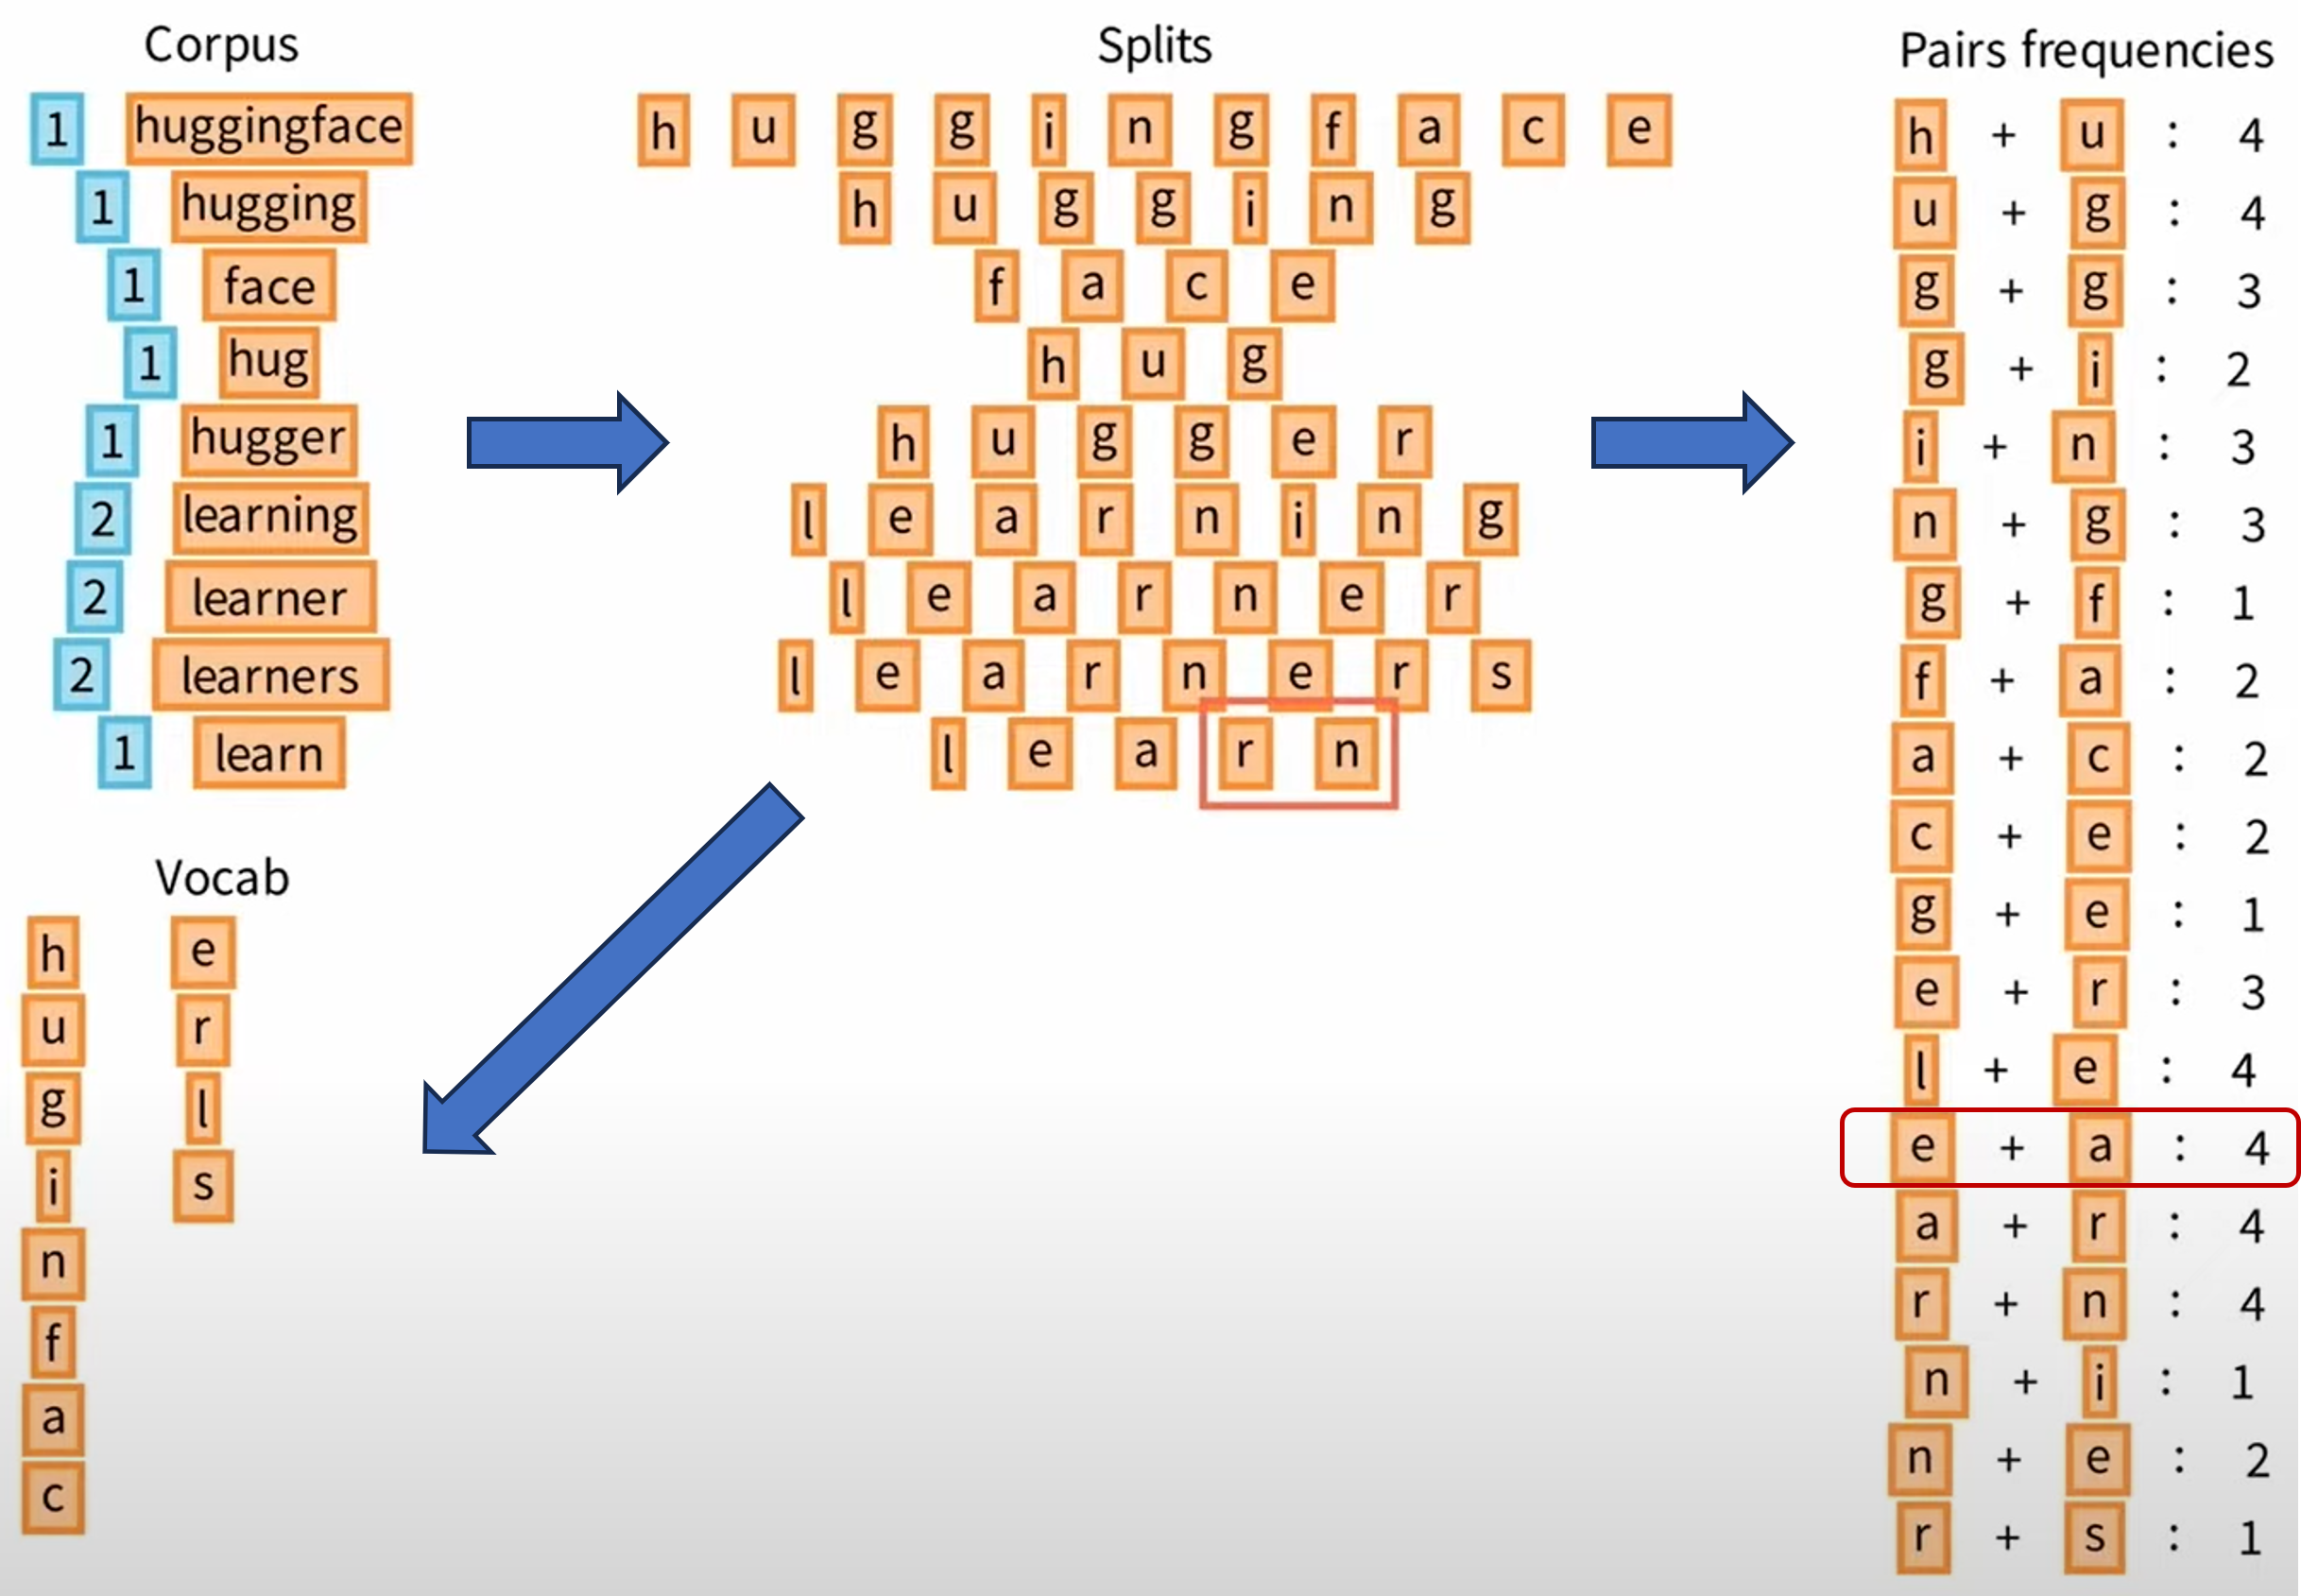
\includegraphics[width=0.45\textwidth]{\toplevelprefix/chapters/chapter7/figs/BPE1.png}\hspace{0.6in} 
    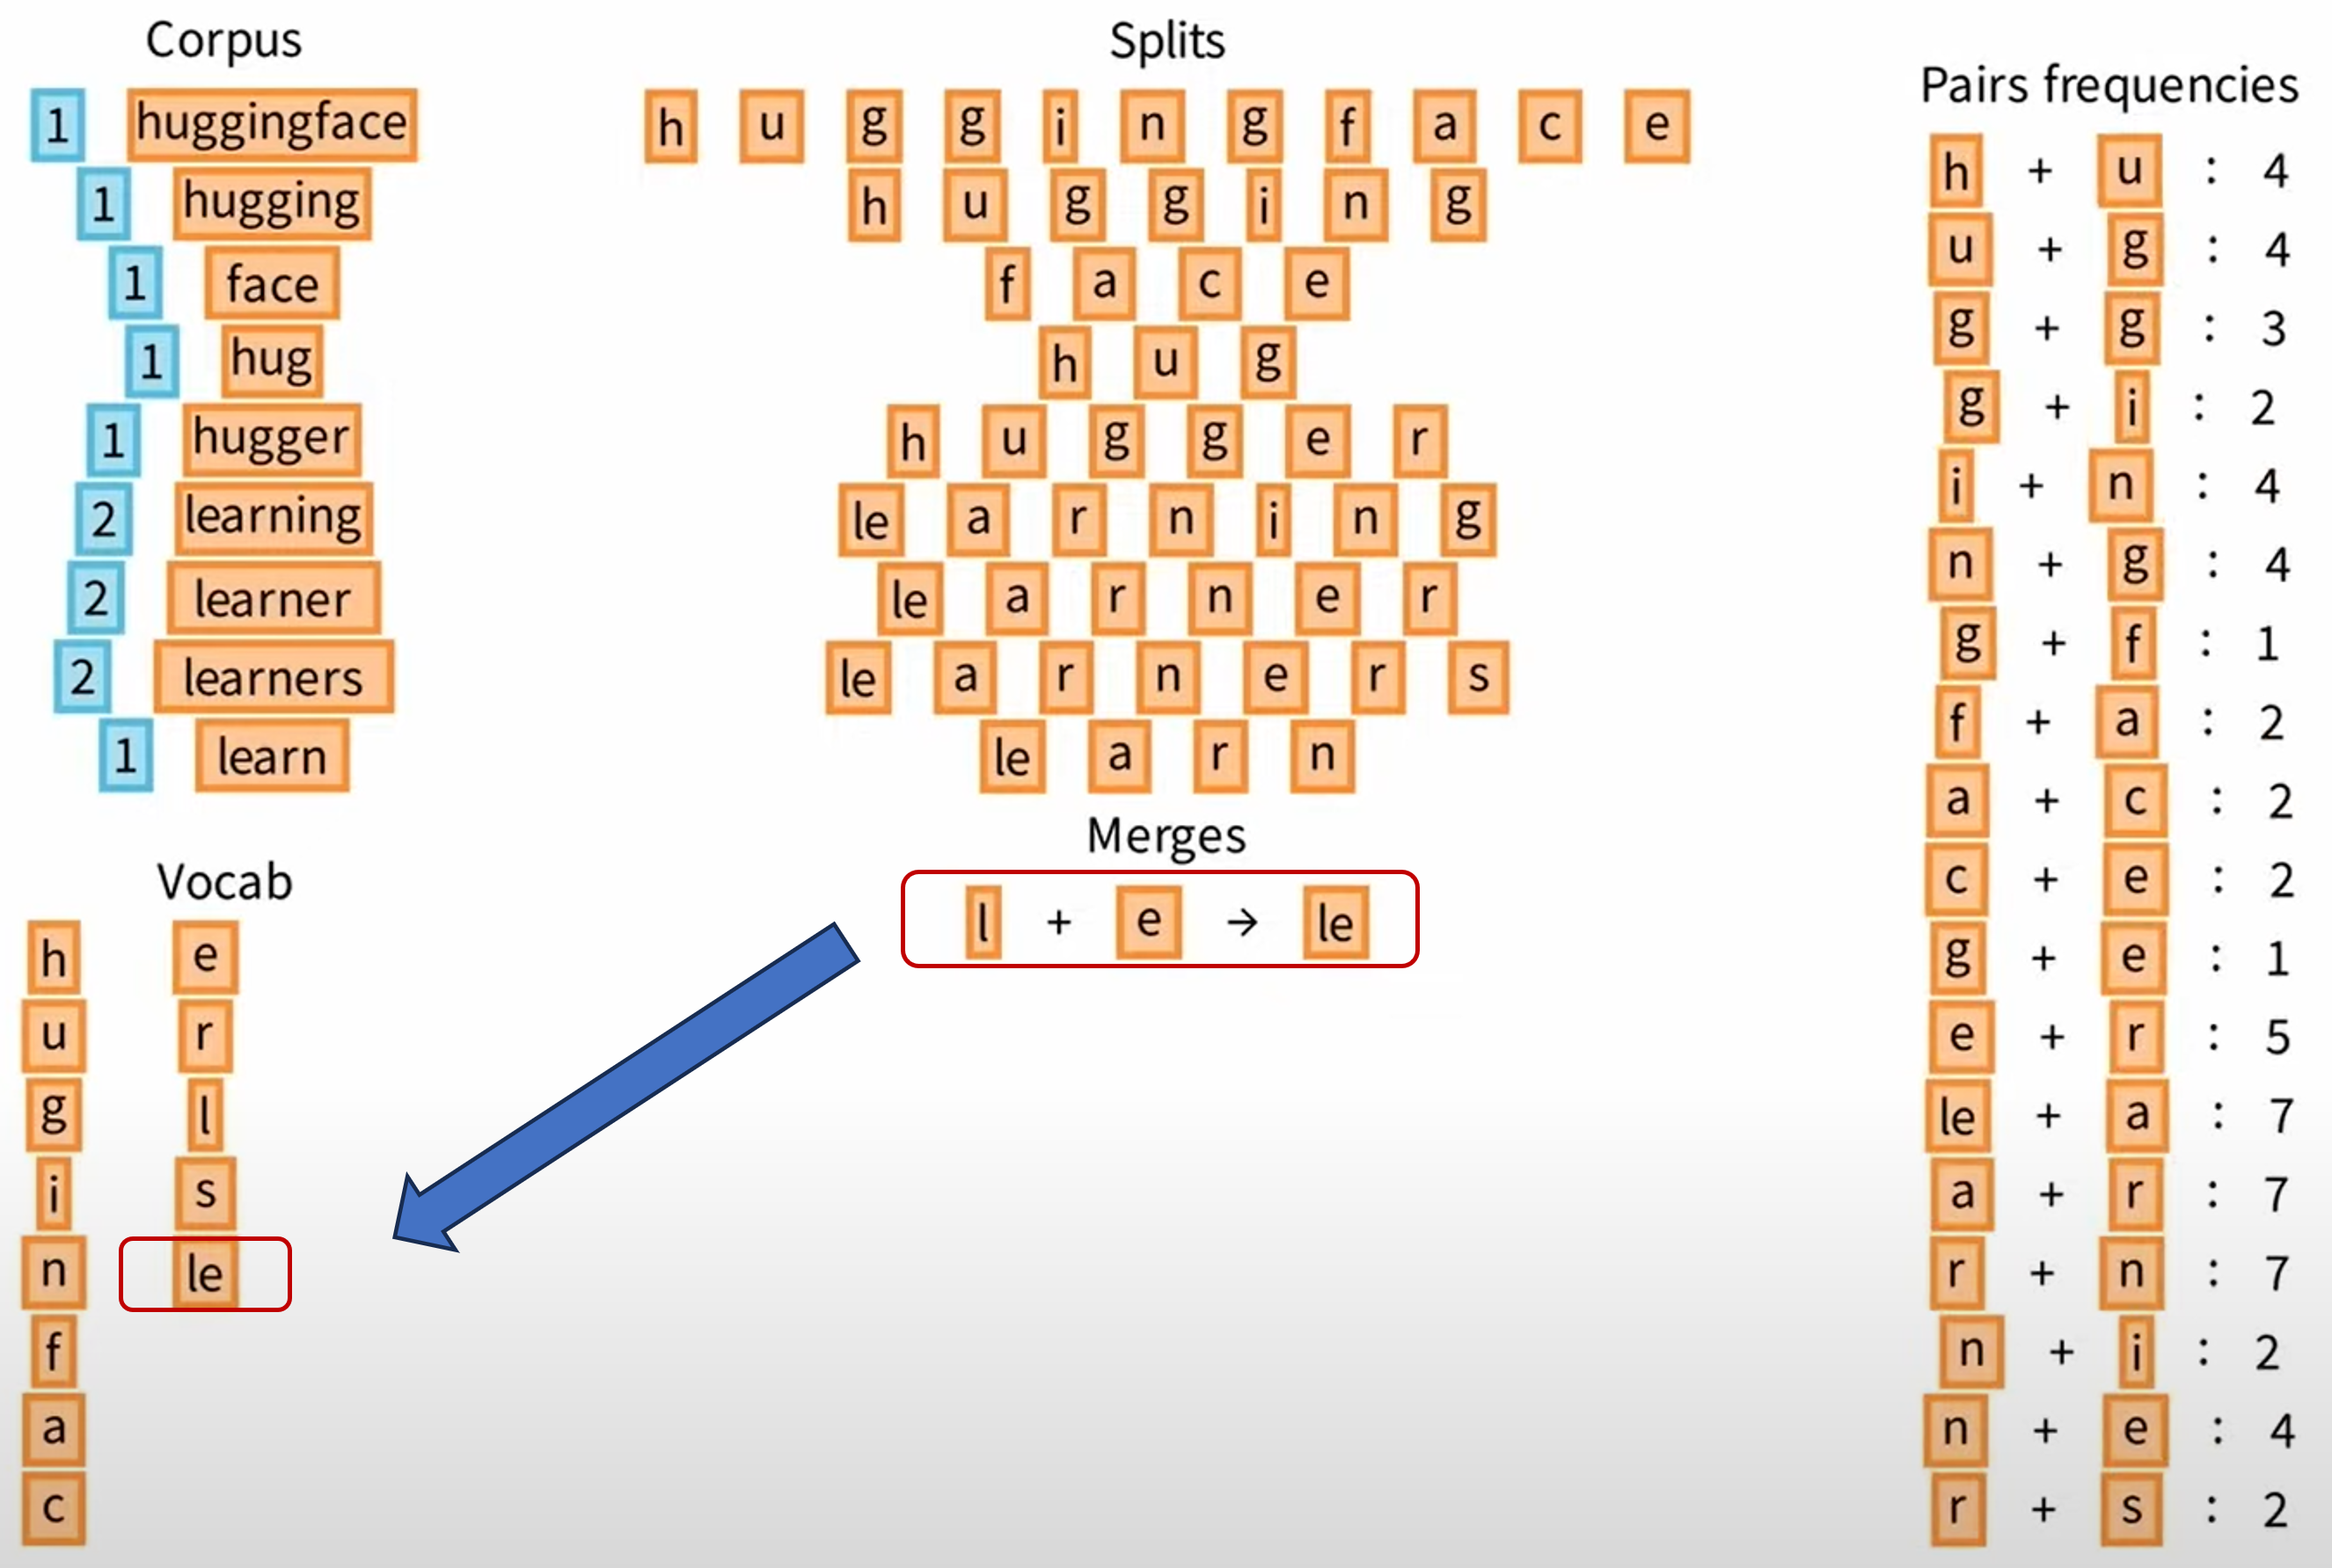
\includegraphics[width=0.45\textwidth]{\toplevelprefix/chapters/chapter7/figs/BPE2.png} 
    \caption{\small {\bf Procesul de tokenizare a datelor text folosind BPE.} (Credit imagine la \url{https://huggingface.co/learn/nlp-course/chapter6/5}). (Stânga) Începem prin analizarea corpusului de text dat și construirea unui vocabular inițial care constă din caractere individuale (sau octeți în cazul BPE la nivel de octet). Apoi, calculăm frecvențele perechilor de caractere adiacente în corpus. Aceasta implică scanarea întregului text și numărarea de câte ori apare fiecare secvență de două caractere (bigramă). (Dreapta) După calcularea frecvențelor perechilor de caractere adiacente, identificăm perechea cea mai frecventă în corpus. Această pereche este apoi îmbinată într-o nouă unitate de subcuvânt, care este adăugată la vocabular ca un singur token. Acest proces este repetat iterativ până când se atinge dimensiunea vocabularului predefinită.}
    \label{fig:BPE}
\end{figure}
După ce un astfel de vocabular este construit, un tokenizator poate descompune un document în token-uri (adică, să îl „tokenizeze"). BPE folosește o procedură similară pentru a tokeniza datele ca în antrenament:
\begin{itemize}
    \item Separăm documentul într-o listă lungă de token-uri de un caracter. Adică, dacă documentul este „Hello", atunci lista inițială este `H', `e', `l', `l', `o'. 
    \item În timp ce oricare două token-uri adiacente pot fi concatenate și concatenarea lor este un alt token, o facem, adică înlocuim această pereche de token-uri cu token-ul îmbinat. Anume, dacă `He' este un token în vocabular, `H', `e', `l', `l', `o' ar deveni `He', `l', `l', `o'.
    \item Repetăm procesul de mai sus până când nu se mai pot face îmbinări. În acest punct, documentul este partiționat în lista finală (secvența) de token-uri.
\end{itemize}

Există multe considerații practice și bazate pe eficiență de luat în considerare în timpul tokenizării. Algoritmul de mai sus, așa cum este prezentat, este \textit{foarte departe de a fi optim} dacă este implementat naiv, de exemplu. Nu acoperim acest subiect în detaliu mare; există multe resurse online pentru a învăța mai mult, cum ar fi \href{https://huggingface.co/learn/nlp-course/en/chapter6/5}{tutorialele HuggingFace}.

De exemplu, fiecare token are un \textit{index} corespunzător care este doar indexul său în vocabular (care, la urma urmei, este doar o listă de lungime \(V\)). Astfel, ieșirea majorității tokenizatoarelor este o listă de indici, să zicem un element al \([V]^{*}\). Țineți minte că acestea corespund sub-șirurilor documentului original, așa cum s-a arătat mai sus.

Odată ce un tokenizator este învățat, poate fi folosit ca o cutie neagră de orice model de limbaj. De exemplu, multe modele au același tokenizator (bazat pe OpenAI) bazat pe biblioteca \texttt{tiktoken}. În restul acestei secțiuni, vom folosi un astfel de tokenizator fix și pre-construit pentru totul și astfel identificăm fiecare document text \(\vX \in \cT\) cu versiunea sa tokenizată în \([V]^{*}\). Prin urmare, am putea la fel de bine să considerăm spațiul text \(\cT\) ca \textit{egal} cu spațiul secvențelor de token-uri \([V]^{*}\) (și nu pierdem nimic esențial).

\subsubsection{Antrenarea unui Model de Limbaj}

Odată ce avem fiecare document ca o secvență de token-uri \(\vX \in [V]^{N} \subseteq [V]^{*} = \cT\), dorim să efectuăm predicția următorului token. Adică, dat un \textit{context} \(\vX_{:n} \in [V]^{n}\) (adică, primele \(n\) token-uri \(\vx_{1}, \dots, \vx_{n} \in [V]\) din document)\footnote{Rețineți incongruența cu notația Python: aici notația \textit{include} indexul \(n\).}, dorim să prezicem token-ul \(\vx_{n + 1} \in [V]\) la poziția \(n + 1\). Pentru a face acest lucru, calculăm caracteristica agregată a lui \(\vX_{:n}\) prin \(\vz_{\theta}(\vX_{:n}) \doteq (f_{\theta}^{\ext} \circ f_{\theta})(\vX_{:n}) \in \R^{d}\), și folosim un cap de clasificare \(h_{\theta} \colon \R^{d} \to \Delta_{V}\) (implementat ca un strat liniar, MLP sau ceva puțin mai complicat) pentru a proiecta această caracteristică în simplexul de probabilitate \(V\)-dimensional \(\Delta_{V}\). Această proiecție \(\vp_{\theta}(\vX_{:n}) \doteq h_{\theta}(\vz_{\theta}(\vX_{:n}))\) servește ca o distribuție de probabilitate estimată a următorului token. Apoi, folosind notația \(\vone(\vx_{n + 1}) \in \Delta_{V}\) pentru a fi \(1\) în componenta \(\vx_{n + 1}\) și \(0\) în altă parte, pierderea de modelare a limbajului cauzal este
\begin{equation}\label{eq:clm_loss}
    \min_{\theta}\bc{\cL_{\mathrm{CLM}}(\theta) \doteq \Ex_{\vX}\rs{\frac{1}{N - 1}\sum_{n = 1}^{N - 1}\CE(\vone(\vx_{n + 1}), \vp_{\theta}(\vX_{:n}))}}
\end{equation}
Observați cât de similară este aceasta cu o pierdere de clasificare (să zicem pentru imagini); se folosește entropia încrucișată și se încearcă alinierea unui vector de probabilitate prezis cu adevărul de bază. Diferența majoră între aceste două pierderi este că în aceasta, calculăm pierderea pe o întreagă secvență, unde fiecare predicție este corelată cu celelalte (spre deosebire de cazul de clasificare i.i.d.).

Optimizarea acestei pierderi este de obicei numită „pre-antrenament" în comunitatea modelelor de limbaj (în contrast cu „post-antrenament" și, mai recent, „mid-antrenament", care sunt metodologii pentru a modifica un predictor de următorul-token pentru sarcini utile).

\textit{Notă marginală:} De ce primul termen din \eqref{eq:clm_loss} prezice \(\vone(\vx_{2})\), și nu există niciun termen care măsoară pierderea pentru a prezice primul token? Este pentru că dacă am dori să prezicem primul token, am avea \textit{secvența goală} ca context și, prin urmare, am face această primă predicție de token folosind un mecanism calitativ diferit de cel care se aplică celorlalte token-uri. Deci, de fapt, acest model nu este antrenat să prezică \textit{primul} token al oricărui document. Motivul pentru care acest lucru este OK se datorează unui detaliu de implementare al tokenizatorului: adesea, după construirea tokenizatorului, inserăm un token \textit{special} în vocabularul său, numit token-ul \textit{început-de-șir (sau document)} și etichetat \texttt{<|bos|>}.\footnote{Există de obicei mai multe token-uri speciale pentru scopuri diferite. Textul existent care conține token-urile speciale este procesat special.} Apoi, în timp ce procesăm fiecare document, adăugăm token-ul \texttt{<|bos|>} la începutul secvenței de token-uri a documentului, crescând lungimea secvenței tokenizate cu \(1\). Astfel, obiectivul de modelare a limbajului cauzal de mai sus are un termen care implică încercarea de a prezice primul token al documentului dat doar token-ul \texttt{<|bos|>} ca context, și astfel este o pierdere corectă conceptual.

\subsection{Arhitectură: CRATE Cauzal}

Pentru arhitectură, folosim un transformer standard în stil GPT-2, substituind straturile CRATE pentru straturile transformer.\footnote{În contravenție directă cu convențiile din această carte și cele ale multor alte comunități, comunitatea NLP numește astfel de transformeri în stil GPT-2 (cuprinzând aproape toate LLM-urile actuale) transformeri „doar-decoder". Transformerii „doar-encoder" au o arhitectură diferită, iar transformerii „encoder-decoder" concatenează un transformer „doar-encoder" cu un transformer „doar-decoder". Acest lucru în ciuda faptului că transformerii „doar-decoder" \textit{de asemenea} calculează o codificare a datelor!} Pentru completitudine, specificăm arhitectura aici.

\paragraph{Încorporare.} Mai întâi încorporăm secvența de token-uri \(\vX \in [V]^{N}\) în spațiul Euclidian. Acest lucru se face adesea asociind fiecare index din \([V]\) cu un vector în \(\R^{d}\) folosind o matrice \textit{masivă}\footnote{Prin „masivă" înțelegem că o astfel de structură este adesea o fracțiune mare din dimensiunea totală a modelului de limbaj.} \(\vE \in \R^{V \times d}\), și formând direct secvența \([\vE_{\vx_{1}}, \dots, \vE_{\vx_{N}}] \in \R^{d \times N}\). Harta completă de încorporare \(f_{\theta}^{\emb}\) aplică de asemenea o codare pozițională \(\vE^{\pos} \in \R^{d  \times N_{\max}}\) unde \(N_{\max}\) este numărul maxim de token-uri care sunt posibile de procesat,\footnote{Metodele moderne de codare pozițională au rezolvat de atunci această problemă și au permis (în teorie) extrapolare infinită, dar astfel de metode sunt mai complexe de dezvoltat, și pentru simplitate introducem aici doar codarea pozițională aditivă absolută.} ceea ce produce harta de încorporare
\begin{equation}
    f_{\theta}^{\emb}(\vX) \doteq [\vE_{\vx_{1}}, \dots, \vE_{\vx_{N}}] + \vE_{:N}^{\pos}
\end{equation}
Parametrii \(\vE\) și \(\vE^{\pos}\) sunt direct antrenabili. Deoarece \(\vE\) este atât de mare (și actualizarea gradientului este foarte rară în raport cu aceasta, deoarece doar o mică fracțiune din vocabular este folosită în fiecare mostră), se folosește software specializat pentru a se asigura că actualizările de memorie nu sunt prea oneroase. Observați de asemenea că nu folosim un token de clasă ca în celelalte secțiuni; mai multe despre aceasta mai târziu.

\paragraph{Coloană vertebrală.} Procesăm încorporările folosind o coloană vertebrală de tip CRATE care folosește mascare cauzală. Pentru a motiva mascarea cauzală, considerați pierderea de modelare a limbajului cauzal \(\cL_{\mathrm{CLM}}\) definită în \eqref{eq:clm_loss}. Cea mai naivă implementare ar necesita să calculăm trecerea înainte de \(N\) ori pentru a backpropaga o dată. Evident, acest lucru este extrem de ineficient, deoarece \(N\) poate fi adesea în mii. Pentru a scala antrenamentul cu această pierdere eficient, impunem o constrângere \textit{cauzală}, adică,
\begin{equation}\label{eq:causal_backbone_def}
    \vZ_{\theta}(\vX_{:n}) = \vZ_{\theta}(\vX)_{:n}
\end{equation}
adică, cele \(n\) coloane ale caracteristicilor token \(\vZ_{\theta}(\vX_{:n}) \in \R^{d \times n}\) ar trebui să fie aceleași cu primele \(n\) coloane ale caracteristicilor token \(\vZ_{\theta}(\vX) \in \R^{d \times N}\) indiferent de valorile pozitive ale lui \(n\) și \(N\) astfel încât \(N \geq n\). În efect, aceasta înseamnă că putem aplica coloana vertebrală \textit{o singură dată} la întreaga secvență și calculăm \(\vZ_{\theta}(\vX)\), apoi aplicăm \(f_{\theta}^{\ext}\) la fiecare subset crescător \(\vZ_{\theta}(\vX_{:n}) = \vZ_{\theta}(\vX)_{:n}\) pe măsură ce \(n\) crește la lungimea secvenței \(N\). Apoi putem folosi toate acestea pentru a calcula pierderea.

Deci, acum că vrem o arhitectură cauzală pentru coloana vertebrală, cum o putem obține? Deoarece MLP-ul și normalizările de strat din fiecare strat transformer afectează fiecare token individual, singurul lucru care contează pentru cauzalitate este blocul de atenție (sau \(\MSSA\) în cazul CRATE). Pentru a face \(\MSSA\) cauzal, definim blocul \(\mathrm{CausalMSSA}\) ca
\begin{align}
    &\operatorname{CausalMSSA}_{\theta}^{\ell}(\vZ) \doteq \vU_{\out}^{\ell}\mat{\operatorname{CausalSA}([\vU^{1, \ell}]^{\top}\vZ, [\vU^{1, \ell}]^{\top}\vZ, [\vU^{1, \ell}]^{\top}\vZ) \\ \vdots \\ \operatorname{CausalSA}([\vU^{K, \ell}]^{\top}\vZ, [\vU^{K, \ell}]^{\top}\vZ, [\vU^{1, \ell}]^{\top}\vZ)} + \vb_{\out}^{\ell}\vone_{N}^{\top} \\ 
    \text{unde} \quad & \operatorname{CausalSA}(\vQ, \vK, \vV) \doteq \vV\softmax\rp{\frac{\operatorname{CausalMask}(\vK^{\top}\vQ)}{\sqrt{p}}} \\ 
    \text{unde} \quad & \operatorname{CausalMask}(\vM)_{ij} = \casework{M_{ij}, & \text{dacă}\ i \geq j, \\ -\infty, & \text{dacă}\ i < j}.
\end{align}
Aici, practicienii spun că masca cauzală \textit{permite token-urilor viitoare \(i\) să fie atente la token-urile trecute \(j\), dar nu și invers}. Pentru a vedea de ce, să scriem expresia pentru coloana \(t\) a lui \(\operatorname{CausalSA}(\vQ, \vK, \vV)\):
\begin{equation}
    \operatorname{CausalSA}(\vQ, \vK, \vV)_{t} = \sum_{i = 1}^{t}\vV_{i}\softmax\rp{[\vK_{:t}]^{\top}\vQ_{t}}_{i}
\end{equation}
(unde aici indicele fără două puncte denotă coloana). Această expresie pentru token-ul \(t\) nu folosește nicio informație despre niciun token dincolo de indexul \(t\). Prin urmare \(\operatorname{CausalSA}\), deci \(\operatorname{CausalMSSA}\), deci întreaga coloană vertebrală CRATE cauzală este cauzală în termenii definiției din \eqref{eq:causal_backbone_def}, și deblocăm câștigurile considerabile de eficiență care ne-au fost promise.

\paragraph{Extractor de caracteristici.} Folosim un pas de post-procesare \(f_{\theta}^{\ext}\) care extrage \textit{vectorul de caracteristici al ultimului token cunoscut} pentru a prezice următorul token. În teorie, aceasta înseamnă că fiecare token \(\vZ_{\theta}(\vX)_{n}\) ar trebui să conțină informații bogate despre toate token-urile care vin înainte sau la indexul \(n\), adică, \(\vx_{1}, \dots, \vx_{n}\), deoarece toate aceste informații ar trebui să fie disponibile pentru prezicerea următorului token la indexul \(n + 1\). În practică, doar câteva dintre aceste token-uri sunt într-adevăr necesare pentru fiecare sarcină de predicție. Oricum, ecuația pentru \(f_{\theta}^{\ext}\) este
\begin{equation}
    f_{\theta}^{\ext}(\vZ_{\theta}(\vX_{:n})) \doteq (\vZ_{\theta}(\vX))_{n}
\end{equation}
unde (din nou) indicele fără două puncte este coloana. În acest caz, așa cum am promis, extragem direct vectorul de caracteristici al ultimului token din secvență.

\paragraph{Cap specific sarcinii.} Pentru capul nostru de clasificare \(h_{\theta}\), arhitectura GPT-2 folosește un strat liniar simplu și un softmax pentru a obține vectorii de probabilitate doriți:
\begin{equation}
    h_{\theta}(\vz) \doteq \softmax(\vW^{\out}\vz + \vb^{\out}),
\end{equation}
unde \(\vW^{\out} \in \R^{V \times d}, \vb^{\out} \in \R^{V}\). Unele alte arhitecturi mai moderne folosesc MLP-uri mici și normalizări de strat, dar ideea este foarte mult aceeași. Rețineți că aceste straturi liniare au de asemenea o utilizare mare a memoriei (deoarece \(V\) este foarte mare) și formează un gât de sticlă în antrenament; au existat eforturi semnificative încercând să o ocolească.

Toate aceste alegeri arhitecturale înseamnă că antrenamentul cauzal este extrem de eficient în raport cu antrenamentul non-cauzal:
\begin{itemize}
    \item Avem nevoie doar de \textit{o singură trecere înainte} prin coloana vertebrală pentru a calcula pierderea pentru întreaga secvență.
    \item Extracția caracteristicilor este practic \textit{gratuită}.
    \item Toate token-urile pot fi împinse prin capul specific sarcinii \textit{în paralel}.
\end{itemize}

\subsection{Strategie de Optimizare}

Antrenăm modelul nostru de limbaj folosind optimizare stocastică end-to-end. O problemă rămasă este că, în practică, diferite documente dintr-un lot au lungimi diferite (în termeni de numărul de token-uri necesare pentru fiecare secvență), dar la momentul scrierii acestei cărți, principalele framework-uri de învățare profundă permit în mare parte doar tensori „dreptunghiulari", care nu acomodează acest comportament. Pentru a încerca să rezolvăm această problemă, inserăm pur și simplu un token special de umplutură \texttt{<|pad|>} pentru toate mostrele mai scurte din lot, astfel încât să putem procesa totul în loturi folosind tensori dreptunghiulari. La fiecare pas de timp \(k\):
\begin{itemize}
    \item Sub-eșantionăm \(B\) documente tokenizate diferite \(\{\vX_{b}^{(k)}\}_{b = 1}^{B} \subseteq \cT = [V]^{*}\), fiecare cu lungimea \(N_{b}^{(k)}\).
    \item Calculăm \(N_{\max}^{(k)} \doteq \max_{b \in [B]}N_{b}^{(k)}\) și umplem fiecare \(\vX_{b}^{(k)}\) la lungimea \(N_{\max}^{(k)}\) folosind un token special de umplutură.
    \item Calculăm caracteristicile \(\vZ_{\theta}(\vX_{b}^{(k)})\).
    \item Calculăm distribuțiile prezise \(\vp_{\theta}(\vX_{b, :n}^{(k)}) \doteq (h_{\theta} \circ f_{\theta}^{\ext})(\vZ_{\theta}(\vX_{b}^{(k)})_{:n})\).
    \item Formăm pierderea stocastică surogat
    \begin{equation}
        \hat{\cL}_{\mathrm{CLM}}^{(k)}(\theta) \doteq \frac{1}{B(N_{\max}^{(k)} - 1)}\sum_{b = 1}^{B}\sum_{n = 1}^{N_{\max}^{(k)}-1}\CE(\vone(\vx_{b, n + 1}^{(k)}), \vp_{\theta}(\vX_{b, :n}^{(k)}))).
    \end{equation}
    \item Calculăm un pas al unui algoritm de optimizare pe \(\theta\), dând următoarea iterație:
    \begin{equation}
        \theta^{(k + 1)} \doteq \textsc{OptUpdate}^{(k)}(\theta^{(k)}; \nabla_{\theta}\hat{\cL}_{\mathrm{CLM}}^{(k)}).
    \end{equation}
\end{itemize}

\subsection{Metodologie de Evaluare} \label{sub:clm_text_evals}

Există mai multe moduri de a evalua un model de limbaj transformer antrenat.
\begin{itemize}
    \item Pe un set de date holdout de text arbitrar, putem evalua \(\cL_{\mathrm{CLM}}\) pe acesta; pierderile mai mici sunt mai bune, deoarece înseamnă că eșantionarea modelului produce performanță mai bună.
    \item Pe un set de date cu întrebări cu răspunsuri multiple, pentru fiecare întrebare o putem pune ca context și verifica probabilitatea estimată ca răspunsul corect să fie generat.
    \item Putem testa de asemenea capacitățile de \textit{generare de text}. Anume, putem eșantiona în mod repetat din distribuția de probabilitate a modelului peste următorul token dat contextul. De fiecare dată când eșantionăm, generăm un nou token, pe care îl afișăm și îl adăugăm la context. Acest lucru ne permite să eșantionăm din LLM și să judecăm mostrele generate după cum dorim.\footnote{A trebui să re-rulăm modelul pe fiecare token de fiecare dată poate deveni prohibitiv de scump. Stocări inteligente ale diferitelor caracteristici interne ale modelului de limbaj (cum ar fi așa-numitul \textit{cache \(K\)-\(V\)}), împreună cu cauzalitatea arhitecturii, pot reduce dramatic costul eșantionării.}
\end{itemize}
În această secțiune, efectuăm exclusiv primul tip de evaluare.

\subsection{Configurare Experimentală și Rezultate}

Deoarece arhitectura noastră CRATE cauzală este construită direct pe GPT-2, comparăm setările optime pentru GPT-2 așa cum sunt date de repository-ul NanoGPT \citep{nanogpt} cu aceleași setări aplicate la CRATE pentru o comparație corectă.

\paragraph{Arhitectura modelului.} Folosim tokenizatorul GPT-2, care are dimensiunea vocabularului \(V = 50257\), inclusiv un token special pentru \texttt{<|pad|>}.\footnote{Token-ul \texttt{<|bos|>} nu este inclus în această configurare, deși este foarte comun în modelele moderne de limbaj.} Lungimea contextului este \(N_{\max} = 1024\). Modelul coloanei vertebrale urmează arhitectura GPT2-Base \citep{radford2019language} cu modificările adecvate pentru a avea straturi CRATE cauzale, și comparăm cu GPT2-Small și GPT2-Base.

\paragraph{Seturi de date și optimizare.} Pentru antrenarea CRATE cauzal, urmăm implementările din repository-ul NanoGPT \citep{nanogpt}. În mod specific, folosim o dimensiune a lotului de 384 și antrenăm pentru 600.000 de pași cu optimizatorul Adam~\citep{kingma2014adam}. Pentru optimizatorul Adam, folosim $(\beta_1, \beta_2)=(0.9, 0.95)$ și decăderea ponderilor de $0.1$. Pentru programul ratei de învățare, aplicăm o încălzire liniară și decădere cosinus, cu o valoare de vârf de $\eta=6\times 10^{-4}$ la a $2.000$-a iterație și valoare minimă $6\times 10^{-5}$. Pierderile de antrenament și validare pe parcursul iterațiilor sunt prezentate în \Cref{fig:crate-text-evals}. Pierderea de antrenament/validare converge în jurul valorii de $3.37$ după antrenament cu o dimensiune a lotului de $384$ și $600.000$ iterații. În comparație, implementarea deschisă GPT-2 este pre-antrenată pe OpenWebText cu o dimensiune a lotului de $512$ și $600.000$ pași și converge la o pierdere de validare de $2.85$ \citep{nanogpt}.

\begin{figure}
    \centering
    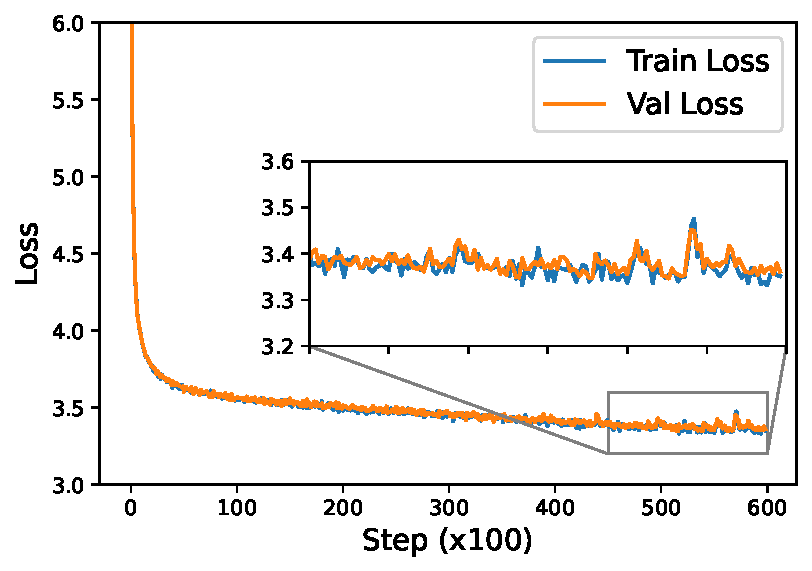
\includegraphics[width=0.5\textwidth]{\toplevelprefix/chapters/chapter7/figs/gpt-loss.pdf}
    \caption{\bf Curba de pierdere a CRATE-GPT-Base antrenat pe setul de date OpenWebText.}
    \label{fig:crate-text-evals}
\end{figure}

\paragraph{Rezultate experimentale.}

\Cref{tab:gpt-eval} demonstrează că modelele CRATE ating performanță rezonabilă la pierderea de modelare a limbajului cauzal pe o varietate de seturi de date comparativ cu modelele GPT-2 cu numere similare de parametri și arhitecturi similare.


\begin{table}
\def\arraystretch{1.1}
    \small
    \caption{\small Pierderea de entropie încrucișată zero-shot a modelului CRATE-GPT2-Base și modelelor GPT2-Small, GPT2-Base evaluate pe împărțirea de test a seturilor de date ($\downarrow$ mai mic este mai bine).
    }
    \centering
    \begin{tabular}{ccccccc}
    \hline
    & \#parametri & \textbf{OWT} & \textbf{LAMBADA} & \textbf{WikiText} & \textbf{PTB} & \textbf{Med} \\
     \hline
     GPT2-Base  & {124M} & 2.85$\downarrow$ & 4.12$\downarrow$ & 3.89$\downarrow$ & 4.63$\downarrow$ & 3.87$\downarrow$ \\
     {GPT2-Small } &  {64M} & {3.04} & {4.49} & {4.31} & {5.15} & {4.25} \\
     Causal-CRATE-Base & {60M} & 3.37 & 4.91 & 4.61 & 5.53 & 4.61 \\
     \hline
    \end{tabular}
    \label{tab:gpt-eval}
\end{table} 





























\section{Scalarea Transformerilor White-Box}\label{sec:scalable}

În această secțiune, vom discuta trei moduri în care diverse părți ale modelelor de tip CRATE pot fi scalate sau făcute mai eficiente, rămânând în același timp white-box. Aceste dezvoltări combină atât perspective conceptuale, cât și empirice, și pot fi văzute ca studii de caz despre cum să folosim înțelegerea white-box pentru a îmbunătăți modelele de învățare profundă în practică. Sarcinile pe care le folosim pentru a evalua metodele vor fi clasificarea imaginilor și predicția următorului token, datele vor fi ImageNet și OpenWebText respectiv, procedura de optimizare va fi aceeași backpropagare, iar singurul lucru care se schimbă este arhitectura.

\subsection{Creșterea Lățimii Rețelei: CRATE-\texorpdfstring{\(\alpha\)}{alpha}}\label{sub:crate_alpha_experiments}

\begin{figure}[t]
    \centering 
    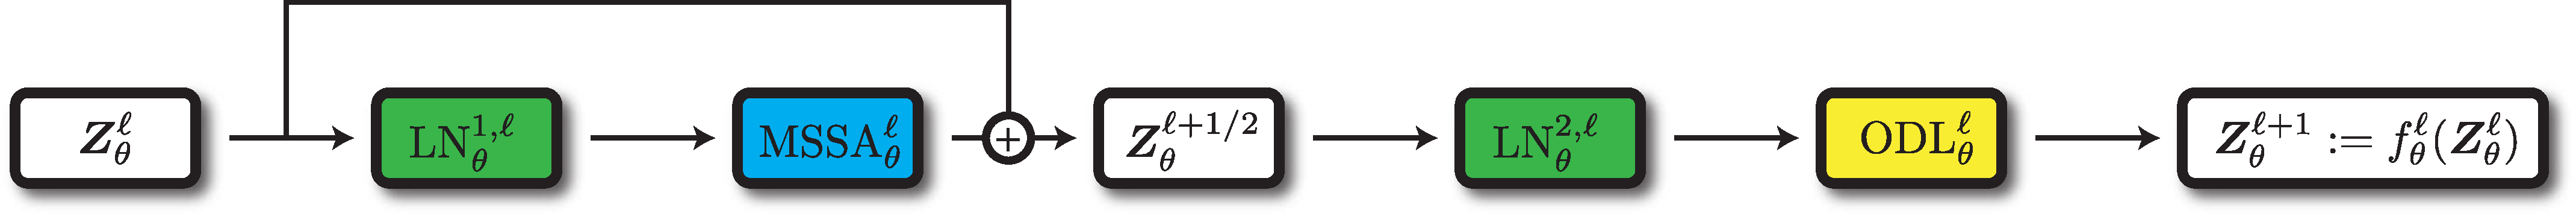
\includegraphics[width=\textwidth]{\toplevelprefix/chapters/chapter7/figs/crate_alpha_backbone.pdf}
    \caption{\small\textbf{Un strat al coloanei vertebrale CRATE-\(\alpha\).} Diferența față de CRATE este că blocul \(\ISTA_{\theta}^{\ell}\) este înlocuit cu blocul \(\operatorname{ODL}_{\theta}^{\ell}\), care efectuează mai mulți pași \(\ISTA\) cu un dicționar supracomplet.}
    \label{fig:crate_alpha_backbone}
\end{figure}


O decizie de design impusă de cadrul CRATE este \textit{lățimea} neliniarității din rețea. Într-un transformer obișnuit, lățimea este de obicei setată la \(4\), \(8\) sau \(\frac{11}{3}\) ori dimensiunea caracteristicii. Cu toate acestea, CRATE impune ca lățimea să fie exact egală cu dimensiunea caracteristicii, adică dicționarele \(\vD^{\ell}\) sunt pătrate, ceea ce ar putea duce la performanță redusă. Motivul fundamental pentru care cadrul CRATE ne constrânge la această alegere este următorul:
\begin{itemize}
    \item Blocul ISTA ia un \textit{singur} pas de optimizare pentru învățarea dicționarului.
    \item De obicei, un pas al oricărui algoritm de optimizare iterativ nu poate optimiza efectiv obiectivul. Atunci de ce funcționează acest lucru?
    \item Algoritmii de optimizare converg de obicei foarte repede dacă și numai dacă au inițializări bune sau \textit{porniri calde}. Blocul ISTA are o pornire caldă --- tratează caracteristicile de intrare ca o inițializare pentru codurile rare rezultate.
    \item Acest lucru impune ca caracteristicile de intrare și codurile rare să aibă aceeași dimensiune. Anume, ISTA învață un dicționar de rarefiere complet (cf \Cref{ch:classic}).
\end{itemize}
Astfel, dacă vrem să folosim un dicționar larg, avem nevoie ca ISTA să efectueze învățarea dicționarului \textit{supracomplet}. Aceasta înseamnă că nu putem avea aceeași pornire caldă (deoarece codurile noastre rare au o dimensiune mai mare decât caracteristicile noastre) și avem nevoie de mai multe iterații pentru a converge la un cod rar. Prin urmare, pasul de la caracteristici \(\vZ_{\theta}^{\ell + 1/2}\) la coduri rare \(\vZ_{\theta}^{\ell + 1}\) nu ar mai fi
\begin{equation}
    \vZ_{\theta}^{\ell + 1} = \ISTA_{\theta}^{\ell}(\vZ_{\theta}^{\ell + 1/2} \mid \vZ_{\theta}^{\ell + 1/2})
\end{equation}
unde funcția \(\ISTA_{\theta}^{\ell}\) este definită ca (printr-un abuz de notație din secțiunile anterioare)
\begin{equation}
    \ISTA_{\theta}^{\ell}(\vZ \mid \vY) \doteq \ReLU(\vZ - \beta (\vD^{\ell})^{\top}(\vD^{\ell}\vZ - \vY) + \beta \lambda \vone_{s}\vone_{n}^{\top})
\end{equation}
ci mai degrabă următoarea iterație:
\begin{equation}
    \vZ_{\theta}^{\ell + 1} = \vA_{\theta}^{\ell, T}; \qquad \vA_{\theta}^{\ell, t + 1} = \ISTA_{\theta}^{\ell}(\vA_{\theta}^{\ell, t} \mid \vZ_{\theta}^{\ell + 1/2}) \quad \forall 0 \leq t < T; \qquad \vA_{\theta}^{\ell, 0} = \vzero_{s \times n},
\end{equation}
adică, rulând gradient proximal pe obiectivul LASSO pentru \(T \geq 1\) pași în trecerea înainte la fiecare strat, inițializat la \(\vzero_{s \times n}\). În această circumstanță, dicționarul poate fi atât de larg cât este necesar, adică, \(\vD^{\ell} \in \R^{s \times d}\) unde \(s \geq d\) (de obicei se ia \(s = 4d\) în practică).

\begin{table}[b]
    \centering
    \begin{tabular}{@{}lcccccccc@{}}
    \toprule
     &  & \multicolumn{3}{c}{Detecție} &  \multicolumn{3}{c}{Segmentare} \\ 
    Model & AP$_{50} \uparrow $ & AP$_{75} \uparrow $ & AP $\uparrow$ & AP$_{50} \uparrow$ & AP$_{75} \uparrow $ & AP $\uparrow$ \\ 
    \midrule
    \midrule
    CRATE-\(\alpha\)-B/8 & 3.5 & 1.1 & 1.5 & 2.2 & 1.0 & 1.1 \\
    CRATE-\(\alpha\)-L/8 & \textbf{4.0} & \textbf{1.7} & \textbf{2.0} & \textbf{2.7} & \textbf{1.1} & \textbf{1.4} \\
    \midrule
    \color{gray}CRATE-B/8 & \color{gray}2.9 & \color{gray}1.0 & \color{gray}1.3 & \color{gray}2.2 & \color{gray}0.7 & \color{gray}1.0 \\
    \color{gray}ViT-B/8 & \color{gray}0.8 & \color{gray}0.2 & \color{gray}0.4 & \color{gray}0.7 & \color{gray}0.5 & \color{gray}0.4 \\
    \bottomrule
    \end{tabular}
    \caption{\small \textbf{Detecția obiectelor și segmentarea fină prin MaskCut pe COCO val2017~\citep{lin2014microsoft}}. Aici toate modelele sunt antrenate cu dimensiunea patch-ului \(8\) în loc de \(16\). Comparativ cu modelele existente precum CRATE și ViT, familia de modele CRATE-\(\alpha\) are în mod notabil performanță îmbunătățită precum și scalabilitate.}
    \label{tab:crate_alpha_detection_segmentation}
\end{table}

Cu toate acestea, acest lucru prezintă o problemă empirică. Folosind configurația de mai sus, dacă \(\vZ^{\ell + 1/2} \in \R^{d \times n}\), atunci \(\vZ^{\ell + 1} \in \R^{s \times n}\), care poate avea o dimensiune a caracteristicii arbitrar de mare. În practică, vrem ca dimensiunea caracteristicii la fiecare strat să fie aceeași. Deci acest lucru stabilește o trihotomie practică pentru proiectarea rețelei, anume, \textit{nu putem} avea \textit{toate} următoarele deziderate:
\begin{enumerate}
    \item Dimensiunea caracteristicii la fiecare strat este aceeași.
    \item Dicționarul este larg, adică supracomplet.
    \item Ieșirea neliniarității sunt codurile rare ale intrării în raport cu dicționarul.
\end{enumerate}
În practică, renunțarea la (1) este mai puțin tractabilă din motive de eficiență. Renunțarea la (2) duce la cadrul CRATE obișnuit. Renunțarea la (3) duce la o versiune largă a CRATE, adică CRATE-\(\alpha\), care are următoarea neliniaritate pentru a obține de la \(\vZ^{\ell + 1/2}\) la \(\vZ^{\ell + 1}\):
\begin{equation}
    \vZ_{\theta}^{\ell + 1} = \vD^{\ell}\vA_{\theta}^{\ell, T}; \qquad \vA_{\theta}^{\ell, t + 1} = \ISTA_{\theta}^{\ell}(\vA_{\theta}^{\ell, t} \mid \vZ_{\theta}^{\ell + 1/2}); \qquad \vA_{\theta}^{\ell, 0} = \vzero,
\end{equation}
adică, ia codurile rare obținute prin gradient descendent proximal și înmulțește cu dicționarul pentru a obține versiunea denoisificată a intrării. Astfel, neliniaritatea CRATE-\(\alpha\) calculează o versiune denoisificată a intrării care este amenabilă codării rare, nu codurile rare propriu-zise. Harta de la \(\vZ_{\theta}^{\ell + 1/2}\) la \(\vZ_{\theta}^{\ell + 1}\) aici se numește blocul de Învățare a Dicționarului Supracomplet (ODL) și este notată \(\operatorname{ODL}_{\theta}^{\ell}\), adică,
\begin{equation}
    \vZ_{\theta}^{\ell + 1}(\vX) \doteq \operatorname{ODL}_{\theta}^{\ell}(\vZ_{\theta}^{\ell + 1/2}(\vX)).
\end{equation}



\begin{figure}[t]
    \centering 
    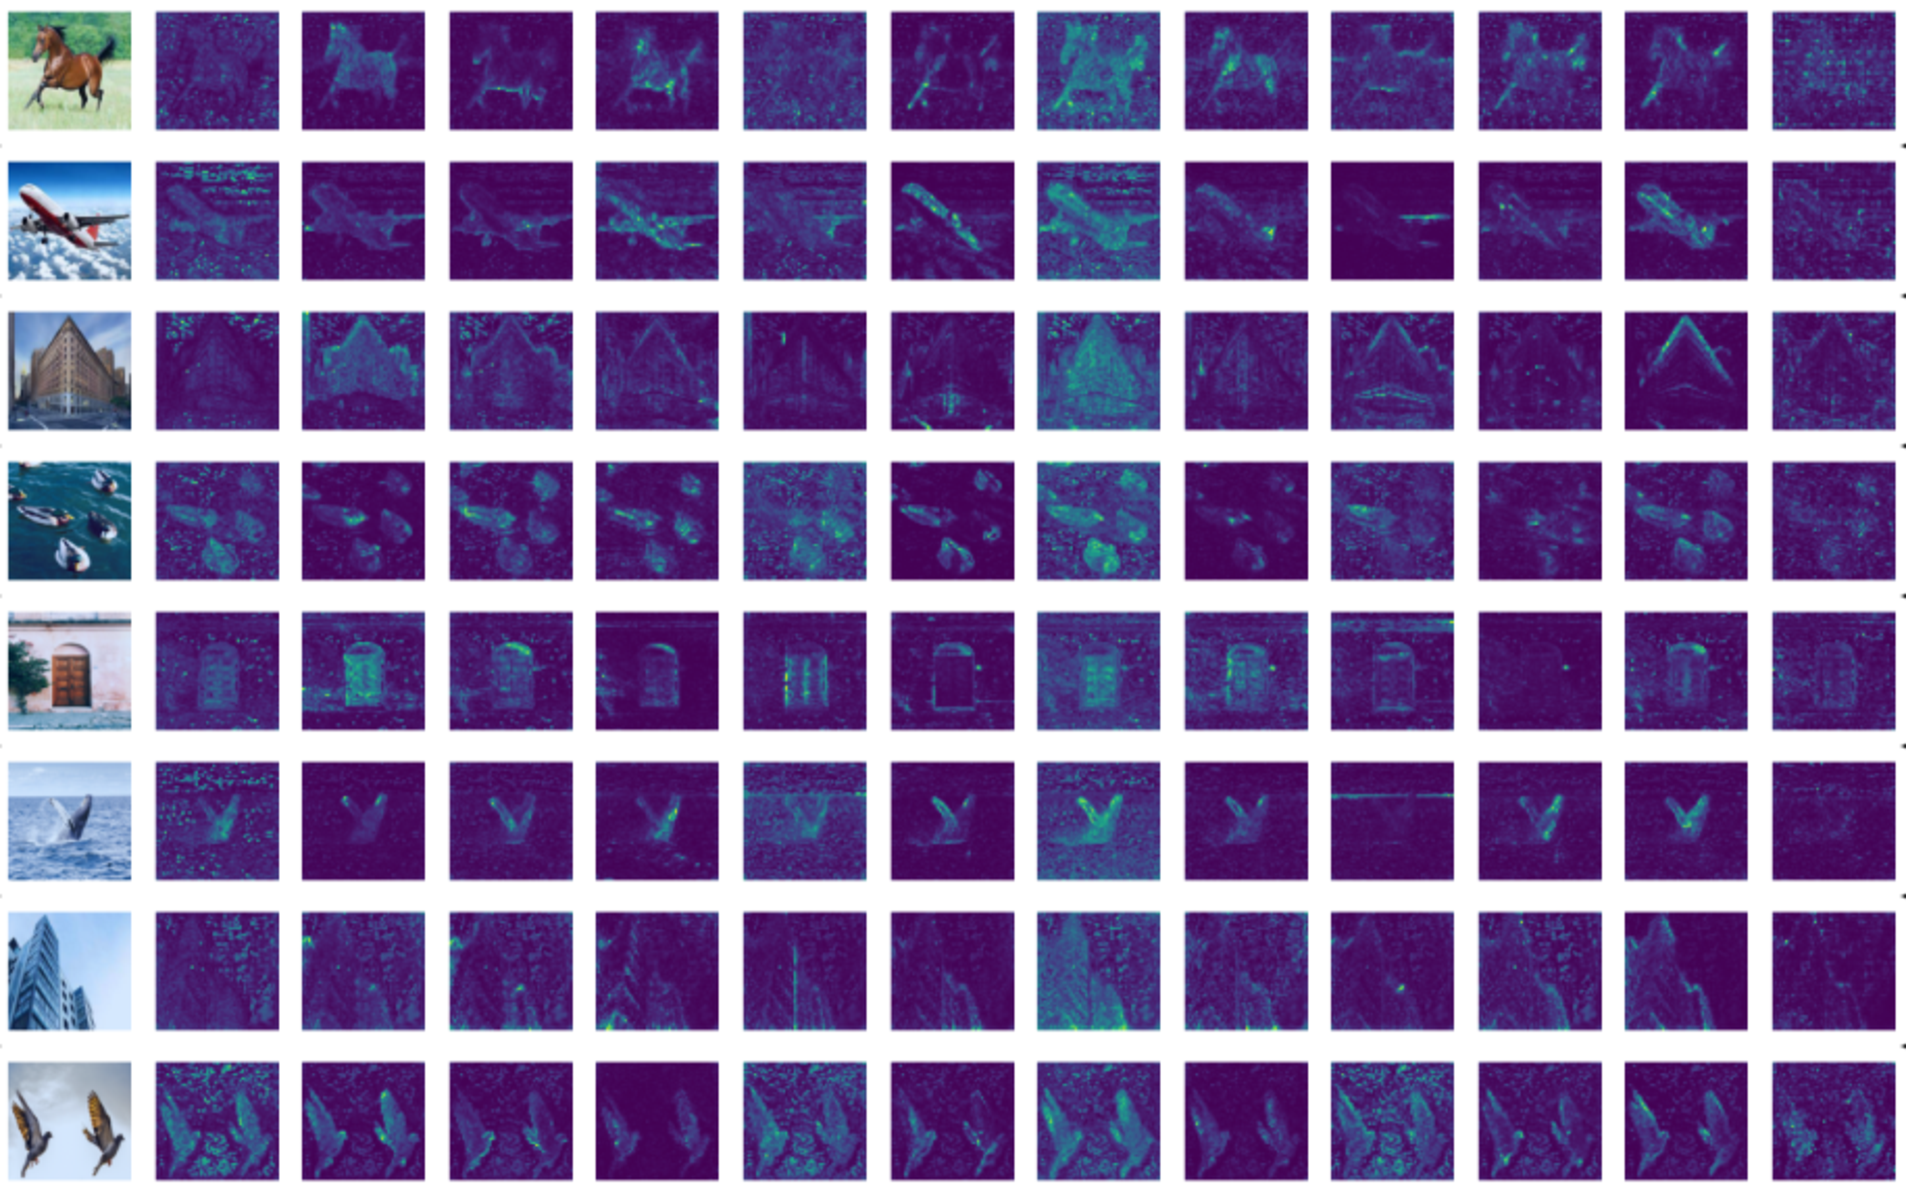
\includegraphics[width=\textwidth]{\toplevelprefix/chapters/chapter7/figs/crate_alpha_semantic_heads.pdf}
    \caption{\small\textbf{Hărți de saliență de la CRATE-\(\alpha\) cu dimensiunea patch-ului \(8\).} Fiecare rând este o imagine diferită și fiecare coloană corespunde unui cap de atenție diferit în ultimul strat. Observăm că hărțile de saliență corespund puternic obiectelor din imaginea de intrare.}
    \label{fig:crate_alpha_saliency_maps}
\end{figure}



\begin{table}
    \centering 
    \begin{tabular}{@{}lcccc@{}}
    \toprule
    Model & GPT-2-B(ază) & CRATE-B & CRATE-\(\alpha\)-S(mic) & CRATE-\(\alpha\)-B \\ 
    \midrule
    \midrule
    \# parametri & 124M & 60M & 57M & 120M \\
    Pierd. val. OWT & 2.85 & 3.37 & 3.28 & 3.14 \\
    \bottomrule
    \end{tabular}
    \caption{\small\textbf{Pierderea de validare în modelarea limbajului.} Aici toate modelele sunt pre-antrenate pe majoritatea OpenWebText, iar pierderea de entropie încrucișată de validare este măsurată pe un subset holdout al OpenWebText. CRATE-\(\alpha\) arată o îmbunătățire semnificativă față de designul CRATE, deși încă există un decalaj cu transformerii tradiționali precum GPT-2.}
    \label{tab:crate_alpha_lm}
\end{table}

Stratul CRATE-\(\alpha\) este prezentat în \Cref{fig:crate_alpha_backbone}. În practică, această modificare a CRATE performează foarte bine la scale mai mari. De exemplu, când pre-antrenăm modele CRATE-\(\alpha\) pe ImageNet-21K, sarcinile nesupervizate precum segmentarea (vezi \Cref{fig:crate_alpha_saliency_maps} și \Cref{tab:crate_alpha_detection_segmentation}) au în general performanță semnificativ îmbunătățită comparativ cu CRATE. Tendințe similare sunt prezente în antrenamentul modelului de limbaj folosind auto-atenție cauzală (vezi \Cref{tab:crate_alpha_lm}). În general, este o cale promițătoare pentru scalarea performanței pentru a egala modelele black-box precum transformerii.\footnote{Rețineți că rezultatele experimentale din această secțiune folosesc o arhitectură de model ușor diferită, care adaugă câștiguri empirice foarte ușoare. Modificările sunt: (1) o conexiune reziduală suplimentară pe blocul ODL, (2) modificarea \(\ISTA\) pentru a folosi două dicționare separate în loc de \(\vD^{\ell}\) și \((\vD^{\ell})^{\top}\).}


\subsection{Transformeri cu Complexitate de Timp Liniară}\label{sub:tost_experiments}

În practică, modelele de învățare profundă suferă de blocaje în complexitatea spațiului și timpului, reprezentând dimensiuni ale problemei dincolo de care nu pot scala date resursele fixe. Un astfel de blocaj, deosebit de semnificativ când se ocupă cu date unde fiecare mostră este ea însăși de dimensiune înaltă și bogată (cum ar fi fluxuri lungi de text sau videoclipuri), este \textit{complexitatea de timp} a procesării secvențelor lungi de date. Pentru a atenua complexitatea de timp a procesării datelor folosind transformeri, în \Cref{sub:tost} am propus un operator \textit{auto-atenție cu statistici de token} \(\TSSA_{\theta}^{\ell}\). Acum construim un \textit{transformer cu statistici de token}, numit ToST, în jurul acestuia, pe care îl putem folosi pentru sarcini cu context lung. În special, putem folosi următorul strat (ilustrat în \Cref{fig:tost_backbone}) ca înlocuitor direct pentru un strat de coloană vertebrală în CRATE:
\begin{align}
    \vZ_{\theta}^{\ell + 1/2}(\vX)
    &= \vZ_{\theta}^{\ell}(\vX) + \TSSA_{\theta}^{\ell}(\LN_{\theta}^{1, \ell}(\vZ_{\theta}^{\ell}(\vX))) \\ 
    \vZ_{\theta}^{\ell + 1}(\vX)
    &= \vZ_{\theta}^{\ell + 1/2}(\vX) + \MLP_{\theta}^{\ell}(\LN_{\theta}^{2, \ell}(\vZ_{\theta}^{\ell + 1/2}(\vX)))
\end{align}
unde blocul \(\TSSA\) este definit ca în \Cref{sub:tost}. Observați că aceasta este exact aceeași cu arhitectura vision transformer discutată în \Cref{sub:contrastive_learning_architecture}, cu excepția faptului că \(\TSSA\) înlocuiește blocul convențional de auto-atenție multi-cap \(\MHSA\). Indiferent, complexitatea computațională a trecerii înainte a acestui strat este liniară în toate variabilele problemei --- lungimea secvenței, dimensiunea caracteristicii, numărul de capete și dimensiunea capului.

\begin{figure}[!htbp]
    \centering 
    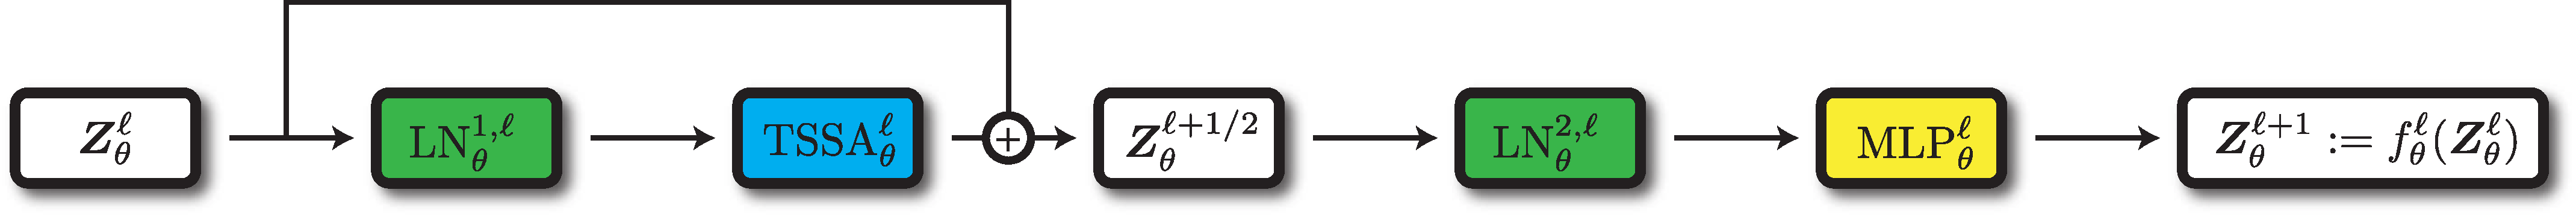
\includegraphics[width=\textwidth]{\toplevelprefix/chapters/chapter7/figs/tost_backbone.pdf}
    \caption{\small\textbf{Un strat al coloanei vertebrale ToST}. Reprezentările token trec prin normalizări de strat, operatorul de auto-atenție cu statistici de token (TSSA) și un MLP, pentru a forma ieșirea stratului.}
    \label{fig:tost_backbone}
\end{figure}

\begin{table}[t]
    \centering 
    \resizebox{\textwidth}{!}{
    \begin{tabular}{@{}lccc|cc|cc@{}}
    \toprule
    Seturi de date & ToST-T(mic) & ToST-S(mic) & ToST-M(ediu) &  { \color{gray} XCiT-S} &  { \color{gray}XCiT-M} &  {\color{gray}ViT-S} & {\color{gray}ViT-B(ază)}\\ 
    \toprule
     \# parametri & 5.8M & 22.6M & 68.1M &  { \color{gray}24.9M }& { \color{gray}80.2M } & { \color{gray} 22.1M } & { \color{gray}86.6 M } \\
    \midrule
     ImageNet & 67.3 & 77.9 & 80.3 &  { \color{gray} 80.5} & { \color{gray} 81.5 } & { \color{gray} 79.8} & { \color{gray} 81.8} \\
     ImageNet ReaL & 72.2  & 84.1 & 85.6 &  { \color{gray} 85.6 } & { \color{gray} 85.9} & { \color{gray} 85.6 } & { \color{gray} 86.7 }\\
     \midrule
     CIFAR10 & 95.5 & 96.5 & 97.5 &  { \color{gray} 98.1} & { \color{gray} 98.3} & { \color{gray} 98.6} & { \color{gray} 98.8}\\
     CIFAR100 & 78.3 & 82.7 & 84.5 &  { \color{gray} 86.1} & { \color{gray} 87.6} & { \color{gray} 88.8} & { \color{gray} 89.3}\\
     Oxford Flowers-102 & 88.6 & 92.8 & 94.2 &  { \color{gray} 93.9} & { \color{gray} 94.0} & { \color{gray} 94.0}& { \color{gray} 95.7}\\
     Oxford-IIIT-Pets & 85.6 & 91.1 & 92.8 &  { \color{gray} 92.9} & { \color{gray} 94.0} & { \color{gray} 92.8} & { \color{gray} 94.1} \\
     \bottomrule
    \end{tabular}%
    }
    \caption{\small \textbf{Acuratețea clasificării prin sondare liniară a ToST} pe diverse seturi de date cu diferite dimensiuni de model când coloana vertebrală este pre-antrenată pentru clasificare ImageNet-1K. Observăm că, comparativ cu XCiT (o arhitectură de tip transformer proiectată empiric specializată pentru procesarea eficientă a secvențelor lungi) și ViT, ToST menține performanță relativ similară, chiar și bucurându-se de beneficii precum timp de rulare mai rapid și design white-box.}
    \label{tab:tost_linear_probing}
\end{table}

\begin{table}[!htbp]
    \centering 
    \begin{tabular}{@{}lcccccc@{}}
        \toprule
        Model & \# param & OWT & Lambada & Wikitext & PTB & Med $\downarrow$ \\ \midrule
        GPT-2-Base & 124M & 2.84 & 4.32 & 4.13 & 5.75 & 4.26 \\
        ToST-Base & 110M & 3.20 & 4.98 & 4.77 & 6.39 & 4.84 \\
        ToST-Medium & 304M & 2.88 & 4.45 & 4.30 & 5.64 & 4.32 \\
        ToST-Large & 655M & 2.72 & 4.32 & 3.99 & 5.03 & 4.02 \\ \bottomrule
    \end{tabular}%
    \caption{\small\textbf{Pierderea de validare a modelării limbajului} calculată pe (seturi holdout ale) unei varietăți de seturi de date de limbaj natural, după pre-antrenarea modelului pe acel set de date. Observăm că ToST scalează bine, astfel încât ToST-Large depășește GPT-2-Base de bază în modelarea limbajului cauzal, bucurându-se în același timp de eficiență superioară în contexte lungi.}
    \label{tab:tost_lm}
\end{table}

\begin{table}
    \centering
    
    \begin{tabular}{@{}lccccccc@{}}
            \toprule
            Model        & ListOps  & Text     & Regăsire & Imagine    & Pathfinder & Medie      \\
            \midrule
            \midrule
            Reformer              & \textbf{37.27} & 56.10             & 53.40              & 38.07             & 68.50               & 50.56             \\
            BigBird               & 36.05             & 64.02             & 59.29              & 40.83             & 74.87                & 54.17             \\
            LinFormer         & 16.13             & \underline{65.90} & 53.09              & 42.34             & \underline{75.30}               & 50.46             \\
            Performer             & 18.01             & 65.40             & 53.82              & 42.77             & \textbf{77.05}                & 51.18             \\
            Transformer           & 37.11             & 65.21             & \underline{79.14}              & \underline{42.94}             & 71.83              & \underline{59.24}            \\
            ToST & \underline{37.25}    & \textbf{66.75}    & \textbf{79.46}     & \textbf{46.62}    &    69.41      &     \textbf{59.90}\\
            
            \bottomrule
        \end{tabular}%
    \caption{\small \textbf{Comparația performanței Long-Range Arena (LRA) a ToST(-B) versus cele mai bune variante de transformer optimizate pentru context lung.} Long-Range Arena este o familie de teste de referință care testează capacitatea de modelare a secvențelor lungi a algoritmilor și arhitecturilor, prin fixarea setului de date și a mecanismului de evaluare. ToST obține scoruri de top în clasament comparativ cu toate variantele cunoscute de transformer, inclusiv XCiT și transformer-ul regular (ViT) (cf. \Cref{tab:tost_linear_probing}). Mai mult, ToST are cea mai mică complexitate de timp și spațiu la inferență. (În acest tabel, cel mai bun scor pentru un anumit test de referință este îngroșat, iar al doilea cel mai bun scor este subliniat.)}
    \label{tab:tost_lra_results}
\end{table}

Mai mult, arhitectura propusă, numită ToST (pentru ``Token Statistics Transformer'') performează bine la sarcini de viziune (adică, \Cref{tab:tost_linear_probing}) și sarcini de limbaj (adică, \Cref{tab:tost_lm}). Acest lucru este valabil în special pentru sarcinile cu lungime mare de secvență (cf. \Cref{tab:tost_lra_results}), unde este atât mai performantă, cât și mult mai eficientă decât transformer-ele convenționale și toate celelalte arhitecturi de tip transformer.

\subsection{Transformere doar cu atenție} \label{sub:aot_experiments}

Un alt blocaj de eliminat din modelele de învățare profundă, în special din arhitecturile de tip transformer, este blocajul de memorie care provine din înmulțirile masive de matrici în MLP-uri, unde dimensiunea internă este cu mult mai mare decât dimensiunea caracteristicilor \(d\). Astfel, este o întrebare interesantă și importantă de pus: avem \textit{într-adevăr} nevoie de MLP în interiorul unui transformer și cât de bună poate fi performanța fără el? Pentru a explora această întrebare, folosim arhitectura transformer-doar-cu-atenție (AoT) (vezi \Cref{sub:aot}), ilustrată în \Cref{fig:aot_backbone}. Mai exact, fiecare strat este pur și simplu de forma 
\begin{equation}
    \vZ_{\theta}^{\ell + 1}(\vX) = \vZ_{\theta}^{\ell}(\vX) + \MSSA_{\theta}^{\ell}(\LN_{\theta}^{\ell}(\vZ_{\theta}^{\ell}(\vX))).
\end{equation}
În implementarea noastră, am experimentat și cu utilizarea auto-atenției multi-cap (MHSA) în locul MSSA. Se dovedește că această arhitectură este \textit{de asemenea} viabilă, deși adâncimea rețelei trebuie să fie mult mai mare pentru a obține performanță echivalentă cu arhitectura obișnuită CRATE sau transformer. %

\begin{figure}[!htbp]
    \centering 
    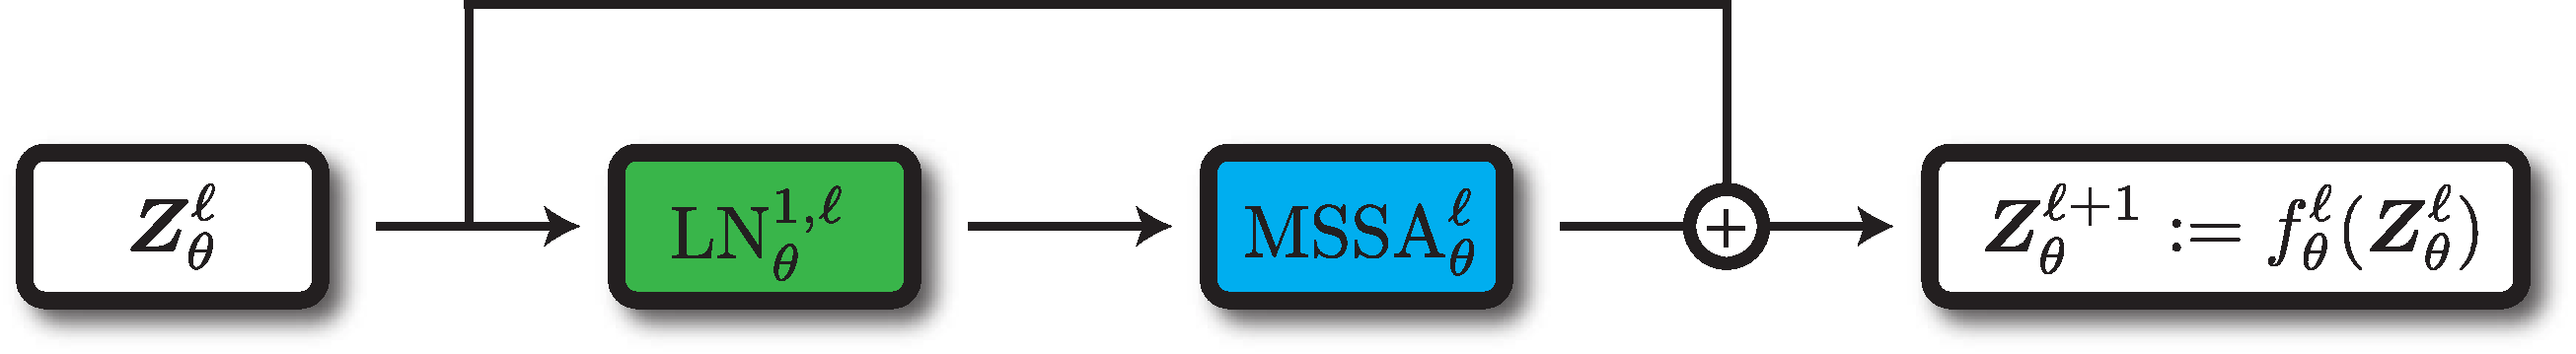
\includegraphics[width=0.7\textwidth]{\toplevelprefix/chapters/chapter7/figs/aot_backbone.pdf}
    \caption{\small\textbf{Un strat al backbone-ului AoT.} Reprezentările token-urilor trec doar printr-o normalizare pe straturi și operatorul de auto-atenție multi-cap (subspațiu) pentru a forma ieșirea stratului. Observați că nu există neliniaritate la nivel de token precum MLP sau ISTA sau ODL.}
    \label{fig:aot_backbone}
\end{figure}


Efectuăm experimente folosind arhitectura AoT propusă și demonstrăm potențialul acesteia. Pre-antrenăm modelele AoT-MSSA și AoT-MHSA de diferite dimensiuni, împreună cu GPT-2, pe OpenWebText~\citep{Gokaslan2019OpenWeb}. Reprezentăm grafic pierderea de antrenare și pierderea de validare în funcție de numărul de iterații de antrenare în \Cref{fig:loss}(a) și, respectiv, (b). Se observă că modelele bazate pe AoT de dimensiuni medii și mari obțin pierderi de antrenare și validare comparabile cu cele ale modelului de bază GPT-2. În plus, comparativ cu modelul de bază GPT-2, modelul AoT-MHSA este identic cu modelul de bază GPT-2, cu excepția absenței straturilor MLP din arhitectură. După cum se arată în \Cref{fig:loss}, încorporarea straturilor MLP poate accelera procesul de antrenare. Folosind modelele pre-antrenate de mai sus, calculăm pierderea de validare cu entropie încrucișată fără antrenare pe diferite seturi de date în \Cref{tab:zeroshot}. Se observă că modelele AoT cu dimensiuni medii și mari de parametri pot obține performanță comparabilă cu modelul de bază GPT-2. Mai mult, am constatat că adăugarea straturilor MLP la AoT nu îmbunătățește performanța zero-shot. Aceste rezultate evidențiază potențialul modelelor doar-cu-atenție de a obține rezultate competitive menținând în același timp interpretabilitatea.  

\begin{table*}[!htbp]
\caption{Rezultate zero-shot pe mai multe seturi de date și sarcini de referință pentru limbaj: Evaluarea diferitelor dimensiuni de AoT cu operatorii MSSA și MHSA și comparație cu modelul GPT2.}\vskip 0.1in
\centering
\begin{small}
\begin{tabular}{l|cccccc}
\toprule
 Models  & {\bf LAMBADA} & {\bf PTB} & {\bf WikiText} & {\bf LAMBADA} & {\bf CBT CN} & {\bf CBT NE} \\
 \# of parameters  & (val loss) $\downarrow$ &  (val loss) $\downarrow$ &(val loss) $\downarrow$ & (acc) $\uparrow$ &(acc) $\uparrow$ &(acc) $\uparrow$ \\
 \midrule
 AoT-MSSA Base (102M) & 4.70 & 6.03 & 4.65 & 0.25 & 0.80 & 0.74\\
 AoT-MSSA Medium (182M) & 4.47 & 5.08 & 4.22 & 0.29 & 0.84 & 0.77 \\
 AoT-MHSA Base (122M) & 4.42 & 5.52 & 4.19 & 0.38 & 0.86 & 0.82\\
 GPT-2 Base (124M) & 4.32 & 5.75 & 4.13 &  0.40 &  0.87 &  0.84 \\
\bottomrule
\end{tabular}
\label{tab:zeroshot}
\end{small}
\end{table*} 
\vspace{-0.05in} 


\begin{figure*}[t]
\begin{center}
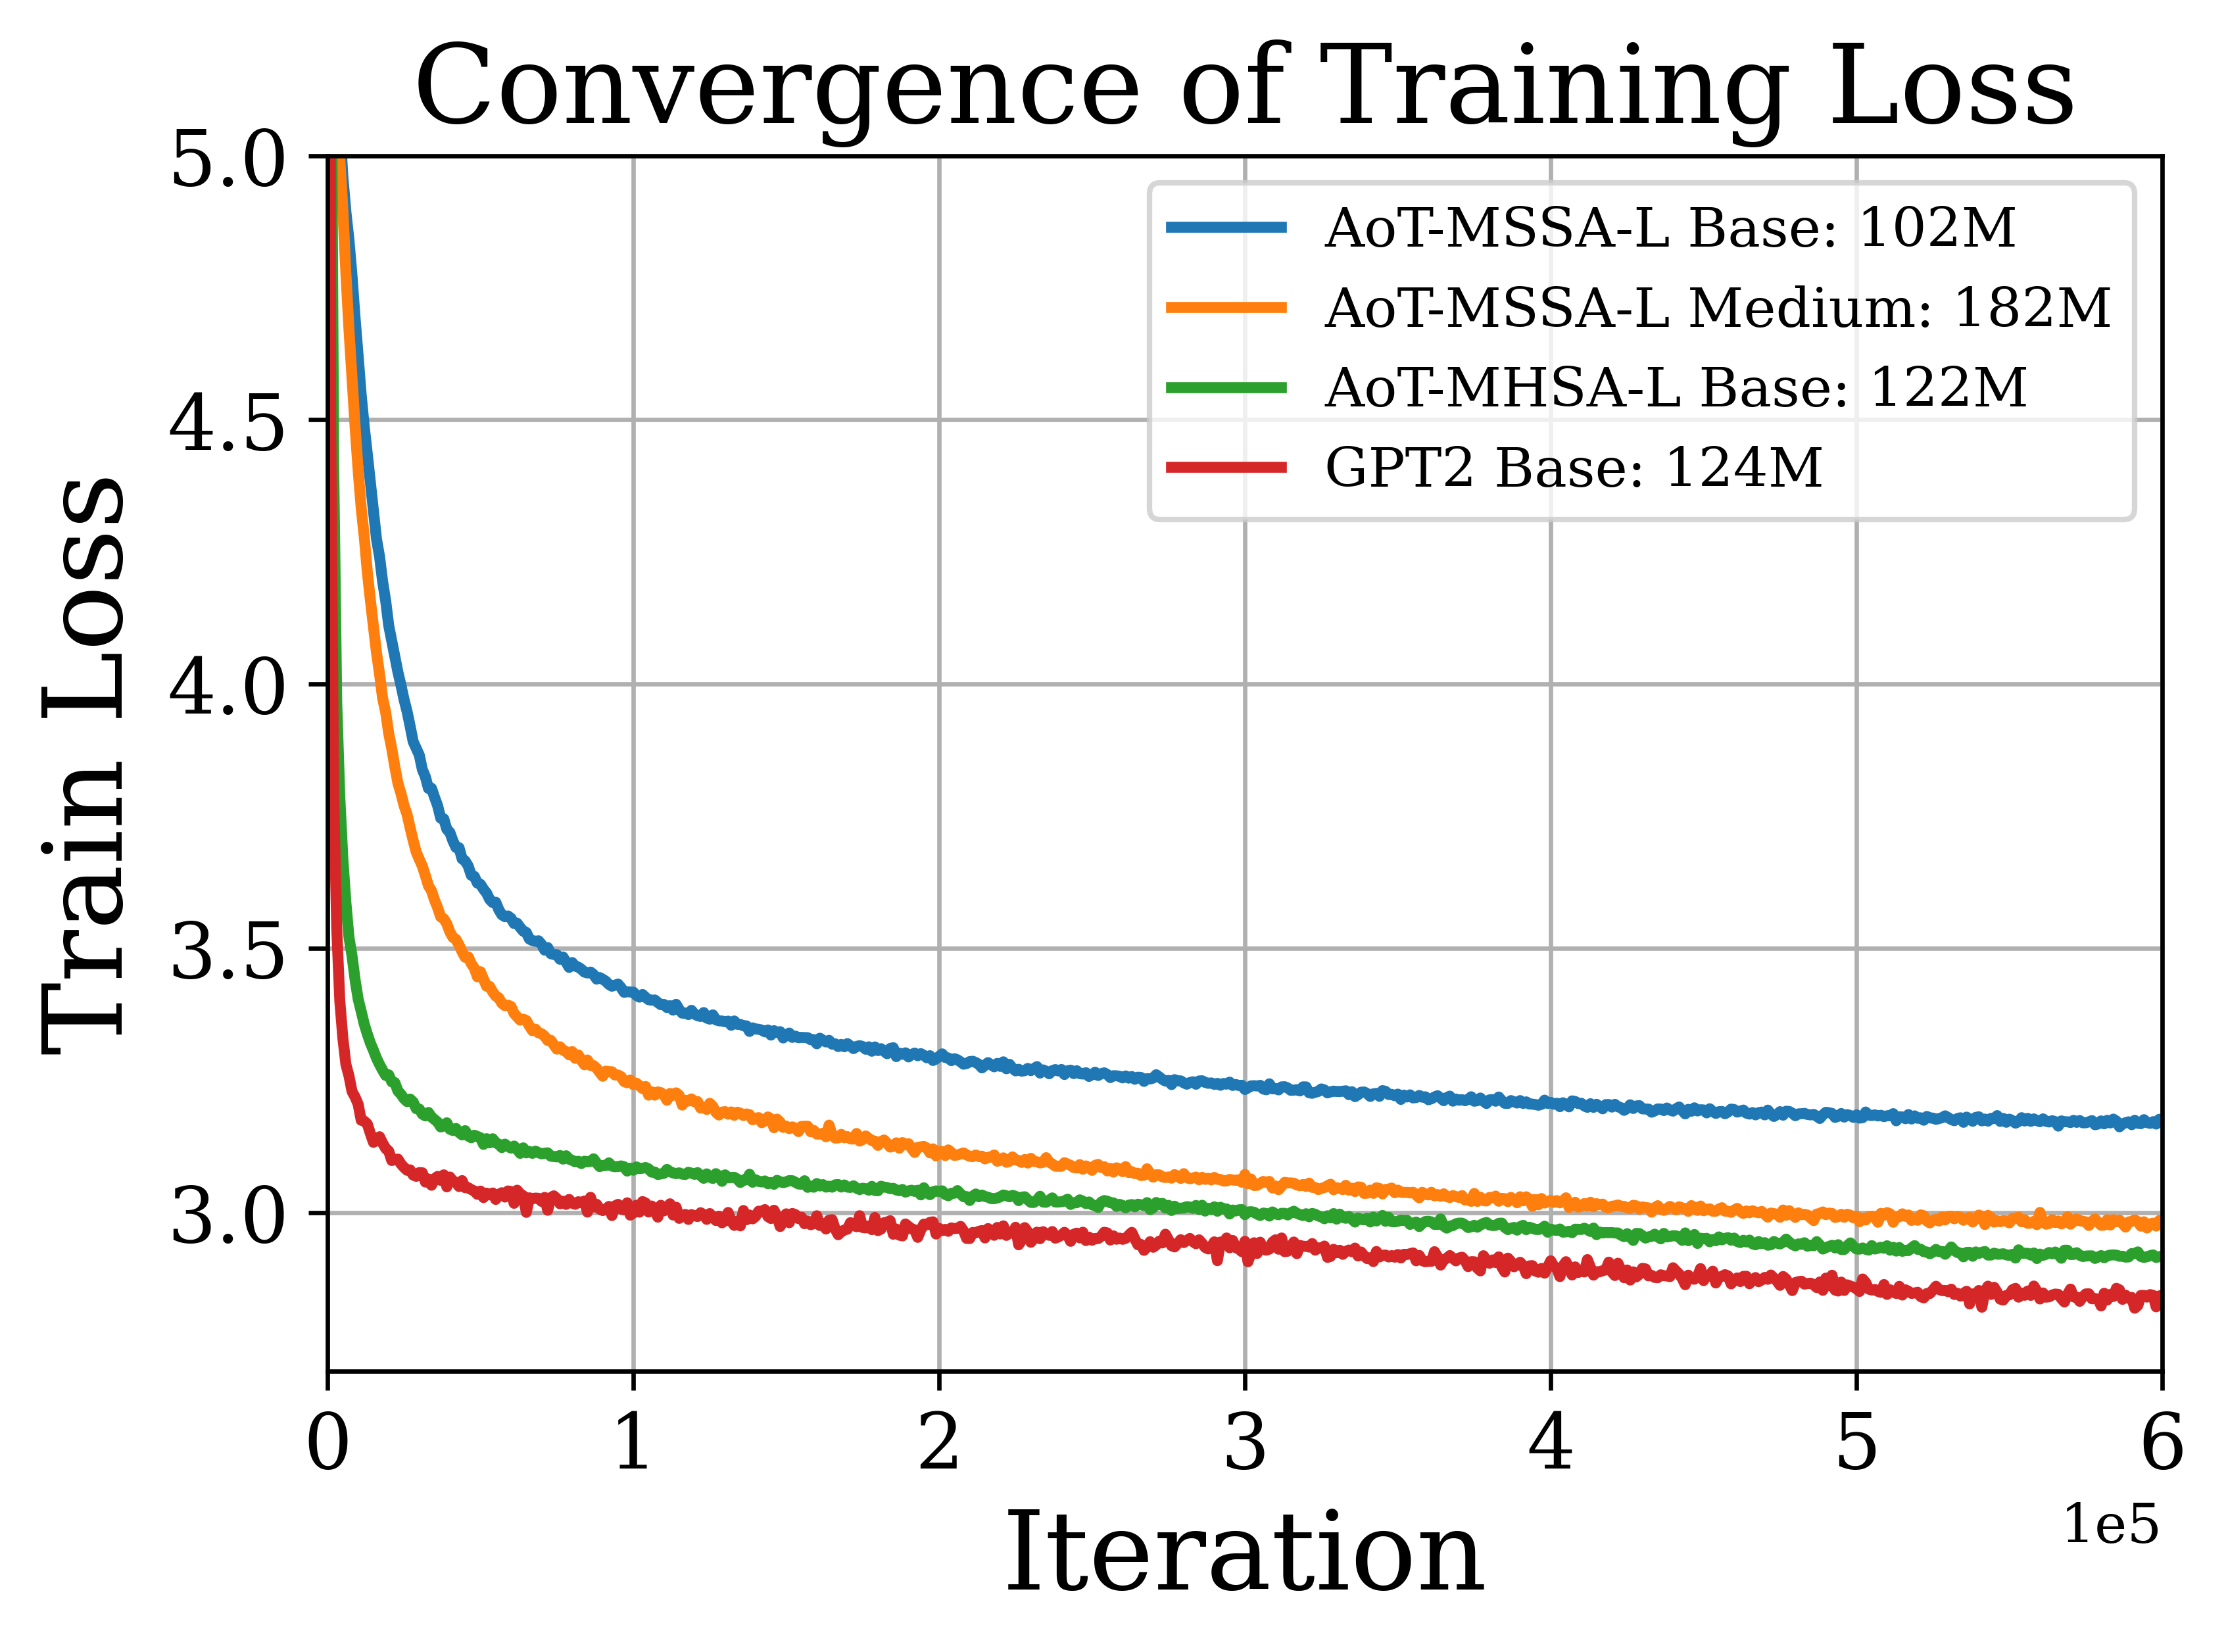
\includegraphics[width=0.4\linewidth]{\toplevelprefix/chapters/chapter7/figs/training_loss.png} \hspace{0.4in}
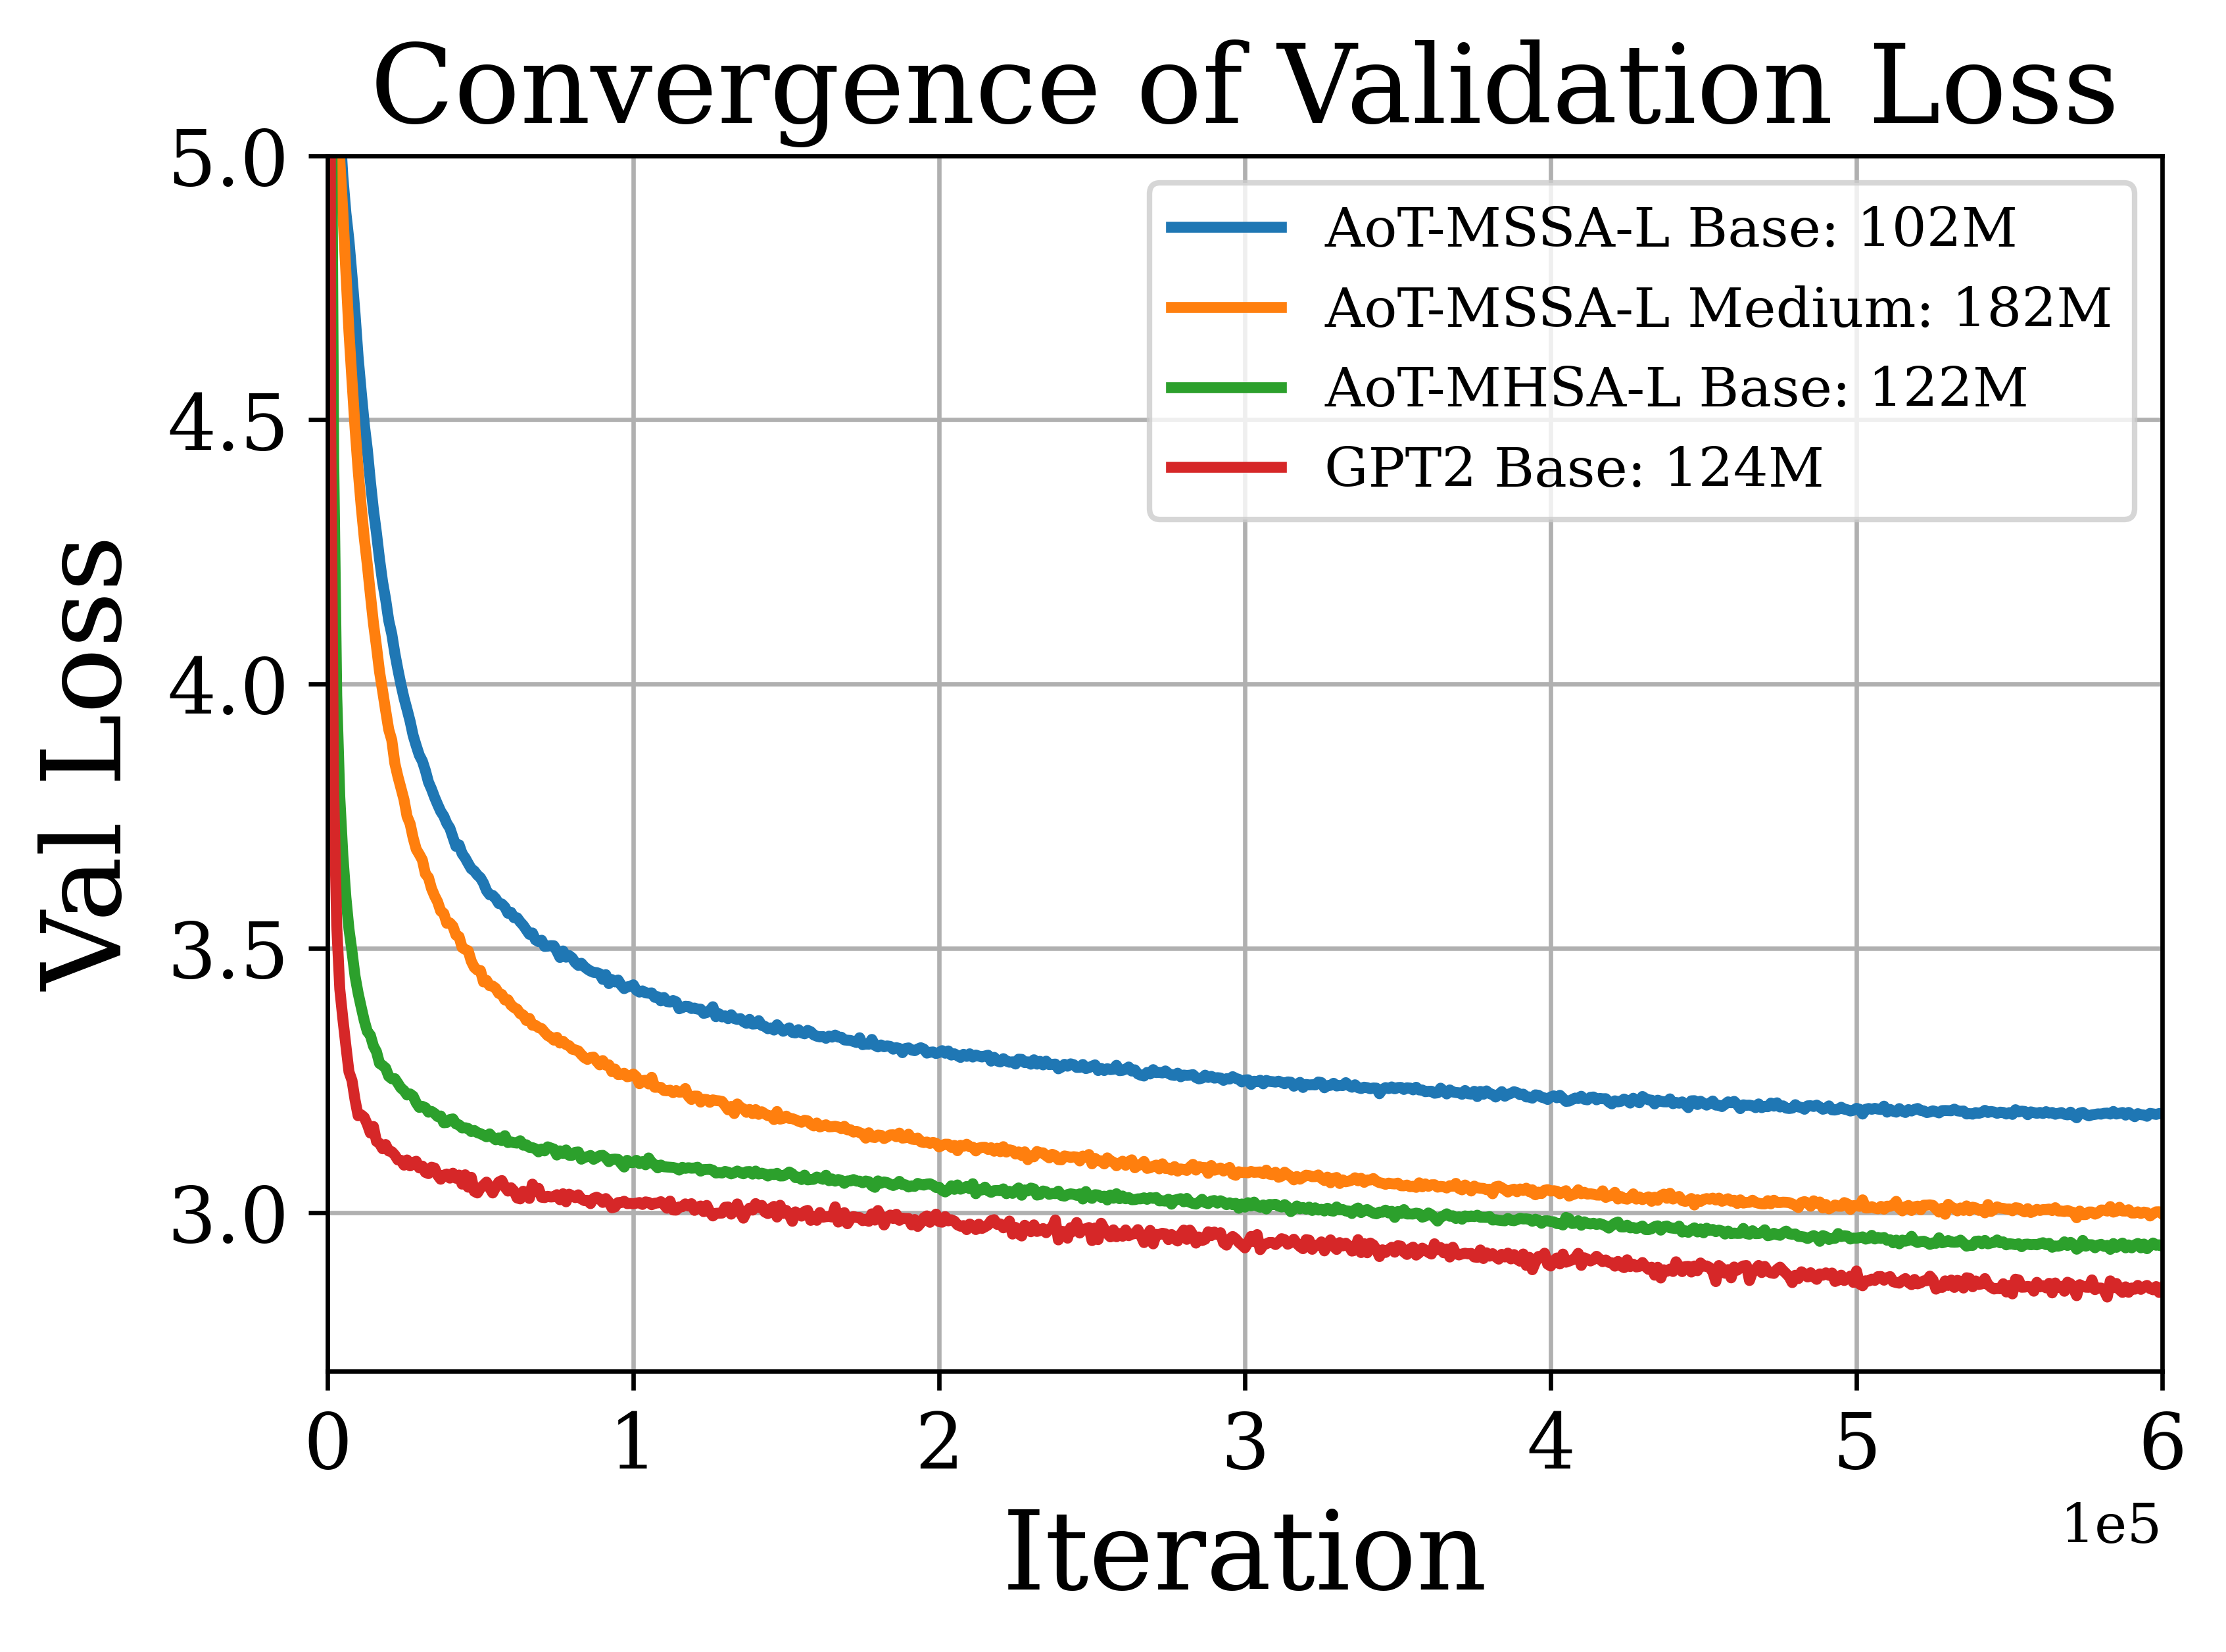
\includegraphics[width = 0.4\linewidth]{\toplevelprefix/chapters/chapter7/figs/val_loss.png}
    \vspace{-0.15in}
\caption{\centering \textbf{Evaluarea modelelor pe sarcini de limbaj.} Reprezentăm grafic pierderea de antrenare (stânga) și pierderea de validare (dreapta) a modelelor AoT și GPT-2 pre-antrenate pe OpenWebText.}  \label{fig:loss} 
\end{center}
\vspace{-0.15in}
\end{figure*} 




 

\section{Autocodare cu măscări pentru date de imagini}\label{sec:image_completion}

A doua aplicație pe care o discutăm este \textit{completarea neliniară a imaginilor}, cunoscută și sub numele de \textit{autocodare cu măscări} (MAE), care este o generalizare directă a problemei de completare a matricilor de rang mic discutată în \Cref{ch:classic}. Autocodarea cu măscări, de la introducerea sa în contextul învățării profunde de către \cite{he2022masked}, a fost o metodă de bază și simplă de învățare a reprezentărilor auto-supervizată, care își propune să înzestreze fiecare caracteristică de patch din \(\vZ_{\theta}\) cu informații agregate, precum și cu informații despre vecinii săi, astfel încât atât caracteristica patch-ului, cât și caracteristicile agregate să fie surse bogate de informații pentru întreaga probă. 

Setul de date este păstrat la fel ca seturile de date de imagini discutate în \Cref{sub:contrastive_learning_data}. Ca de obicei, aplicăm în continuare augmentări de date la fiecare probă din fiecare batch nou. 

\subsection{Sarcină și obiectiv}\label{sub:image_completion_objective}

După cum sugerează numele, autocodarea cu măscări implică o vedere \(v_{m}\) care, având o intrare, efectuează o decupare redimensionată aleatorie (cf. \Cref{sub:contrastive_learning_objective}) pentru a transforma imaginea de intrare într-o imagine pătrată de dimensiune \((C, S_{\mask}, S_{\mask})\), apoi \textit{maschează} (adică setează la zero) un procent fix \(p_{\mask} \in [0, 1]\) de pixeli din intrare. Din motive de eficiență\footnote{Implementarea originală a MAE de către \cite{he2022masked} încorporează întreaga imagine, \textit{elimină} token-urile care ar fi mascate, trece setul de token-uri rezultat prin encoder, adaugă înapoi token-uri de substituție învățate în locurile mascate și adaugă înapoi codarea pozițională corespunzătoare, și trece setul de token-uri rezultat prin decoder pentru a obține predicția de autocodare. Aceasta este mai eficientă deoarece encoder-ul are mai puține token-uri de procesat, dar conceptual este aceeași cu metoda discutată în text, iar performanța modelelor rezultate în sarcina de autocodare cu măscări și evaluările ulterioare este foarte similară.}, mascarea se face pe patch-uri, adică după încorporarea întregii imagini, un procent \(p_{\mask}\) de \textit{patch-uri} sunt setate la zero. Scopul MAE este de a antrena un encoder \(f_{\theta} \colon \cI \to (\R^{d})^{*}\) și un decoder \(g_{\eta} \colon (\R^{d})^{*} \to \cI\) care pot reconstrui o intrare din mascarea sa, adică scriind \(\hat{\vX}_{\theta, \eta} \doteq g_{\eta} \circ f_{\theta}\), avem
\begin{equation}
    \min_{\theta, \eta}\bc{\cL_{\mathrm{MAE}}(\theta, \eta) \doteq \Ex\norm{\hat{\vX}_{\theta, \eta}(\vX_{m}) - \vX}_{F}^{2}}
\end{equation}
În esență, aceasta înseamnă că caracteristicile \(\vZ_{\theta}(\vX_{m})\) ale vederii \(\vX_{m} \doteq v_{m}(\vX)\) trebuie să conțină informații despre \textit{patch-urile mascate}, precum și despre patch-urile existente. Din perspectiva modelelor cu cutie albă bazate pe compresie din \Cref{ch:representation}, dacă un autoencoder cu cutie albă \((f_{\theta}, g_{\eta})\) reușește la această sarcină, înseamnă că subspațiile și dicționarele învățate efectuează o codare \textit{redundantă} a datelor, astfel încât poate reconstrui părțile lipsă ale datelor din alte părți codate ale datelor. Aceasta înseamnă că informațiile despre fiecare patch sunt stocate în alte patch-uri. Prin urmare, fiecare caracteristică de patch ar trebui să conțină atât informații despre patch, cât și informații despre statisticile întregii imagini. Astfel, din nou, ne așteptăm ca reprezentările să conțină atât informații locale, cât și globale relevante semantic, și, prin urmare, reprezentările diferitelor patch-uri cu informații locale și globale similare ar trebui să fie legate (în același subspațiu sau codate împreună de un dicționar).

\subsection{Arhitectură}\label{sub:image_completion_architecture}

\begin{figure}
    \centering 
    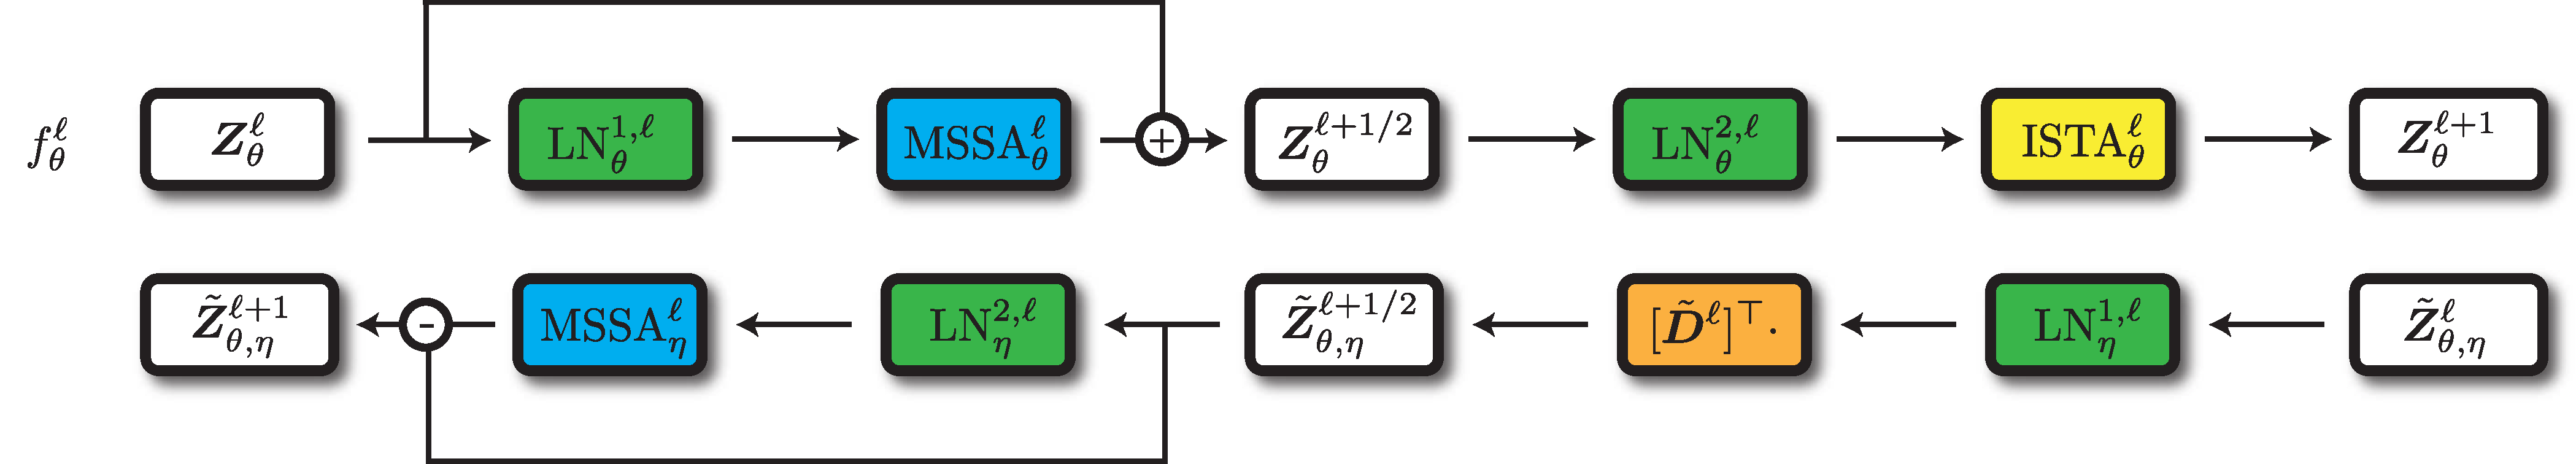
\includegraphics[width=\textwidth]{\toplevelprefix/chapters/chapter7/figs/crate_ae_backbone.pdf}
    \caption{\small\textbf{Un strat al encoder-ului și decoder-ului într-un backbone de autoencoder CRATE.} Straturile encoder-ului și decoder-ului alimentează ambele intrările lor prin auto-atenție de subspațiu multi-cap și un pas de învățare de dicționar sau codare de dicționar. Observați că straturile encoder-ului și decoder-ului sunt proiectate simetric; scopul conceptual al fiecărui strat de decoder este de a inversa un strat de encoder, așa că această simetrie este foarte mult prin design (vezi, de exemplu, \Cref{ch:autoencoding}).}
\end{figure}

Folosim un encoder și decoder CRATE, ilustrat în \Cref{fig:transformer_backbone}, deși, bineînțeles, este posibil să folosim un encoder și decoder transformer obișnuit. Detaliile urmează.

\paragraph{Encoder-ul.} Encoder-ul este același cu encoder-ul CRATE din \Cref{sub:image_classification_architecture}, cu mențiunea că nu există extractor de caracteristici \(f_{\theta}^{\ext}\). Totuși, atât încorporarea \(f_{\theta}^{\emb}\), cât și backbone-ul \(f_{\theta}^{\backbone}\) sunt aceleași.

\paragraph{Backbone-ul decoder-ului.} Backbone-ul decoder-ului este decoder-ul CRATE descris în \Cref{ch:autoencoding}. Pentru completitudine, îl descriem acum. Având o secvență de caracteristici \(\vZ_{\theta}(\vX) \doteq f_{\theta}(\vX) \in (\R^{d})^{*}\), o putem procesa folosind backbone-ul decoder-ului \(g_{\eta}^{\backbone}\) după cum urmează. Funcția \(g_{\eta}^{\backbone}\) este compusă din \(L\) straturi \(g_{\eta}^{\ell}\), adică,
\begin{equation}
    g_{\eta}^{\backbone} = g_{\eta}^{L} \circ \cdots \circ g_{\eta}^{1}.
\end{equation}
Stratul \(g_{\eta}^{\ell}\) are următoarea implementare. Mai întâi, definim \(\tilde{\vZ}_{\theta, \eta}^{1}(\vX) \doteq \vZ_{\theta}(\vX)\). Apoi, obținem
\begin{align}
    \tilde{\vZ}_{\theta, \eta}^{\ell + 1/2}(\vX) 
    &= [\tilde{\vD}^{\ell}]^{\top}\LN_{\eta}^{1, \ell}(\tilde{\vZ}_{\theta, \eta}^{\ell}(\vX)) \\ 
    \tilde{\vZ}_{\theta, \eta}^{\ell + 1}(\vX)
    &= \tilde{\vZ}_{\theta, \eta}^{\ell + 1/2}(\vX) - \MSSA_{\eta}^{\ell}(\LN_{\eta}^{2, \ell}(\tilde{\vZ}_{\theta, \eta}^{\ell + 1/2}))
\end{align}
și \(g_{\eta}^{\ell}\) este definit astfel încât \(g_{\eta}^{\ell}(\tilde{\vZ}_{\theta, \eta}^{\ell}) \doteq \tilde{\vZ}_{\theta, \eta}^{\ell + 1}(\vX)\). Aici, conceptul relevant este că \(g_{\eta}^{\ell}\) ar trebui să învețe o inversă aproximativă a \(f_{\theta}^{L + 1 - \ell}\), ca discretizări ale unui proces de difuzie în timp direct și, respectiv, invers. În special, \(\tilde{\vD}^{\ell}\) ar trebui să aproximeze \(\vD^{L + 1 - \ell}\), și, în mod similar, parametrii \(\MSSA_{\eta}^{\ell}\) ar trebui să fie similari cu parametrii \(\MSSA_{\theta}^{L + 1 - \ell}\). Ieșirea este \(\tilde{\vZ}_{\theta, \eta} \doteq \tilde{\vZ}_{\theta, \eta}^{L + 1}\).

\paragraph{Modulul de des-încorporare.} Pentru a transforma \(\tilde{\vZ}_{\theta, \eta}(\vX)\) înapoi într-o estimare pentru \(\vX\), trebuie să anulăm efectul modulului de încorporare \(f_{\theta}^{\emb}\) folosind modulul de des-încorporare \(g_{\eta}^{\unemb}\). Ca atare, refăcând la forma funcțională a modulului de încorporare din \eqref{eq:definition_of_embedding_module}, adică,
\begin{equation}
    f_{\theta}^{\emb}(\vX) \doteq \mat{\vz_{\cls}^{1}, \vW^{\emb}f^{\patch}(\vX) + \vE^{\pos}}
\end{equation}
implică că operația noastră inversă \(g_{\eta}^{\unemb}\) arată astfel:
\begin{equation}
    g_{\eta}^{\unemb}(\tilde{\vZ}) \doteq g_{\eta}^{\unemb}(\mat{\tilde{\vz}^{1}, \dots, \tilde{\vz}^{n}}) = g^{\unpatch}(\vW^{\unemb}([\tilde{\vz}^{2}, \dots, \tilde{\vz}^{n}] - \tilde{\vE}^{\pos})),
\end{equation}
unde \(g^{\unpatch}\) face operația inversă a operației de derulare și aplatizare pe care o face \(f^{\patch}\).\footnote{Din nou, ``codarea pozițională inversă'' \(\tilde{\vE}^{\pos}\) este învățată pentru o intrare mare și pentru intrări mai mici poate fi interpolată. Este chiar posibil să setăm direct \(\tilde{\vE}^{\pos}\) egal cu codarea pozițională \(\vE^{\pos}\) și să folosim aceleași codări poziționale interpolate pentru fiecare intrare atât în encoder, cât și în decoder.}

Această arhitectură este un autoencoder cu cutie albă \((f_{\theta}, g_{\eta})\) unde (reamintim) \(f_{\theta} = f_{\theta}^{\backbone} \circ f_{\theta}^{\emb}\) și \(g_{\eta} = g_{\eta}^{\unemb} \circ g_{\eta}^{\backbone}\). În special, îl putem folosi pentru a calcula o estimare pentru o vedere mascată \(\hat{\vX}_{\theta, \eta}(\vX_{m}) = (g_{\eta} \circ f_{\eta})(\vX_{m})\) care ar trebui să fie aproximativ egală cu \(\vX\) însăși.

\subsection{Optimizare}\label{sub:image_completion_optimization}

Ca în \Cref{sub:image_classification_optimization}, folosim o configurație simplă de optimizare: eșantionăm imagini și măști, calculăm pierderea pe acele eșantioane și gradienții acestei pierderi și actualizăm parametrii folosind un algoritm de optimizare generic și gradienții menționați mai sus. Pentru fiecare pas de timp \(k\), noi:
\begin{itemize}
    \item Subeșantionăm \(B\) eșantioane diferite \(\{\vX_{b}^{(k)}\}_{b = 1}^{B} \subseteq \cI\).
    \item Pentru fiecare eșantion \(\vX_{b}^{(k)}\), calculăm o decupare redimensionată aleatorie diferită și mască \(v_{b, m}^{(k)}\) și o aplicăm la \(\vX_{b}^{(k)}\) pentru a obține \(\vX_{b, m}^{(k)} \doteq v_{b, m}^{t}(\X_{b}^{(k)})\).
    \item Calculăm autocodarea estimată \(\hat{\vX}_{\theta, \eta}(\vX_{b, r}^{(k)}) \doteq (g_{\eta} \circ f_{\theta})(\vX_{b, r}^{(k)})\).
    \item Formăm pierderea stocastică surogat 
    \begin{equation}
        \hat{\cL}_{\mathrm{MAE}}^{(k)}(\theta, \eta) \doteq \frac{1}{B}\sum_{b = 1}^{B}\norm{\hat{\vX}_{\theta, \eta}(\vX_{b, r}^{(k)}) - \vX_{b}^{(k)}}_{F}^{2}.
    \end{equation}
    \item Calculăm un pas al unui algoritm de optimizare pe \((\theta, \eta)\), dând următoarea iterație:
    \begin{equation}
        (\theta^{(k + 1)}, \eta^{(k + 1)}) \doteq \textsc{OptUpdate}^{(k)}(\theta^{(k)}, \eta^{(k)}; \nabla_{(\theta, \eta)}\hat{\cL}_{\mathrm{MAE}}^{(k)}).
    \end{equation}
\end{itemize}

\subsection{Evaluare} \label{sub:image_completion_optimization_1}

Aceasta este prima rețea de autoencoder pe care o discutăm în acest capitol. Folosim aceeași vedere de decupare centrală \(v_{\cc}\) ca în \Cref{sub:contrastive_learning_evals,sub:image_classification_evals}, redimensionând imaginea finală la un pătrat cu lungimea laturii de \(S_{\cc} = S_{\mask}\) pixeli pentru a potrivi formele imaginilor de intrare văzute în timpul antrenării. 

În plus față de evaluarea pierderii de autocodare cu măști în sine, este de asemenea posibil să evaluăm direct caracteristicile \(\vZ_{\theta}(\vX_{\cc})\) ale vederii \(\vX_{\cc} \doteq v_{\cc}(\vX)\) a datelor \(\vX\). Pentru evaluarea fidelității hărții de atenție, obținerea \(\vZ_{\theta}(\vX_{\cc})\) este suficientă, dar pentru sondarea liniară trebuie să extragem o caracteristică rezumată sau agregată din \(\vZ_{\theta}\). Pentru a face acest lucru, putem folosi o hartă de extracție a caracteristicilor (fără parametri) care returnează caracteristica corespunzătoare token-ului de clasă, adică,
\begin{equation}
    f_{\theta}^{\ext}(\vZ) \doteq f_{\theta}^{\ext}([\vz^{1}, \dots, \vz^{n}]) = \vz^{1},
\end{equation}
ca în (de exemplu) \Cref{sub:image_classification_objective,sub:image_classification_architecture}. Cu aceasta, avem o modalitate de a obține caracteristici agregate \(\vz_{\theta}(\vX_{\cc}) \doteq (f_{\theta}^{\ext} \circ f_{\theta})(\vX_{\cc})\), moment în care putem efectua sondare liniară, evaluări de segmentare și așa mai departe.

\subsection{Experimente}\label{sub:image_completion_experiments}

Deoarece CRATE-MAE se bazează direct pe ViT-MAE, comparăm setările optime pentru ViT-MAE, așa cum sunt date de \citep{he2022masked}, cu aceleași setări aplicate la CRATE-MAE pentru o comparație echitabilă.

\paragraph{Arhitectura modelului.} În timpul antrenării, decuparea mascată \(v_{m}\) redimensionează întreaga imagine astfel încât marginea mai scurtă să fie de dimensiune \(256\) (adică, \(S_{\rsz} = 256\)) înainte de a lua o decupare aleatorie de dimensiune \(224 \times 224\) (adică, \(S_{\mathrm{mask}} = 224\)), și mascând \(p_{\mathrm{mask}} = \frac{3}{4}\) din patch-uri. Luăm dimensiunea patch-ului \(16\) (adică, \(P_{H} = P_{W} = 16\)). Folosim variantele mici și de bază ale arhitecturii ViT-MAE ca încorporare și backbone atât pentru encoder, cât și pentru decoder, schimbând componentele MHSA și MLP pentru MSSA, ISTA și, respectiv, straturi liniare. Folosim același număr de capete și dimensiune a capului în cazul MSSA. Totuși, ViT-MAE original folosește un encoder care folosește aproape toate straturile totale și un decoder care folosește doar câteva straturi; alocăm jumătate din numărul total de straturi (care rămâne același de la ViT-MAE la CRATE-MAE) encoder-ului și decoder-ului nostru, după cum sugerează cadrul conceptual și teoretic din \Cref{ch:autoencoding}. Pentru CRATE-MAE setăm \((\beta, \lambda) = (1, 0.1)\).

\paragraph{Seturi de date și optimizare.} Pentru pre-antrenare, folosim setul de date ImageNet-1K. Folosim optimizatorul AdamW pentru a pre-antrena atât replicația noastră ViT-MAE, cât și CRATE-MAE. Setăm rata de învățare de bază ca \(3 \times 10^{-5}\), decadența ponderii ca \(0.1\) și dimensiunea batch-ului ca \(B = 4096\). Programul nostru de rată de învățare crește rata de învățare liniar până la rata de învățare de bază pe parcursul primelor \(40\) de epoci și scade la \(0\) folosind o programare cosinus pe parcursul următoarelor \(760\) de epoci (antrenând toate modelele pentru \(800\) de epoci fiecare). Pentru pre-antrenare, aplicăm regimul obișnuit de augmentări de date (răsturnări, estompare gaussiană, solarizare etc.) la datele de imagine.

Pentru sondarea liniară, folosim mai multe seturi de date de evaluare, cum ar fi CIFAR10, CIFAR100, Oxford-Flowers și Oxford-IIT-Pets. Pentru sondarea liniară, precalculăm caracteristicile tuturor eșantioanelor din setul de date țintă și aplicăm un rezolvator de regresie liniară rapid, de exemplu, dintr-un pachet standard precum Scikit-Learn.

\paragraph{Rezultatele experimentului.} \Cref{tab:crate_mae_linear_probing} demonstrează că modelele CRATE-MAE obțin, în linii mari, paritate cu populara arhitectură ViT-MAE la număr similar de parametri și, de asemenea, că performanța de învățare a caracteristicilor (măsurată prin performanța la sarcinile de clasificare ulterioare) crește cu scala. Între timp, \Cref{fig:crate_mae_semantic_heads} demonstrează că hărțile de saliență ale encoder-ului (și, prin urmare, caracteristicile fine învățate de encoder) într-adevăr izolează și evidențiază părțile cheie ale imaginii de intrare.


\begin{table}
    \centering 
    \begin{tabular}{@{}lcc|cc@{}}
        \toprule 
        \textbf{Model} & CRATE-MAE-S(mall) & CRATE-MAE-B(ase) & {\color{gray} ViT-MAE-S} & {\color{gray} ViT-MAE-B} \\
        \midrule
        \midrule
        \# parametri & 25.4M & 44.6M & 47.6M & {\color{gray}143.8M} \\
        \midrule
        CIFAR10 & 79.4 & 80.9 & {\color{gray} 79.9} & {\color{gray} 87.9} \\
        CIFAR100 & 56.6 & 60.1 & {\color{gray} 62.3} & {\color{gray} 68.0} \\
        Oxford Flowers-102 & 57.7 & 61.8 & {\color{gray} 66.8} & {\color{gray} 66.4} \\
        Oxford-IIIT-Pets & 40.6 & 46.2 & {\color{gray} 51.8} & {\color{gray} 80.1} \\
        \bottomrule
    \end{tabular}
    \caption{\small\textbf{Acuratețea de clasificare prin sondare liniară a CRATE-MAE și ViT-MAE} pe diverse seturi de date cu diferite dimensiuni ale modelului când backbone-ul este pre-antrenat pentru autocodare cu măști pe ImageNet-1K. Dat fiind același număr de parametri, CRATE-MAE obține performanță aproximativ similară, bucurându-se simultan de un design de arhitectură mai simplu și mai principial.}
    \label{tab:crate_mae_linear_probing}
\end{table}

\begin{figure}
    \centering 
    \includegraphics[width=\textwidth]{\toplevelprefix/chapters/chapter7/figs/crate_mae_semantic_heads.pdf}
    \caption{\small\textbf{Hărți de saliență ale CRATE-MAE.} Fiecare pereche de imagini constă din imaginea originală (stânga) și o hartă de saliență selectată (dreapta) corespunzătoare unui cap de atenție din ultimul strat. După cum este obișnuit pentru modelele CRATE, dar neobișnuit pentru modelele generale de tip transformer, hărțile de saliență corespund obiectelor din imaginea de intrare.}
    \label{fig:crate_mae_semantic_heads}
\end{figure}





\section{Rezumat și note}

Toate lucrările din acest capitol sunt derivate din arhitectura Transformer, care a fost introdusă de \citet{vaswani2017attention}. Arhitectura Transformer este descrisă formal în \Cref{sec:contrastive_learning}. O inovație empirică principală din ultimii ani, stimulată de prevalența și performanța arhitecturii Transformer, este de a formula o problemă de învățare dată ca o problemă secvență-la-secvență și de a aplica arhitectura Transformer. Aceasta a permis arhitecturii Transformer să fie esențial omniprezentă în (aproape) toate aplicațiile de învățare profundă. Ca atare, îmbunătățirile directe ale Transformer-ului pot să se propage pentru a deveni soluții la multe probleme și au un impact considerabil; în mod similar, putem aplica înțelegerea noastră cu cutie albă a arhitecturilor de tip transformer la multe probleme moderne. Materialul acoperit în acest capitol este doar un subset al muncii care a fost deja făcută; alte lucrări includ completarea cu măști pentru date text (adică, BERT) \citep{devlin2019bert,yu2024white}, interpretabilitatea (mecanicistă) a modelelor de limbaj și viziune \citep{bai2024improving} și codarea de corecție a erorilor \citep{zheng2025white}. Există mult mai multe de făcut.

Există, de asemenea, multă mai multă teorie specifică despre practica scalării rețelelor neuronale, care este enorm de viabilă practic, și cel puțin o menționăm aici. Această linie de lucru a fost popularizată de linia de lucru ``Tensor Programs'' \citep{yang2022tensor}. Prescripția de bază este că dorim ca actualizările inițiale ale gradientului într-un transformer să fie de dimensiune constantă și, lucrând cu atenție prin ecuațiile de backpropagare (\Cref{app:optimization}), putem determina scala inițializării și ratele de învățare (alese pe straturi) care sunt necesare pentru a realiza acest lucru. În practică, astfel de prescripții cresc foarte mult stabilitatea și convergența antrenării la scală mare; ele prescriu, de asemenea, o modalitate de a găsi hiperparametrii ``optimi''\footnote{Cuvântul ``optim'' este folosit între ghilimele deoarece lucrările pe acest subiect folosesc doar niște deziderate despre dimensiunea ponderii, dimensiunea caracteristicii și dimensiunea gradientului la inițializare pentru a determina ``optimitatea'', spre deosebire de, să spunem, pierderea de testare la convergență.} pentru antrenarea la scară mare folosind doar antrenare la scară mică. Lucrările ulterioare acestei lucrări încearcă să acomodeze geometria caracteristicilor \citep{bernstein2024oldoptimizernewnorm}, care ar putea fi informată de lucrările din această carte despre învățarea reprezentărilor. Alte lucrări ulterioare încorporează aceste informații despre ponderi în optimizatorul însuși pentru a obține aceste beneficii de scalare automat, obținând optimizatori precum Muon \citep{jordan6muon}, care au fost recent folosite pentru antrenarea modelelor de trilioane de parametri foarte stabil \citep{moonshot2025kimi}. În general, cele două abordări ale teoriei învățării profunde sunt ortogonale sau complementare.


\section{Exerciții și extinderi}

\begin{exercise}
    Citește lucrarea DINO \cite{caron2021emerging}.
\end{exercise}

\begin{exercise}
    DINO v2 \cite{oquab2023dinov2} folosește totul din DINO v1, dar și, în timpul fazei de augmentare a datelor, maschează aleatoriu patch-uri în cadrul fiecărei vederi. Acest tip de augmentare ar trebui să impună ca caracteristicile imaginilor cu informații locale similare să fie similare. Formulează o problemă de optimizare care promovează aceasta în encoder și implementeaz-o.
\end{exercise}


\begin{exercise}
    Acest exercițiu consideră implementarea algoritmilor de optimizare stocastică pentru minimizarea pierderilor care implică așteptări.
    \begin{enumerate}[(a)]
        \item Propune o alternativă la termenul care implică \(R_{\eps}\) din \eqref{eq:simdino_loss_teacherstudent_empirical} pentru aproximarea termenului de regularizare a covarianței din \eqref{eq:simdino_loss_teacherstudent}. Evaluează complexitatea de timp necesară pentru a calcula termenul propus și gradientul său. Include o analiză pentru calcularea acestuia pe un singur nod de calcul vs. mai multe noduri.
        \item Evaluează complexitatea de timp necesară pentru a calcula termenul existent din \eqref{eq:simdino_loss_teacherstudent_empirical} și gradientul său.
    \end{enumerate}
\end{exercise}

\begin{exercise}
    Demonstrează că \eqref{eq:linear_probing} și \eqref{eq:linear_probing_empirical} sunt probleme de optimizare convexe.
\end{exercise}

\begin{exercise}
    \phantom{}
    \begin{enumerate}[(a)]
        \item Implementează modelele CRATE și CRATE-\(\alpha\).
        \item Compară performanța și eficiența lor pe setul de date CIFAR-10.
        \item Compară interpretabilitatea lor în două moduri:
        \begin{itemize}
            \item Sparsitatea \(\norm{\vZ}_{0}\) a reprezentării \(\vZ\)
            \item Hărțile de atenție \(\va_{\theta}^{k, \ell}\)
        \end{itemize}
    \end{enumerate}
\end{exercise}

\end{document}